\newcommand{\cmmnt}[1]{}
\newcommand{\footurl}[2]{\footnote{#1 \href{#2}{\url{#2}}}}
% Bei Abgabe löschen
\documentclass[notables, nomenclature, oneside, 150]{HSMW-Thesis}

\usepackage{enumitem}
\usepackage{setspace}
\usepackage{hyperref}
\hypersetup{
	urlcolor			= black ,
	hidelinks		= true	,
	hyperfootnotes	= false ,
	pdftitle    		= {Entwicklung einer Dokumenten-Scanner-App},
  	pdfsubject  		= {Digitalisierung der Verwaltung an der Hochschule Mittweida},
  	pdfauthor   		= {Hannes Steiner},
  	pdfkeywords 		= {},
  	pdfcreator  		= {pdflatex},
  	pdfproducer 		= {LaTeX with hyperref}
}

\usepackage{subcaption}
\usepackage[section]{placeins}
\usepackage{fancybox, graphicx}
\usepackage[ngerman]{babel}

\Art{Praktikumsbericht}

\Anrede{Herr}
\Vorname{Hannes}
\Nachname{Steiner}

\Thema{Entwicklung einer Dokumenten-Scanner-App}
\Unterthema{Digitalisierung der Verwaltung an der Hochschule Mittweida}

\Studiengang{Softwareentwicklung}
\Seminargruppe{IF17wS-B \\[\bigskipamount] Matrikelnummer:\\ 46540}
\Fakultaet{\MNI}
\Erstpruefer{Prof\@. Dr\@. Marc Ritter}
\Zweitpruefer{Dipl.-Inf. Holger Langner}

\Datum{15.05.2020}

\Tag{15}
\Monat{Mai}
\Jahr{2020}

\Anlagen{}
\Copyright{Dieses Werk ist urheberrechtlich geschützt.}
\Textsatz{}
\Druck{}
\Verlag{}
\ISBN{}


\begin{document}

\begin{Referat}
Im Rahmen eines zwölfwöchigen Forschungspraktikums an der Hochschule Mittweida arbeiteten der Student Tobias Kallauke und der Verfasser des Berichts gemeinsam an einem Projekt mit dem Hintergrund der Digitalisierung der Verwaltung von Lehr- und Forschungseinrichtung. Dabei entwickelten sie ein prototypisches Software-System, mit dessen Hilfe kontrollierte Klausuren eingescannt und digitalisiert werden können.
\end{Referat}

\Hauptteil

%%%%%%%%%%%%%%% - EINLEITUNG - %%%%%%%%%%%%%%%

\chapter{Einleitung}
	Digitalisierung wird gängig als Integration von digitaler Technologie in den Alltag verstanden und soll helfen Zeit einzusparen. Mit diesem Gedanken initiierten die Mitarbeiter Holger Langner und Falk Schmidsberger der Hochschule Mittweida das Projekt Memo Space. Im Zuge dessen sollen kleinere Forschungsergebnisse entstehen, die richtungsweisend für die Digitalisierung der Verwaltung von Lehr- und Forschungseinrichtung sind.

	Im Rahmen eines zwölfwöchigen Forschungspraktikums an der Hochschule Mittweida arbeiteten der Student Tobias Kallauke und der Verfasser des Berichts gemeinsam an einem Forschungsprojekt von Memo Space. Dabei entwickelten sie ein prototypisches Software-System zum Einscannen und Digitalisieren von kontrollierten Klausuren.

%%%%%%%%%%%%%%% - HSMW - %%%%%%%%%%%%%%%

\chapter{Hochschule Mittweida}
	Die Hochschule Mittweida - university of applied science (HSMW) \nomenclature{HSMW}{Hochschule Mittweida - university of applied science} wurde vor über 150 Jahren gegründet. Heute lehrt und forscht sie mit ca. 6000 Studenten in fünf Fakultäten und vier Forschungsschwerpunkten\cite{hochschule_mittweida_hochschule_nodate}. Eines der Schwerpunkte ist die Angewandte Informatik, in dem Memo Space angesiedelt ist.
	
	Nach eigener Einschätzung schreibt jeder Student der HSMW ca. 5 Prüfungen pro Semester. Das bedeutet, dass im Jahr um die 60.000 Klausuren kontrolliert werden. Dazu kommt, dass die Zensuren in das Verwaltungs-Intranet der HSMW eingetragen werden müssen. Dieser Vorgang ist ebenfalls aufwendig, repetitiv und deshalb kognitiv belastend.
	
	Da die Mitarbeiter der Fakultät Angewandte Computer- und Biowissenschaften (Fakultät CB)\nomenclature{Fakultät CB}{Fakultät für angewandte Computer- und Biowissenschaften} Holger Langner und Falk Schmidsberger selbst Klausuren kontrollieren und die Problematik genau kennen, entstand hier eine der ersten Ideen für Memo Space.

%%%%%%%%%%%%%%% - PROBLEMSTELLUNG - %%%%%%%%%%%%%%%

\chapter{Problemstellung}\label{ch:problemstellung}
	An der Kontrolle von Klausuren arbeiten zum Ende eines Semesters Hochschulmitarbeiter über Tage. Diese Aufgabe muss stets mit hoher Konzentration erledigt werden. Auch bei der anschließenden Eingabe der Noten in ein Webformular des Verwaltungs-Intranets der HSMW ist ein kognitiv belastender Navigationsaufwand notwendig. Denn um die Zensuren einzutragen, muss für jeden Studenten zunächst die jeweilige Seminargruppe und anschließend der Studenten-Name herausgesucht werden. Die unübersichtlichen Listen und die hohe Anzahl an Klicks sind für die Hochschulmitarbeiter belastend. Zusätzlich wird die Suche nach der Seminargruppe durch die ähnlich lautenden Bezeichnungen erschwert. Das führt beim Danebenklicken in der Seminargruppen-Liste dazu, dass man sich eventuell in der Navigation verirrt und von vorne beginnen muss.
	
	\section{Digitalisieren der Klausur-Daten}
	Für genau diesen Vorgang wird nach einer effizienteren Lösung gesucht. Die Prüfer sollen effektiv und möglichst zeitsparend diese Aufgabe verrichten, ohne die Überlastung ihrer Aufmerksamkeitsspanne. Zudem ist angedacht, alle relevanten Klausuren-Daten zu digitalisieren und in ein geeignetes Format zu bringen, um sie automatisiert in das Verwaltungs-Intranet überführen zu können. Darüber hinaus empfiehlt es sich, digitale Kopien der Klausuren abzuspeichern, um sie nicht nur analog zu archivieren.
	
	\section{Klausuren-Vorlage}\label{sc:klausuren-vorlage}
	Eine Klausuren-Vorlage bzw. ein Gestaltungsleitfaden für Klausuren der Fakultät Angewandte Computer- und Biowissenschaften bietet außerdem die Möglichkeit der Kontrolle des Prüfers. Durch das vorgegebene Layout der Klausur ist es möglich, Fehler des Prüfers zu erkennen. Die Klausur in \autoref{fig:klausur} ist nach dieser Klausuren-Vorlage angefertigt worden. Auf dem Deckblatt (\ref{fig:seite1}) der Prüfung ist eine Tabelle mit drei Zeilen und jeweils einer Spalte pro Klausur-Aufgabe. In der ersten Zeile befinden sich die Nummern der Aufgaben, in der zweiten die zu erreichenden Punkte der Aufgabe. In der dritten Zeile trägt der Prüfer die erbrachten Punkte des Studenten ein. Unter der Tabelle befindet sich ein Feld für die erreichte Gesamtpunktzahl sowie ein weiteres für die aus den Punkten resultierende Note. Es soll nun überprüft werden, ob die Summe der erreichten Punkte mit der Gesamtpunktzahl übereinstimmt. Zudem wird auch die Note errechnet und mit dem Ergebnis des Prüfers verglichen werden. Ein weiteres Merkmal der Klausuren-Vorlage ist ein Feld, für die vom Studenten erreichten Punkte über jeder Aufgabenstellung auf den nachfolgenden Seiten. Zu sehen sind solche Felder in \autoref{fig:seite2} am rechten Seitenrand. Die dortige Angabe sollte mit der Angabe in der Tabelle auf dem Deckblatt (\ref{fig:seite1}) übereinstimmen und bietet somit noch eine weitere Möglichkeit der Kontrolle.
	
	\begin{figure}[h!]
    	\centering
   		\begin{subfigure}[t]{0.48\textwidth}
        	\frame{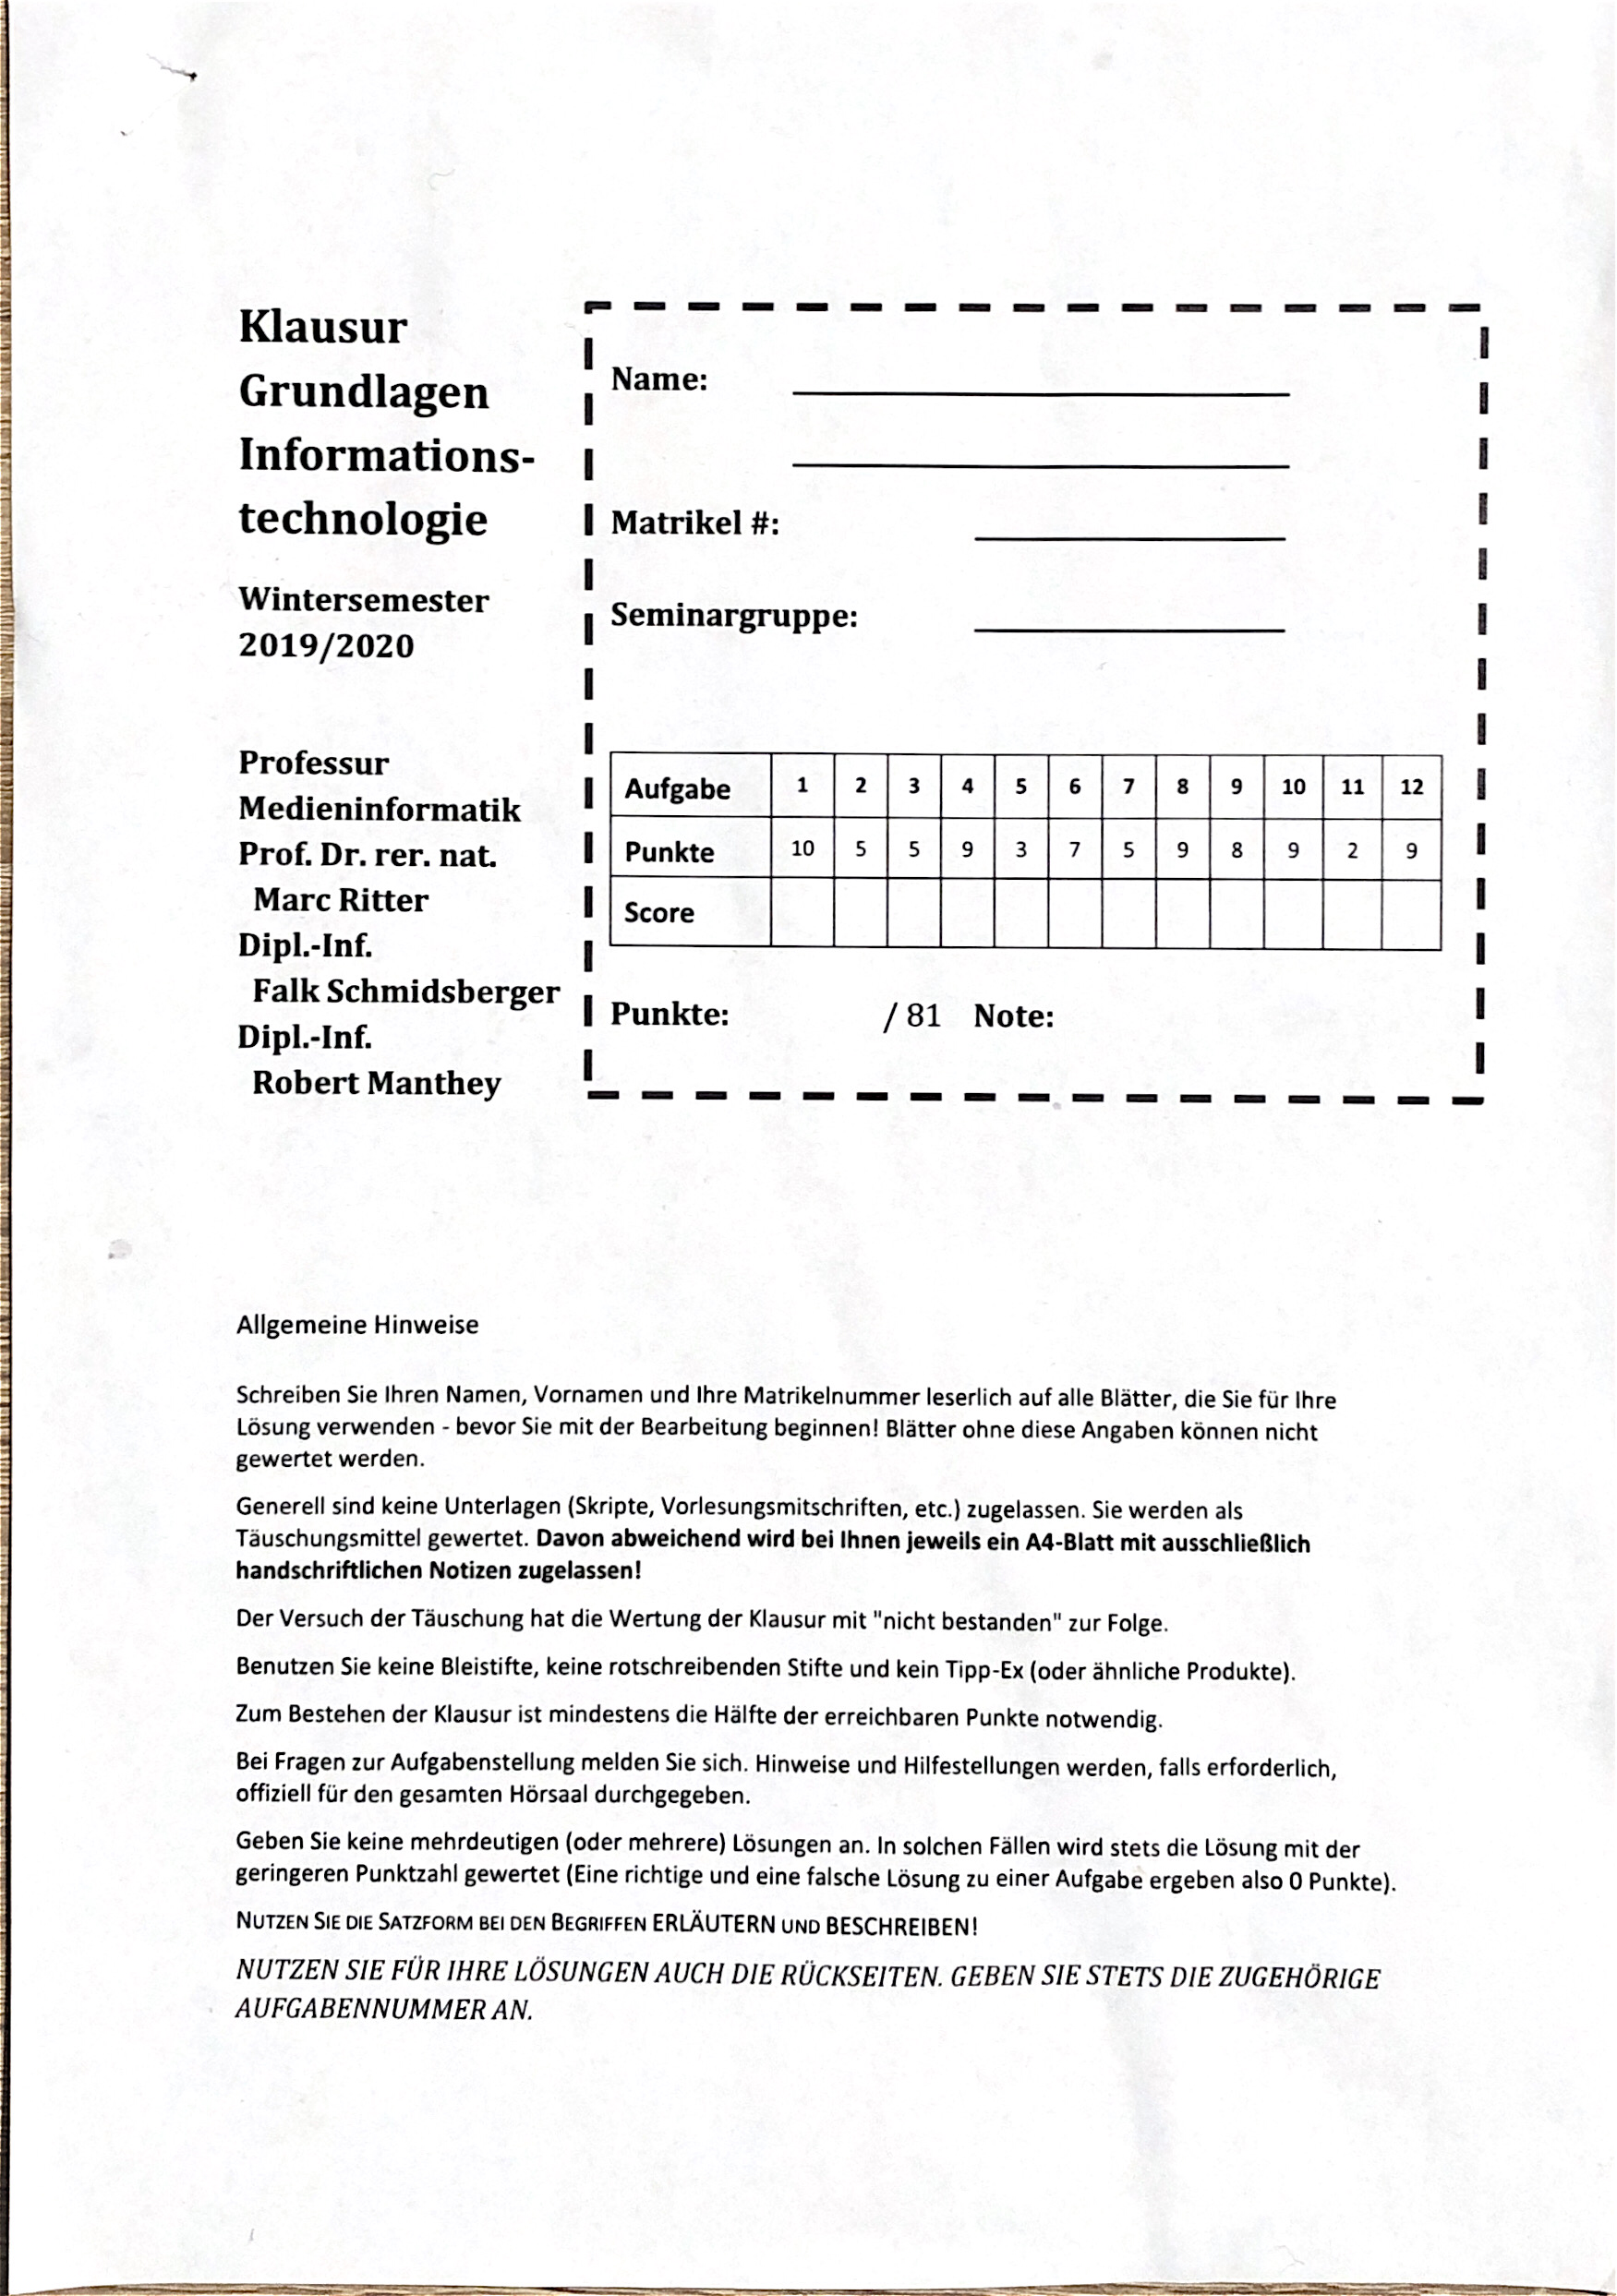
\includegraphics[width=0.96\textwidth]{img/seite1}}
       		\caption{Deckblatt der Klausur}
        	\label{fig:seite1}
    	\end{subfigure}
    	\begin{subfigure}[t]{0.48\textwidth}
        	\frame{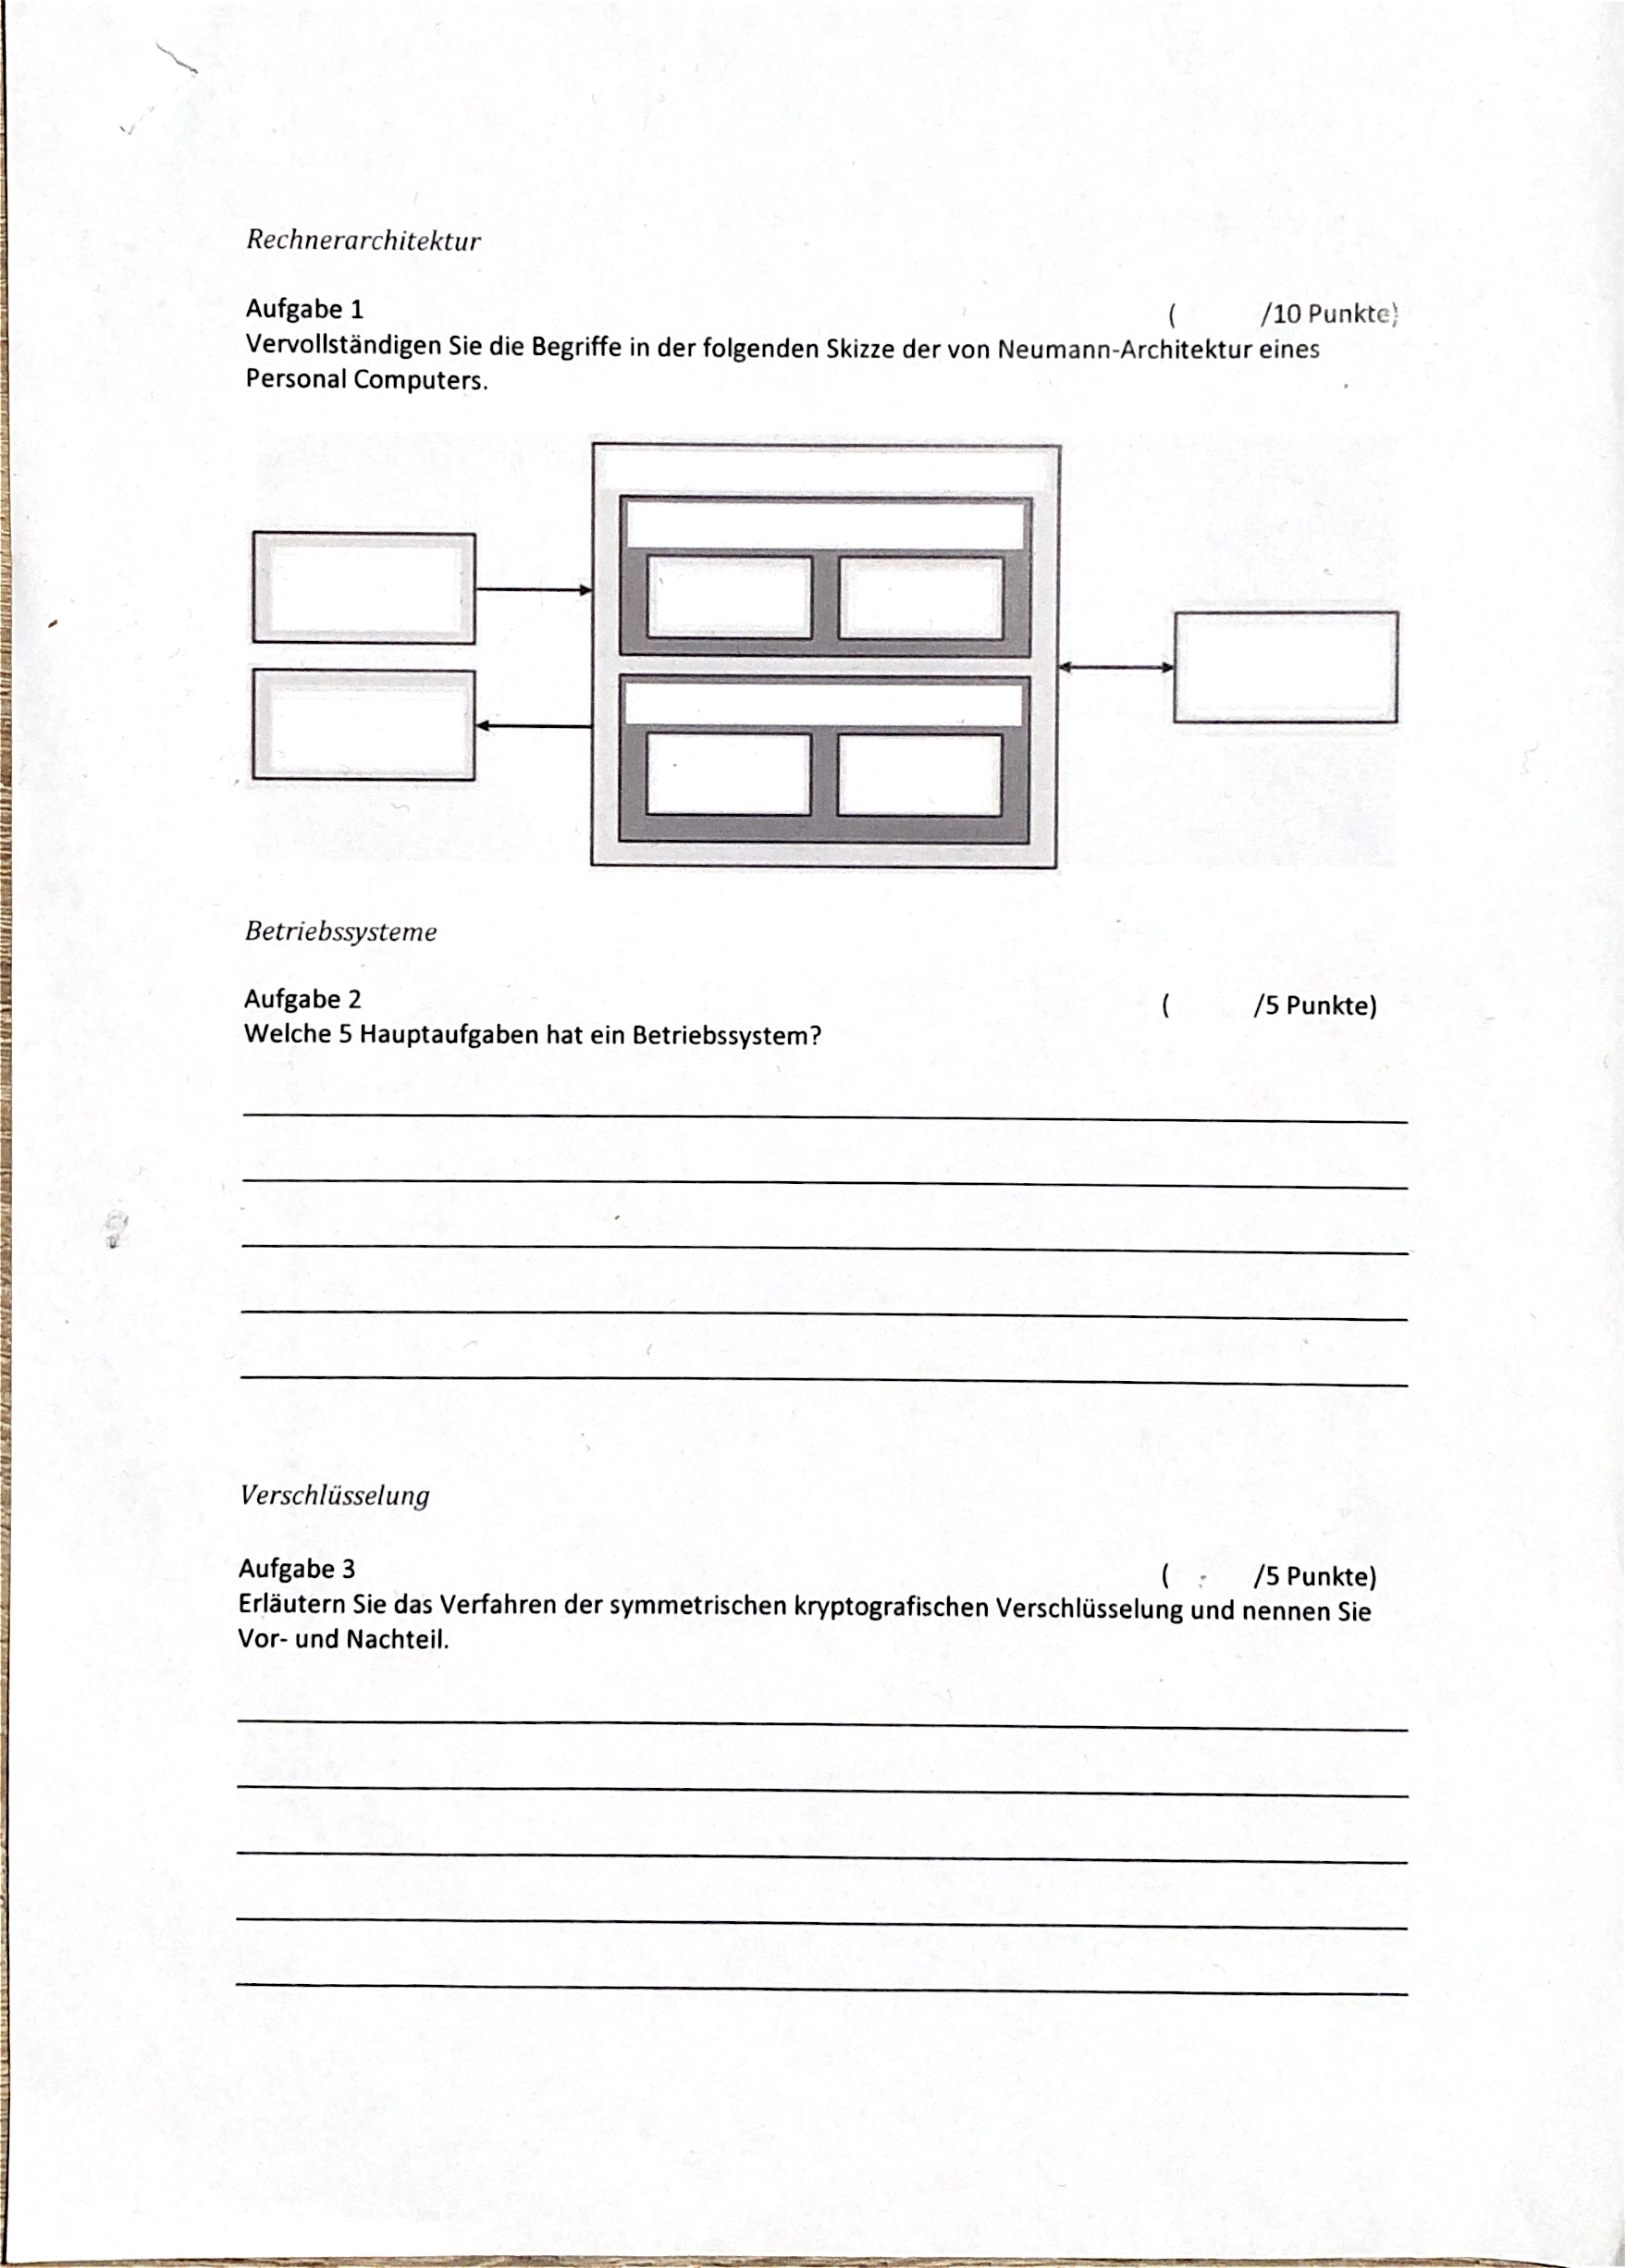
\includegraphics[width=0.96\textwidth]{img/seite2}}
        	\caption{Erste Seite der Klausur mit drei Aufgaben}
        	\label{fig:seite2}
    	\end{subfigure}
    	\caption{Umsetzung der Klausuren-Vorlage der Fakultät CB}
    	\caption*{\textit{Die Bilder sind beim Erstellen einer Scan-Vorlage mit der App entstanden.}}
    	\label{fig:klausur}
	\end{figure}
	
	\section{Klausuren-Vorlage verbessern}
	Nachdem ein erster Prototyp zum Digitalisieren der Klausur-Daten entwickelt wurde, sollen außerdem Klausuren-Vorlagen entstehen, die für die Digitalisierung optimiert sind. Dabei sollten Probleme, die beim Einscannen der aktuellen Vorlage erkannt wurden, behoben werden. 
	
%	\section{Weitere Anmerkungen}
%	Ferner soll bei der Problemlösung von der Anschaffung neuer Technologien und Geräte abgesehen werden. Grund dafür ist neben den Anschaffungskosten, die Idee, dass das Ergebnis des Forschungsprojekts in weiteren Lehr- und Forschungseinrichtungen Anwendung findet. Außerdem hat so gut wie jeder Mitarbeiter an einer Lehr- und Forschungseinrichtung ein eigenes oder Zugang zu einem Smartphone oder Tablet, welche durch die eingebaute Technik in der Lage sind, diese Aufgabe zu übernehmen. 

%%%%%%%%%%%%%%% - ANFORDERUNGEN - %%%%%%%%%%%%%%%

\chapter{Anforderungen}\label{ch:anforderungen}
	In diesem Kapitel werden die Anforderungen an das Software-System dargestellt.

	Es soll eine App für das Betriebssystem iOS entstehen, mit der Klausuren digitalisiert werden können. Dabei müssen die, für die Notenfreigabe relevanten Daten der Klausur, in ein tabellarisches Format gebracht werden. Ferner muss die iOS-Anwendung Bilder von ausgefüllten Prüfungen aufnehmen können und den Inhalt mithilfe von Texterkennung digitalisieren. 
	
	Auch bei unterschiedlicher Seitengestaltung der Klausuren, soll die App in der Lage sein, alle relevanten Informationen, wie z. B. Name, Matrikelnummer und Note richtig zu lokalisieren und anschließend zu digitalisieren. Dafür muss der Benutzer digitale Vorlagen, sogenannte Scan-Vorlagen erstellen. Mit deren Hilfe können, die Informationen sofort gefunden und schneller digitalisiert werden, ohne die gesamte Klausuren-Seite zu verarbeiten. 

	Zusätzlich soll es dem Benutzer möglich sein, Kontrollmechanismen festzulegen. Wie im \autoref{sc:klausuren-vorlage} beschrieben, kann überprüft werden, ob die Punkte auf dem Deckblatt mit den Punkten auf den nachfolgenden Seiten übereinstimmen. Des Weiteren wird kontrolliert, ob die Gesamtpunktzahl korrekt summiert sowie die daraus resultierende Note richtig errechnet wurde. Ein Kontrollmechanismus soll so gestaltet sein, dass diese Überprüfungsmöglichkeiten vom Benutzer bestimmt werden können. Bei Nichtübereinstimmung der genannten Kriterien erhält der Benutzer eine entsprechende Fehlermeldung. % Beispielsweise hat der Prüfer auf dem Deckblatt fünf Punkte eingetragen, bei der Aufgabenstellung auf den nachfolgenden Seiten jedoch eine sechs. Die App muss dann eine Fehlermeldung ausgeben, dass die Punktezahlen bei der Aufgabe nicht übereinstimmen und nochmals kontrolliert werden müssen. 
 
	Um alle relevanten Daten zu erfassen werden die kontrollierten Klausuren zunächst fotografiert. Bei der anschließenden Digitalisierung aller Schriftzeichen durch die App findet optische Zeichen- bzw. Texterkennung Anwendung. Für die Texterkennung auf externen Servern müssen die entsprechenden Server-Schnittstellen zur Kommunikation implementiert werden. 
	 
	Die durch die Texterkennung digitalisierten Daten, die Klausuren-Fotos und die digitalen Scan-Vorlagen sollen außerhalb der App auf einem Server gespeichert werden. Somit können alle Benutzer der App die bereits erstellten Scan-Vorlagen verwenden. Wie bereits erwähnt, werden die digitalisierten Daten zudem in ein geeignetes Format gebracht, um sie, wie angedacht, automatisiert in das Verwaltungs-Intranet zu überführen.
	
	Damit Synchronität der Daten zwischen allen Apps und dem Server gewährleistet werden kann, sind auf beiden Seiten Schnittstellen notwendig. Diese sollten den standardmäßigen CRUD\nomenclature{CRUD}{Das Akronym CRUD steht für Create/Erstellen, Read/Lesen, Update/Aktualisieren und Delete/Löschen und umfasst die vier grundlegenden Operationen persistenter Speicher}-Operationen entsprechen. Für genauere Details zu den Sicherheitsmechanismen und den CRUD-Operationen zum Server siehe im Praktikumsbericht von Tobias Kallauke. 

%%%%%%%%%%%%%%% - GRUND IDEE ZUM LÖSEN DES PROBLEMS - %%%%%%%%%%%%%%%

\chapter{Konzept der Dokumenten-Scanner-App}\label{ch:konzept}
	Dieses Kapitel beschreibt, wie das Softwaresystem die Anforderungen umsetzt.
	
	\section{Scan-Vorlage erstellen und speichern}
	
		Im folgenden Abschnitt wird zuerst verkürzt und anschließend detailliert geschildert, wie eine Scan-Vorlage zu erstellen ist.
    
		Um wirklich nur relevante Daten zu digitalisieren, benötigt es die sogenannten Scan-Vorlagen, die in der App durch den Benutzer angelegt werden können. Eine Scan-Vorlage beinhaltet mehrere Schablonen. Solch eine Schablone wird beispielsweise auf das Deckblatt gelegt, sodass nur noch die relevanten Informationen, die digitalisiert werden sollen, zu sehen sind. Alles andere, was nicht von Interesse ist, wird von der Schablone überdeckt. In der \autoref{fig:schablone1} ist dieses Konzept schemenhaft zu sehen. Der Benutzer kann in zwei grobe Schritte, um eine digitale Schablone anzufertigen. Zuerst muss ein Foto von der Seite aufgenommen werden. Anschließend werden die Regionen auf diesem Foto manuell markiert, die digitalisiert werden sollen. Eine Scan-Vorlage ist somit eine Sammlung aller digitalen Schablonen zu einer Klausur, denn jede Seite benötigt eine eigene individuelle Schablone.
				
		\begin{figure}[h!]
    		\centering
    		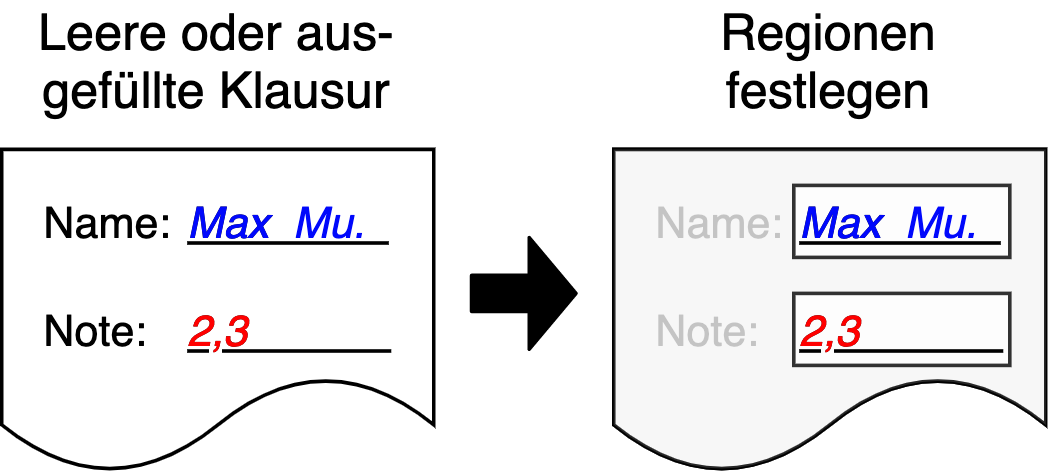
\includegraphics[width=0.48\textwidth]{img/schablone1}
    		\caption{Schematisches Schaubild zum Verständnis des Schablonen-Konzepts}
    		\label{fig:schablone1}
    	\end{figure}
		
		Nachfolgend wird detailliert das Erstellen einer Scan-Vorlage beschrieben. Der Vorgang ist in \autoref{fig:kompakterstellen} als kompaktes Flussdiagramm und in \autoref{fig:schema1} schematisch dargestellt.
		
		 \begin{figure}[th]
    		\centering
    		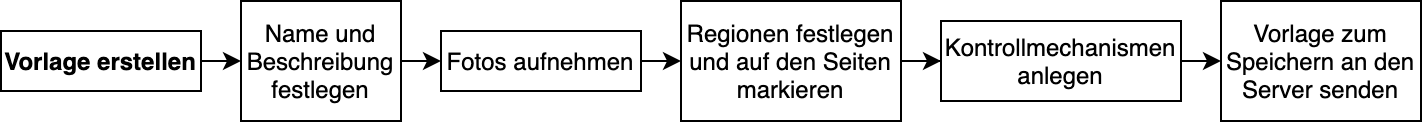
\includegraphics[width=\textwidth]{img/erstellen_flow_small}
    		\caption{Kompaktes Flussdiagramm zum Erstellen einer Scan-Vorlage}
    		\label{fig:kompakterstellen}
    	\end{figure}
	
		\begin{enumerate}
			\item Zu Beginn wird der Scan-Vorlage ein Name und eine Beschreibung gegeben. Anschließend muss jede Seite der Klausur fotografiert werden. Dabei wird in jedem Bild das Dokument erkannt, vom Hintergrund getrennt bzw. ausgeschnitten und perfekt ausgerichtet. Zudem wird der Kontrast erhöht, sodass die Schrift leichter lesbar ist. Die \autoref{fig:klausur} resultiert aus dem Prozess (siehe auch \autoref{fig:v3}). 
		
			\item Anschließend markiert der Benutzer diejenigen Regionen auf jeder Seite, die zu digitalisieren und/oder zu kontrollieren sind. In dem Schema \ref{fig:schema1} sind die Regionen blau hinterlegt (siehe auch \autoref{fig:v9}). Zusätzlich muss jeder Region eine Bezeichnung und einer der folgenden Datentypen zugeordnet werden: Unbekannt, Vorname, Nachname, Matrikelnummer, Seminargruppe, Punkte und Note (siehe auch \autoref{fig:v8} und \ref{fig:v9}).\\
			Die Angabe des Datentyps ist wichtig, da dadurch die Texterkennung optimiert wird und die Ergebnisse der Texterkennung in das geeignete Format gebracht werden können. \label{it:zwei}
			% Die Angabe des Datentyps ist wichtig, da dadurch eindeutig wird, ob es sich um die Note oder den Vornamen des Studenten handelt. Diese Eindeutigkeit wird nicht nur für die automatische Erstellung der Tabelle benötigt, sondern auch für die Optimierung der Texterkennung. \label{it:zwei}
			
			\item Zuletzt wird die Vorlage zum Speichern an einen Server gesendet, wodurch alle Benutzer der App die bereits erstellten Scan-Vorlagen verwenden können.
		\end{enumerate}
		
		\begin{figure}[h!]
    		\centering
    		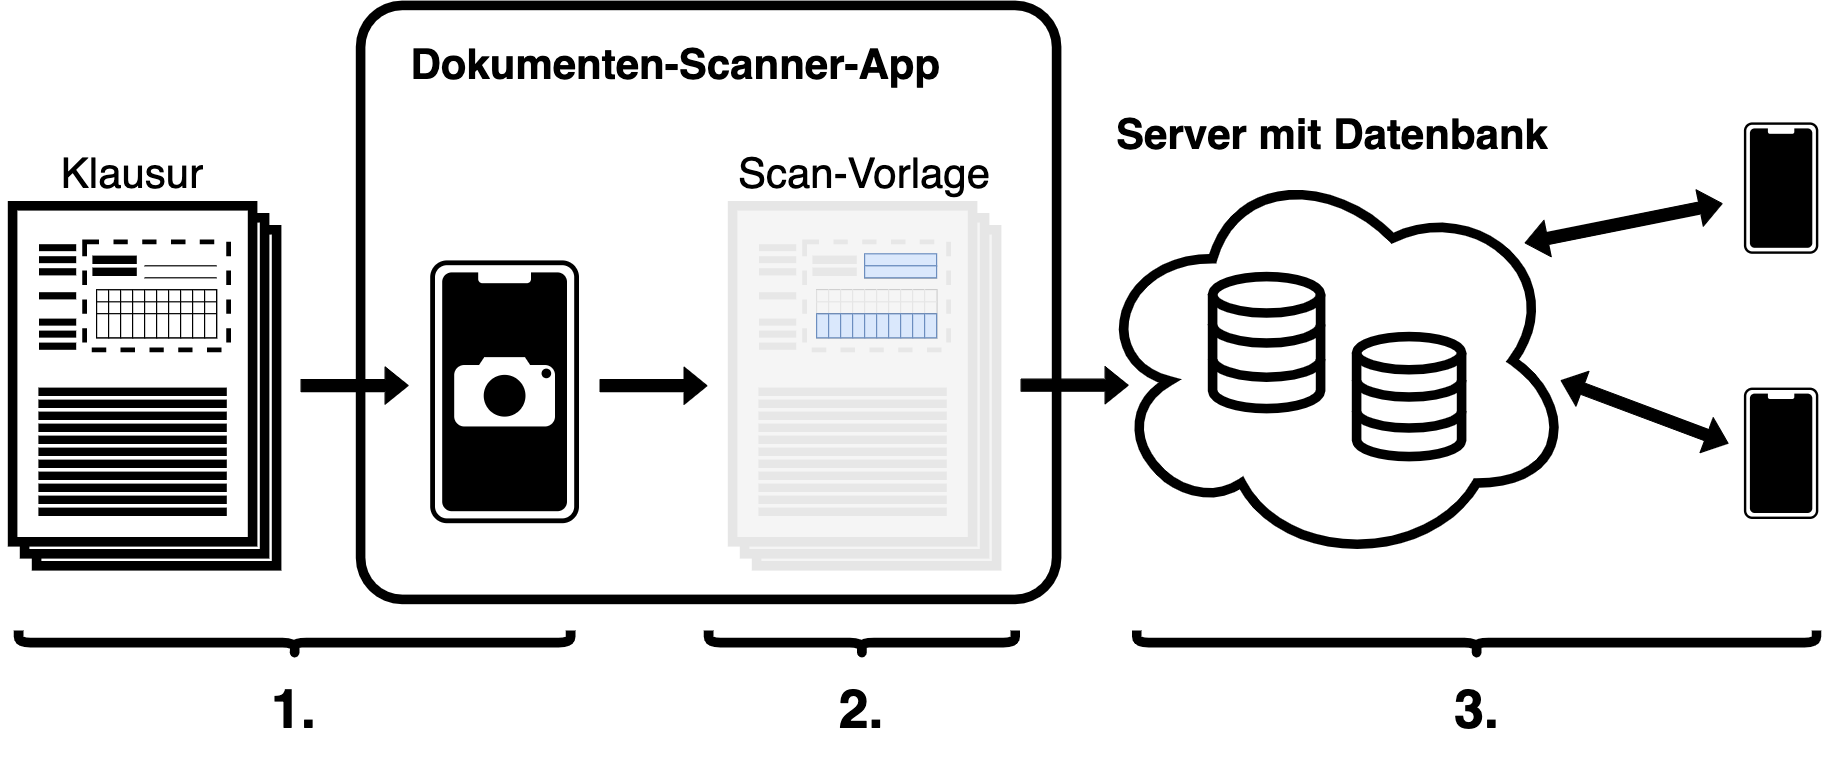
\includegraphics[width=\textwidth]{img/schema1}
    		\caption{Schematische Darstellung des Vorgangs Scan-Vorlage erstellen und auf dem Server speichern}
    		\label{fig:schema1}
    	\end{figure}
		
		%Kontrolle
 		Zusätzlich können in der Phase der Erstellung einer Scan-Vorlage die in \autoref{ch:anforderungen} beschriebenen Kontrollmechanismen festgelegt werden. Dies geschieht nach \autoref{it:zwei}, also nachdem alle Regionen angelegt wurden. Diese Kontrollmechanismen beruhen auf zwei simplen Konzepten. 

 		Das erste Konzept ist der Vergleich. Zur Erinnerung: Es sollen die eingetragenen Punkte auf dem Deckblatt mit den Punkten neben der Aufgabenstellung auf den nachfolgenden Seiten auf Gleichheit überprüft werden. Das zweite Konzept baut auf dem ersten auf. Statt zwei Regionen bzw. Komponenten zu vergleichen, wird eine oder werden beide Komponenten zuvor berechnet. Beispielsweise muss die Summe der Punkte pro Aufgabe mit der Gesamtpunktzahl übereinstimmen. Das bedeutet, es wird erst die Summe berechnet und anschließend mit der vom Prüfer eingetragenen Punktzahl verglichen. Oder aus der Gesamtpunktzahl wird die Note ermittelt und mit der vom Prüfer eingetragen Note verglichen. 
 	
 		Beim Festlegen der Kontrollmechanismen wird wie folgt vorgegangen:
 		\vspace{-5mm}
 		\begin{enumerate}
 			\item Der Benutzer wählt einen Kontrollmechanismus aus. Zur Auswahl stehen:
 				\vspace{-5mm}
 				\begin{itemize}
 					\item der Vergleich zweier Regionen,
 					\item die Gesamtpunktzahl berechnen und mit der eingetragenen Gesamtpunktzahl vergleichen,
 					\item oder die Note aus der Gesamtpunktzahl berechnen und mit der eingetragenen Zensur vergleichen.
 				\end{itemize}
 			\item Aus den zuvor angelegten Regionen müssen nun die passenden Regionen ausgewählt werden. Abhängig von dem gewählten Kontrollmechanismus wird dem Benutzer Auskunft darüber gegeben, welche und wie viele Regionen auszuwählen sind.
 			\item Der Kontrollmechanismus kann gespeichert werden, sobald in jeder zu vergleichenden Komponente die Mindestanzahl an auszuwählenden Regionen erreicht wurde. Diese werden in der Scan-Vorlage hinterlegt und mit an den Server zum Speichern gesendet. So besitzen alle Benutzer dieselben Kontrollmechanismen  zu den jeweiligen Scan-Vorlagen.
 		\end{enumerate}

 	\section{Scan-Vorlage verwenden}
 		Im folgenden Abschnitt wird zuerst verkürzt und anschließend detailliert die Verwendung und Funktionsweise einer erstellten Scan-Vorlage beschrieben. 
 	
 		\begin{figure}[h!]
    		\centering
    		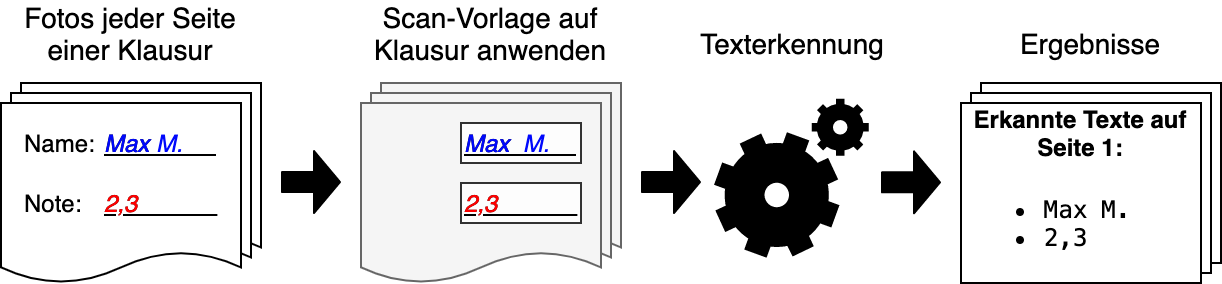
\includegraphics[width=0.95\textwidth]{img/schablone2}
    		\caption{Schematischer Ablauf beim Verwenden einer Scan-Vorlage}
    		\label{fig:schablone2}
    	\end{figure}
 
		Nach dem Erstellen einer Scan-Vorlage kann diese auf bewerteten Klausuren angewandt werden. In \autoref{fig:schablone2} wird der Ablauf schematisch dargestellt. Zuerst werden die Seiten einer Klausur fotografiert. Anschließend stellen die digitalen Schablonen die relevanten Informationen jeder Seite für den nächsten Schritt zur Verfügung. Optical character recognition (OCR)\nomenclature{OCR}{optical character recognition, deutsch: optische Zeichenerkennung und im deutschen Synonym für Texterkennung}, auf deutsch optische Zeichenerkennung, wird dazu benutzt, die Daten aus den übrig gebliebenen Regionen zu digitalisieren.
    	
    	Nachfolgend wird detailliert das Verwenden einer Scan-Vorlage beschrieben. Der Vorgang ist in \autoref{fig:kompaktverwenden} als kompaktes Flussdiagramm und in \autoref{fig:schema2} schematisch dargestellt.

    	
    	\begin{figure}[h!]
    		\centering
    		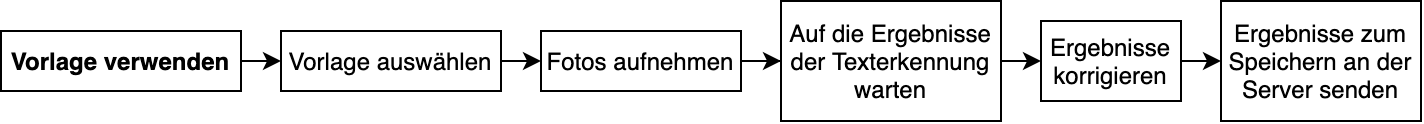
\includegraphics[width=\textwidth]{img/verwenden_flow_small}
    		\caption{Kompaktes Flussdiagramm zum Verwenden einer Scan-Vorlage}
    		\label{fig:kompaktverwenden}
    	\end{figure}
	
		\begin{enumerate}
			\item Die Seiten der Klausur müssen dazu in derselben Reihenfolge, wie in der Scan-Vorlage fotografiert werden. Anschließend werden die Regionen der Scan-Vorlage auf das jeweilige Bild angewendet. Bei dem Prozess entstehen Bildausschnitte, in denen die relevanten Informationen enthalten sind.
			\item Die entstandenen Bildausschnitte werden seitenweise in die Texterkennung überführt.
			\item \label{it:ocr} Die Inhalte der Ausschnitte werden mithilfe von OCR digitalisiert. Der Datentyp der zugehörigen Region aus der Scan-Vorlage nimmt nun Einfluss auf das Ergebnis. Durch ihn wird während der Worterkennungsphase in der Texterkennung eine Liste an vordefinierten möglichen Ergebnissen eingespeist. Diese Liste hat Vorrang vor dem sogenannten Standard-Wörterbuch und verbessert dadurch die Ergebnisse. Ein Beispiel für solch eine Liste können alle möglichen Noten sein. Es ist auch vorstellbar, dass alle Seminargruppen oder Namen von Personen, die an der Klausur teilgenommen haben, dort verwendet werden.
			\item Die Ergebnisse werden im Anschluss an den Server gesendet. Zuvor kann der Benutzer jedoch die Ergebnisse anpassen bzw. korrigieren, falls es bei der Texterkennung zu Fehlern kam. Auch die Kontrollmechanismen finden vor dem Hochladen zum Server Anwendung und geben dem Nutzer durch Fehlermeldungen Hinweise. \label{it:senden}
		\end{enumerate}

		\begin{figure}[h!]
    		\centering
    		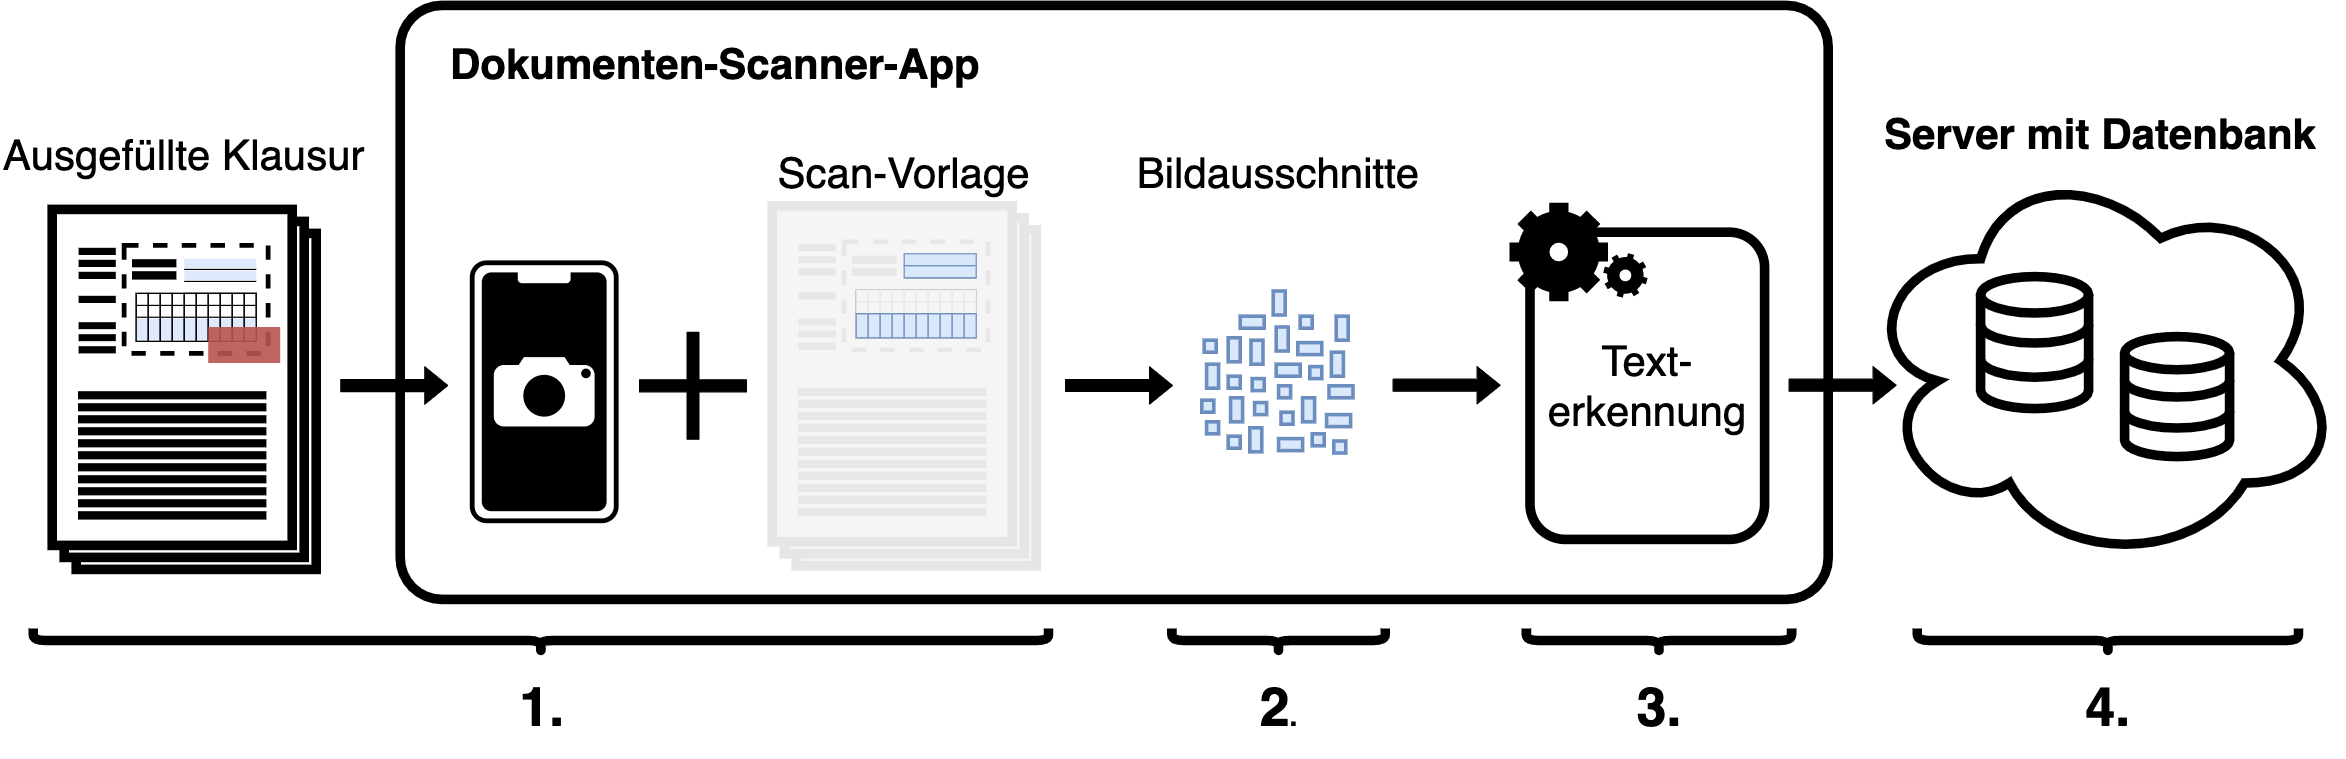
\includegraphics[width=\textwidth]{img/schema2}
    		\caption{Schematische Darstellung des Vorgangs beim Verwenden einer Scan-Vorlage}
    		\label{fig:schema2}
    	\end{figure}
		
	\section{Erweiterung des Konzepts}\label{sc:erweiterungkonzept}
		Weiter ist eine zusätzliche Korrektur angedacht. Angenommen ein Student verschreibt sich bei seiner Seminargruppe und vergisst ein Zeichen. Die Texterkennung erkennt zwar jedes Zeichen, jedoch nicht die korrekte Bezeichnung der Seminargruppe. Deshalb sollte nach der Texterkennung die falsche Bezeichnung durch diejenige Seminargruppe ersetzt werden, die die größte Übereinstimmung mit der erkannten Bezeichnung hat. Bei diesem Vorgehen ist zu beachten, dass nur die Seminargruppen verwendet werden sollten, die tatsächlich die Klausur geschrieben haben. Ähnliches ist auch für die Namen oder Matrikelnummern der Studenten möglich.
		
		Allerdings entstehen auch durch das OCR Fehler. Aus diesem Grund wird neben jedem Ergebnis die sogenannte confidence angezeigt. Diese sagt aus, wie sicher die Texterkennung des Ergebnisses ist. Jedoch kann es auch hier falsche Positiv-Ergebnisse geben. Deshalb ist auch die confidence kein perfekter Indikator für die Richtigkeit des Ergebnisses. Deswegen gibt es, wie in \autoref{it:senden} beschrieben, die Möglichkeit, die Ergebnisse noch einmal zu überprüfen und zu korrigieren, bevor sie an den Server zum Abspeichern gesendet werden. Auch die Kontrollmechanismen reagieren auf die Änderungen der Ergebnisse, sodass Fehlermeldungen behoben werden können.

%%%%%%%%%%%%%%% - PROTOTYP - %%%%%%%%%%%%%%%

\chapter{Entwicklung des ersten Prototyps}\label{ch:prototyp}
	Dieses Kapitel beschreibt einzelne Phasen der Entwicklung der iOS-App in einer ähnlichen Reihenfolge, wie im Wasserfall-Model zur Verwaltung der Entwicklung großer Softwaresysteme nach Winston W. Royce \cite{royce_managing_1970} (siehe \autoref{fig:waterfall}).
    	
	\section{Anforderungsplanung}\label{sc:anforderungsplanung}
	Vor Beginn des Praktikums wurde diskutiert und kalkuliert, welches Thema aus dem Projekt Memo Space für ein zwölfwöchiges Praktikum geeignet ist. Dabei entstand eine Art Durchführbarkeits- / Machbarkeitsstudie, welche zur Entscheidung führte, das Dokumenten-Scanner-Softwaresystem zu entwickeln. Tobias Kallauke soll aufgrund seiner Kenntnisse und Erfahrungen ein Backend mit entsprechenden Schnittstellen und eine Android-App erstellen, während der Verfasser eine iOS-App programmiert. Die iOS-Anwendung soll den Anforderungen, die im gleichnamigen \autoref{ch:anforderungen} zu finden sind, erfüllen. Weitere Details über den Server, dessen Architektur und die Android-App sind im Praktikumsbericht von Tobias Kallauke beschrieben.


\section{Analyse und Definition}\label{sc:analyse}
		Die Aufgaben bzw. Ziele dieser Phase sind: 
		\vspace{-5mm}
		\begin{enumerate}
			\item die Auseinandersetzung mit der Problemstellung und den Anforderungen,
			\item die Durchführung einer Problemanalyse,
			\item die Entwicklung von Ideen und eines genauen Konzepts der iOS-App sowie 
			\item das Entwickeln eines ersten minimalen Prototyps als Machbarkeitsnachweis.
		\end{enumerate}

		Bei der Entstehung des Konzepts, welches im \autoref{ch:konzept} zu finden ist, spielen die Dokumentationen der Frameworks Vision\footurl{Dokumentation von Vision -}{https://developer.apple.com/documentation/vision}, VisionKit\footurl{Dokumentation von VisionKit -}{https://developer.apple.com/documentation/visionkit} und PhotoKit\footurl{Dokumentation von PhotoKit -}{https://developer.apple.com/documentation/photokit} von Apple eine entscheidende Rolle. Aus ihnen geht hervor, welche Funktionen der App noch zu entwickeln und welche in Frameworks schon vorhanden sind. Z. B. ist das Erkennen und das Geradeziehen von Dokumenten in Echtzeit sowie die Texterkennung auf Bildern in Vision und VisionKit enthalten. Bei der Entwicklung des ersten minimalen Prototyps half eine Beispiel-App von Apple \cite{apple_detecting_2019}, die das Erkennen von Objekten in Standbildern mithilfe der genannten Frameworks umsetzt.
		
		Durch die Auseinandersetzung mit den Bibliotheken konnte festgestellt werden, dass die zu entwickelnde App nur Geräte ab der Betriebssystem-Version iOS 13.0 unterstützen wird. Grund dafür sind die Apple Frameworks SwiftUI und VisionKit. \\
		SwiftUI bietet die Möglichkeit, Benutzeroberflächen für alle Apple-Plattformen in der Programmiersprache Swift zu erstellen. Die deklarative Swift-Syntax ist einfach zu lesen und schnell zu schreiben, sodass es möglich ist, die App in wenigen Wochen für iPhone und iPad zu entwickeln. Als Alternative gibt es UIKit\footurl{Dokumentation von UIKit -}{https://developer.apple.com/documentation/uikit}, welches unter allen iOS Versionen funktioniert. Dieses Framework ist allerdings nicht deklarativ, sodass Views sowohl im Code, als auch in Interface-Dateien getrennt voneinander erstellt und konfiguriert werden müssen \cite{sillmann_einstieg_2019}. Dadurch dauert die Entwicklung einer App im Gegensatz zu SwiftUI deutlich länger, wie man auch in dem Video\footurl{SwiftUI vs UIKit – Comparison of building the same app in each framework -}{https://www.youtube.com/watch?v=qk2y-TiLDZo} von Paul Hudson, einem in der Swift-Community sehr bekannten Programmierer und Autor, sieht. Sehr ähnliche Erfahrung hat der Verfasser vor dem Praktikum in seiner Freizeit mit den beiden Frameworks gesammelt. \\
		VisionKit dagegen ist das Framework zum Scannen der Dokumente. Auch hierfür existiert eine Alternative, welche auch auf älteren iOS Versionen funktioniert. Allerdings unterstützt das Framework WeScan\footurl{WeScan GitHub Repository -}{https://github.com/WeTransfer/WeScan} noch kein stapelweises Scannen. Das bedeutet, dass man immer nur ein Foto machen kann, welches erst abgespeichert werden muss, bevor man das nächste aufnehmen kann. Das ist für den Benutzer umständlich und zeitintensiv. Zu Informationen anderer verwendeter Frameworks siehe im \autoref{ch:prototyp} \autoref{sc:implementierung} und \autoref{sc:implementierung}.

		Zur Projektplanung und zum Projektmanagement wurde das Scrum-Konzept\footurl{Der Scrum Guide™ -}{https://www.scrumguides.org/scrum-guide.html}, welches sich für agile Softwareentwicklung anbietet, verwendet. Als Versionsverwaltung der App-Software wurde Git\footurl{Git Internetseite -}{https://git-scm.com/} in Kombination mit GitHub Issues\footurl{Mastering Issues -}{https://guides.github.com/features/issues/} und GitHub Project Boards als Planungstools benutzt. Dadurch konnte der Verfasser jedem sogenannten Sprint selbständig Aufgaben zuordnen und den Fortschritt nachvollziehen. Informationen über den Server und der Android-App zu diesem Thema sind im Praktikumsbericht von Tobias Kallauke zu finden.	

	\section{Grundlagen}
		In den folgenden zwei Absätzen werden wichtige Konzepte erläutert und Grundwissen vermittelt, die im nachfolgendem \autoref{sc:entwurfunddesign} nochmals thematisiert werden.
		
		\vspace{-5mm}
		\paragraph*{Model-View-ViewModel}
			Model-View-ViewModel (MVVM) \nomenclature{MVVM}{Model-View-ViewModel} ist ein Software-Architekturmuster. Unter einem Software-Architekturmuster oder auch Entwurfsmuster ist eine bewährte Lösungsvorlage für wiederkehrende Entwurfsprobleme zu verstehen. MVVM erleichtert die Trennung der Entwicklung der grafischen Benutzeroberfläche (der View in \autoref{fig:mvvm}) von der Entwicklung der Geschäftslogik oder der Back-End-Logik (dem Model). So ist die View nicht von einer bestimmten Model-Plattform abhängig. MVVM verwendet das Konzept eines Schichtmodells\footurl{Geschichtete Anwendung -}{https://docs.microsoft.com/en-us/previous-versions/msp-n-p/ff650258(v/\%3dpandp.10)} und ist eine abstrakte Darstellung einer Benutzeroberfläche in Form einer Datenstruktur. Diese Struktur enthält Daten, die auf der Benutzeroberfläche angezeigt werden sollen und Anweisungen, die auf der Benutzeroberfläche aufgerufen werden können. Dieses sogenannte ViewModel besitzt keine direkte Verbindung zur View, wie es sonst bei anderen Entwurfsmustern üblich ist, um Daten auf der Benutzeroberfläche anzuzeigen. Stattdessen verwendet eine MVVM-View eine Bindungsfunktion (data binging) zur bidirektionalen Zuordnung von Daten aus dem ViewModel zu den jeweiligen Objekten auf der View. Z. B. bildet eine Liste von Zahlen im ViewModel die Einträge in einem Dropdown-Menü auf der View ab. Aber auch das Binden von Daten aus dem Model an Benutzereingaben durch Maus, Tastatur oder Touch-Screens ist möglich. Beispielsweise kann ein Mausklick eine Anweisung in dem ViewModel auslösen. Die Anweisung besorgt Daten aus dem Model, wodurch die View durch data binding aktualisiert wird. \cite{papa_fundamental_2011} \cite{freeman_pro_2017} \cite{bragge_model-view-controller_2013}	
			
			\begin{figure}[h!]
    			\centering
    			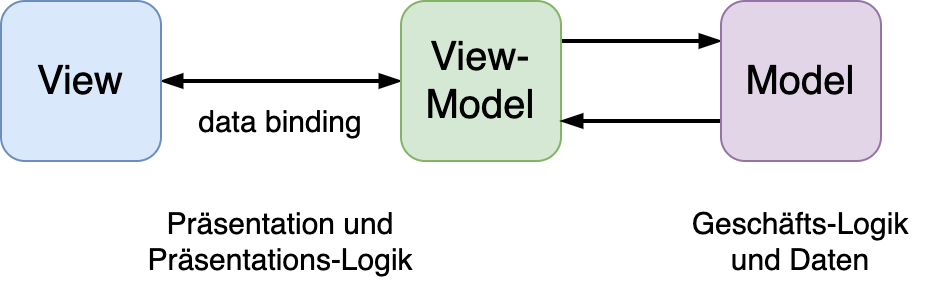
\includegraphics[width=0.7\textwidth]{img/mvvm}
    			\caption{Schematische Darstellung des Model-View-ViewModel Konzepts}
    			\label{fig:mvvm}
    		\end{figure}
    		
		\vspace{-5mm}
		\paragraph*{Redux.js}
			Redux.js ist eine Bibliothek\footurl{Redux.js Github Repository -}{https://github.com/reduxjs/redux} für die Programmiersprache JavaScript und stellt einen sogenannten vorhersehbaren Zustandscontainer\footurl{Redux Core Concepts -}{https://redux.js.org/introduction/core-concepts} für JavaScript-Anwendungen bereit. In diesem Container wird der Zustand der gesamten Anwendung in einem sogenannten Objektbaum gespeichert. Dieser Baum ist mit der Ordner-Struktur von Windows vergleichbar. Es gibt einen Wurzel-Ordner, in dem wiederum Ordner oder aber auch Dateien enthalten sind. Im Zustandscontainer bezeichnet man die Ordner als States bzw. auf deutsch Zustände. Die Dateien sind einfache Daten, die unteranderem auf der Benutzeroberfläche angezeigt werden sollen. Diese Aufteilung in die States ist dazu gedacht, jeder View nur die wirklich benötigten Daten bereitzustellen. Diese Struktur erleichtert das Testen oder Untersuchen der Anwendung und ermöglicht es, durch Hinzufügen eines neuen States den aktuellen Entwicklungsstand der Anwendung beizubehalten und dadurch den Entwicklungsprozess zu beschleunigen. \\
			Ein weiteres wichtiges Prinzip\footurl{Redux Three Principles -}{https://redux.js.org/introduction/three-principles} von Redux ist, dass die Daten in den States schreibgeschützt sind. Die einzige Möglichkeit den Zustand bzw. die Daten zu ändern, besteht darin, eine Aktion auszulösen. Die Aktion beschreibt, wie der State und dessen Daten sich ändert. Dadurch wird sichergestellt, dass weder die Views noch Netzwerk-Rückrufe jemals direkt den Zustand ändern können. Stattdessen bringen sie nur die Absicht zum Ausdruck, den State zu verändern und lösen eine Aktion aus, die die Änderung für sie vornimmt. Da alle Aktionen zentralisiert sind und eine nach der anderen in einer strikten Reihenfolge erfolgen, gibt es weniger Programmfehlerquellen.

	\section{Entwurf und Design}\label{sc:entwurfunddesign}
		In der Entwurfsphase wird normalerweise über die Datenhaltung, die Verteilung des Software-Systems im Netz und die Benutzeroberfläche entschieden\footurl{Vorlesung 9, Folie 27 aus Softwaretechnik Grundlagen von Prof. Dr.-Ing. Wilfried Schubert (2019) -}{https://www.staff.hs-mittweida.de/~wschub/intranet/ss19/Fach_SWT/Fach_SWT_Zeitplan.htm}. Jedoch standen diese Grundsatzentscheidungen schon zu Beginn des Praktikums durch die Kenntnisse von Tobias Kallauke und dem Verfasser fest. Zur Datenspeicherung verwendet der Server PostgreSQL\footurl{PostgreSQL Internetseite -}{https://www.postgresql.org/}, eine relationale Datenbank. Zum Speichern der Bilder wird die Server-Verzeichnisstruktur genutzt. In der App hingegen werden keine Daten persistent gespeichert. Durch die Aufteilung von App und Server handelt es sich um eine sogenannte Client-Server-Architektur und für die Benutzeroberfläche der iOS-App wird, wie schon erwähnt, das deklarative SwiftUI verwendet. Weitere Informationen zum Entwurf der Server-Architektur und der Android-App befinden sich im Praktikumsbericht von Tobias Kallauke.
		
		Zur Definition einzelner Teil-Workflows, die zusammenhängende Aufgaben umfassen, wurden Flussdiagramme und schriftliche Zustandsautomaten angefertigt (siehe \autoref{ch:workflow}). Diese Modelle halfen dabei Views zu entwickeln und deren Design festzulegen. Das Aussehen der App sollten sich jedoch im Laufe der Zeit noch ändern, da erst einmal die Umsetzung des Konzepts im Vordergrund stand.

		Ausgehend vom Design und den Teil-Workflows entstand ein grobes Konzept zur Handhabung der Daten innerhalb der App. Da SwiftUI das Entwurfsmuster MVVM umsetzt, wird eine Struktur für das ViewModel und für den Datenfluss der asynchronen Server-Rückrufe benötigt. Die Struktur-Entwicklung erwies sich bereits während des ersten Prototyps als problematisch. Denn auch bei steigender Komplexität sollte das ViewModel noch übersichtlich bleiben, um eine schnelle Weiterentwicklung zu gewährleisten. Bei der Suche nach einer besseren Lösung wurde die JavaScript-Bibliothek Redux.js zur Verwaltung von Zustandsinformationen in Webanwendungen gefunden.  

		Das Konzept von Redux hilft komplexe Views mit vielen Daten schnell und einfach zu implementieren. Somit werden Server-Antworten und zwischengespeicherte Daten sowie lokal erstellte Daten, die noch nicht auf dem Server gespeichert wurden, strukturiert und zentral abgelegt. Das erleichtert nicht nur das Wiederverwenden von Daten, sondern reduziert die Wiederholung von Server-Aufrufen. Zudem ermöglicht Redux durch die modulare Aufteilung des State-Containers eine schnelle Weiterentwicklung der App, trotz steigender Komplexität. Zudem stellten die Vorteile hinsichtlich des Testens und Untersuchens der App, das schnelle Auffinden von Fehlern in Aussicht. Es erschien nun möglich, trotz begrenzter Praktikumszeit, den Prototyp möglichst fehlerfrei und weit zu entwickeln.

%%%%%%%%%%%%%%%%%%%%%
		Daher lag es nah die wesentlichen Konzepte von Redux umzusetzen und einen Redux ähnlichen State Container, als ViewModel zu implementieren. Aus der Definition von Teil-Workflows sollte der Container oder auch Store genannt mindestens 5 States haben: 
		\vspace{-5mm}
		\begin{itemize}
			\item Für Authentifizierung sowie Registrierung,
			\item für das Anlegen von Scan-Vorlagen und Speichern der Zwischenergebnisse,
			\item für das Ausführen von Server-Aufrufen zum Speichern und Abrufen von Vorlagen, 
			\item für die Steuerung des Workflows bzw. den stellvertretenden Views sowie
			\item für sonstige Daten, die sehr häufig verwendet werden.
		\end{itemize}
		
		\begin{figure}[h!]
			\centering
			\begin{subfigure}[t]{0.48\textwidth}
				\centering
				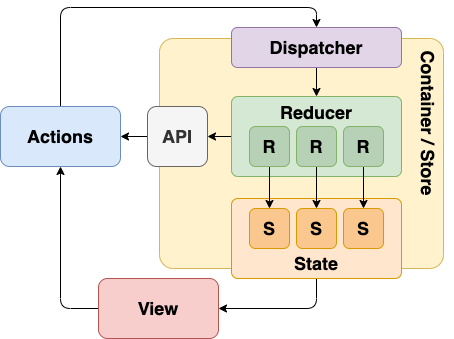
\includegraphics[width=\textwidth]{img/redux.png}
				\caption{Schema der Documenten-Scanner Architektur}
				\label{fig:redux}
			\end{subfigure}
			\begin{subfigure}[t]{0.48\textwidth}
				\centering
				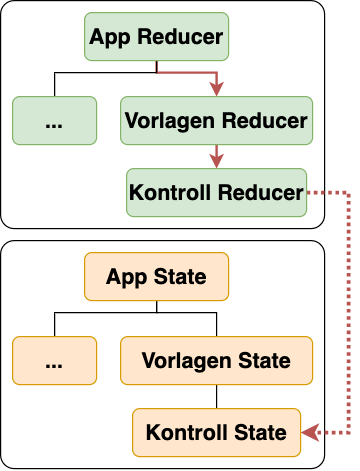
\includegraphics[height=0.9\textwidth]{img/tree_example.png}
				\caption{Beispiel für einen Reducer- und State-Objektbaum}
				\label{fig:tree}
			\end{subfigure}
			\caption{Architektur Schemata}
		\end{figure}
		
		Das Schema \ref{fig:redux} zeigt, die in der App umgesetzte Struktur. Über eine View (rot) können Aktionen (blau) aufgerufen werden. Diese gelangen zuerst in einen sogenannten Dispatcher (lila), welcher als Verteiler dient. Anhand der Art einer Aktion, wird der entsprechende Reducer (grün) vom Dispatcher beauftragt, die Aktion auszuführen. Jeweils ein Reducer ist nur für eine Aktions-Art zuständig. In \autoref{fig:tree} ist eine Schachtelung von Reducern (grün) zu sehen. Ebenfalls können Aktions-Arten ineinander geschachtelt werden. Das hat den Hintergrund, dass die States wie ein Objektbaum aufgebaut sind. So hat jeder State seinen eigenen Reducer und eigene Aktionen, was für die oben erwähnte Modularität sorgt. Muss beispielsweise eine Änderung im Kontroll-Mechanismen-State (siehe Kontroll-State in \ref{fig:tree}) vorgenommen werden, wird die Haupt-Aktion in einer Kontroll-Mechanismen-Reducer-Aktion geschachtelt und diese wiederum in einer Vorlagen-Reducer-Aktion. Zum Ausführen der Haupt-Aktion, werden zuvor die entsprechenden Reducer die Schachtelung von außen nach innen auflösen. Nachdem die Aktion ausgeführt und eine State-Änderung herbeigeführt wurde, aktualisiert sich durch data binding von MVVM die View. Speziell werden alle Views, die eine Bindung zu dem jeweiligen Datum im State haben, über die Änderung benachrichtigt und daraufhin aktualisieren diese ihre Benutzeroberfläche.

		Ein weiterer wichtiger Bestandteil der Architektur sind die Server-Aufrufe. Für diese gibt es einen eigenen Reducer und eigene Schnittstellen. Diese Schnittstellen sind in der \autoref{fig:redux} grau markiert und mit API \nomenclature{API}{application programming interface, deutsch: Programmierschnittstelle} beschriftet. Ihre Besonderheit besteht darin, selbst Aktionen an den Container zu senden. Beispielsweise löst der Benutzer die Aktion aus, alle Vorlagen vom Server zu laden. Diese Aktion gelangt über den vorgesehenen Reducer zu der API-Schnittstelle. Dort wird ein entsprechender Server-Aufruf gestartet und auf den Server-Rückruf gewartet. Sobald die Antwort des Servers angekommen ist, wird diese mit Hilfe einer Aktion zurück zum Container gesendet. Dort verarbeitet ein entsprechender Reducer eventuelle Fehler oder die heruntergeladenen Vorlagen.
		
	\section{Implementierung}\label{sc:implementierung}
		Zur Realisierung der entworfenen Systemkomponenten wurde ausschließlich, die von Apple entwickelte IDE\nomenclature{IDE}{integrated development environment, deutsch: Integrierte Entwicklungsumgebung} Xcode\footurl{Xcode Internetseite -}{https://developer.apple.com/xcode/}, verwendet. Diese stellt virtuelle iOS oder iPadOS Geräte zur Verfügung, auf denen die App getestet werden kann. Diese Simulatoren bieten unteranderem auch die Möglichkeit, die Anwendung schnell auf verschiedenen Betriebssystem-Versionen zu testen. Auch ist das Testen der App auf echten Geräten durch Xcode möglich, was bei der Entwicklung unumgänglich war. Grund dafür ist die Benutzung der Kamera, die bei den Simulatoren zu gewollten Abstürzen führt, da diese keinen Zugriff auf ein Kamerasystem besitzen.
		
		Die App ist ausschließlich in der Programmiersprache Swift geschrieben. Neben den Frameworks SwiftUI, Vision und VisionKit von Apple wurde das Framework Kingfisher\footurl{Kingfisher GitHub Repository -}{https://github.com/onevcat/Kingfisher}, zum Downloaden und Cachen von Bildern verwendet. Das Vision-Framework führt Gesichts-, Text- und Barcode-Erkennung, Bildregistrierung und allgemeine Merkmalsverfolgung durch. Jedoch wurde in der App nur die integrierte Texterkennung benutzt. Es ist aber anzunehmen, dass zur Dokumenten-Erkennung  Algorithmen aus Vision von VisionKit verwendet werden. Für mehr Informationen über die Frameworks SwiftUI und VisionKit siehe in \autoref{sc:analyse}.
		
		Zum Einrichten und Testen des Backends wurde außerdem Visual Studio Community bzw. Visual Studio Code\footurl{Visual Studio Internetseite -}{https://visualstudio.microsoft.com/de/} mit dem REST Client Plugin\footurl{REST Client Repository -}{https://github.com/Huachao/vscode-restclient} verwendet. Das Backend konnte als lokaler Server auf dem Entwicklungscomputer gestartet und im lokalen Netzwerk aufgerufen werden. Für die Verwaltung der PostgreSQL-Datenbank bot sich PgAdmin4\footurl{PgAdmin Internetseite -}{https://www.pgadmin.org/} an. Damit ist es möglich, einzelne Einträge oder auch ganze Tabellen der Datenbank zu bearbeiten.

		\subsection{Registrieren und Anmelden}
			Die E-Mail-Textfelder besitzen, wie auch das Passwortfeld der Anmeldung eine AutoFill-Funktion. Dadurch kann die App Registrier- und Anmeldedaten vorschlagen und automatisch in die entsprechenden Felder einsetzten. Im dritten Bild \ref{fig:anmelden} ist das anhand des \glqq Passwörter\grqq -Knopfes über der Tastatur zu sehen. Außerdem sind alle Passwortfelder gesichert, wodurch der Inhalt zum Schutz der Privatsphäre standardmäßig ausgeblendet und mit Punkten ersetzt wird. Aufgrund der Sicherheitsstandards von iOS sind die Punkte auf der Bildschirmaufnahme \ref{fig:register} nicht zu sehen. Durch Berühren des Auges neben dem Textfeld kann der Inhalt ein- und ausgeblendet werden. Zusätzlich validieren alle Textfelder ihren Inhalt mithilfe von regulären Ausdrücken. Beispielsweise muss ein Passwort aus 8 Zeichen bestehen und zwei von den drei folgenden Eigenschaften erfüllen:
			\vspace{-5mm}
			\begin{enumerate}
				\item Es ist mindestens ein Sonderzeichen enthalten.
				\item Es ist mindestens ein Großbuchstabe enthalten.
				\item Es ist mindestens eine Zahl enthalten.
			\end{enumerate}
			\vspace{-5mm}
			Die Validierung ist jedoch nicht standardmäßig, sondern wurde selbst entwickelt.

			
		\begin{figure}[th!]
    		\centering
   			\begin{subfigure}[t]{0.3\textwidth}
       			\frame{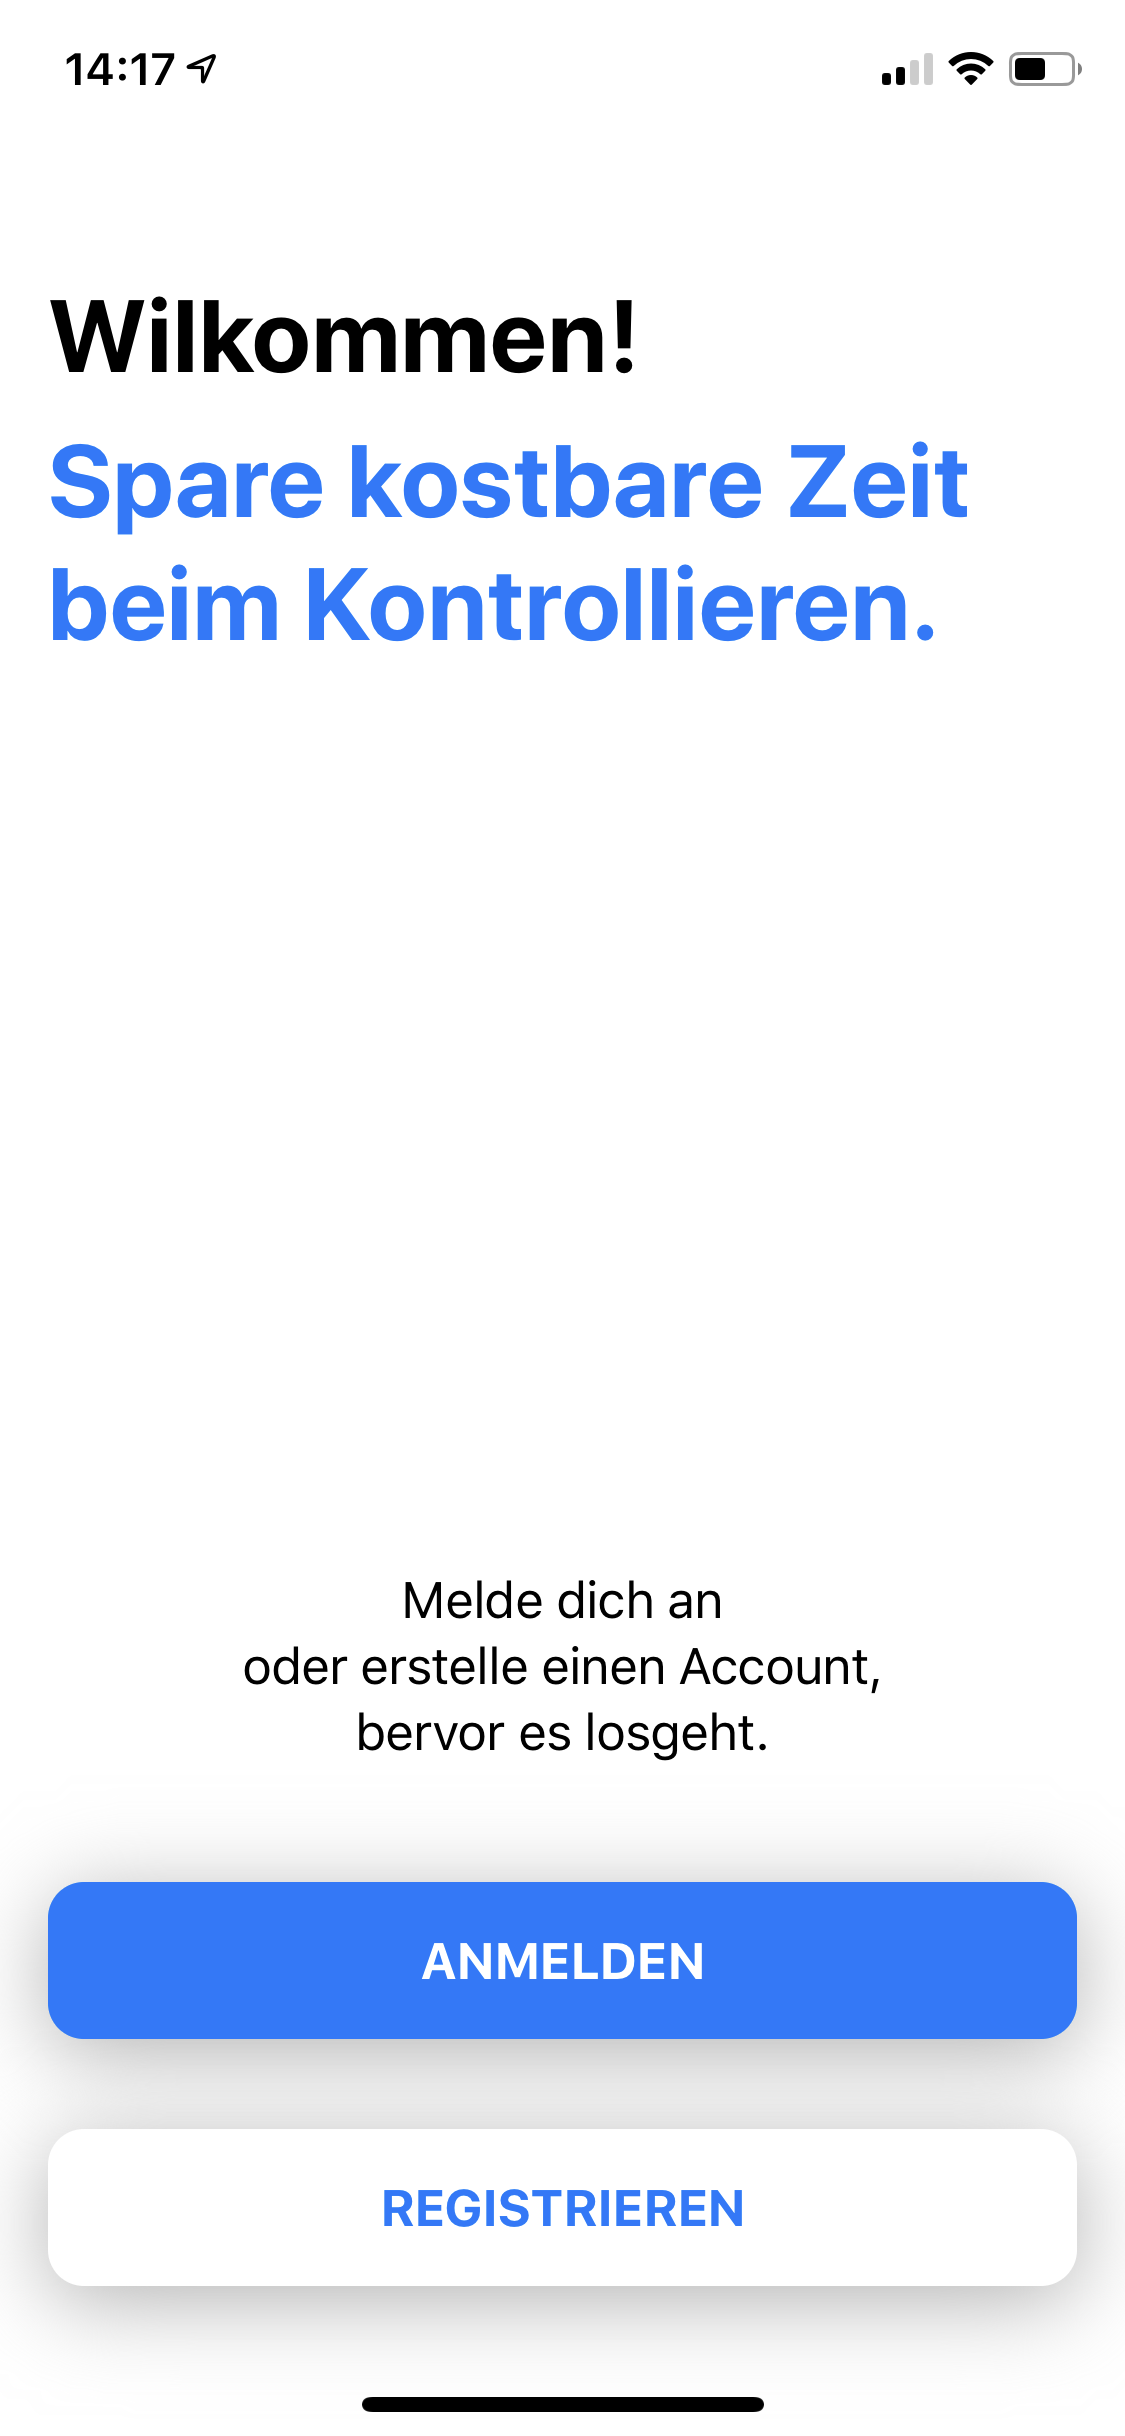
\includegraphics[width=0.96\textwidth]{img/1willkommen.png}}
       			\caption{Willkommen View}
       			\label{fig:willkommen}
       		\end{subfigure}
    		\begin{subfigure}[t]{0.3\textwidth}
        		\frame{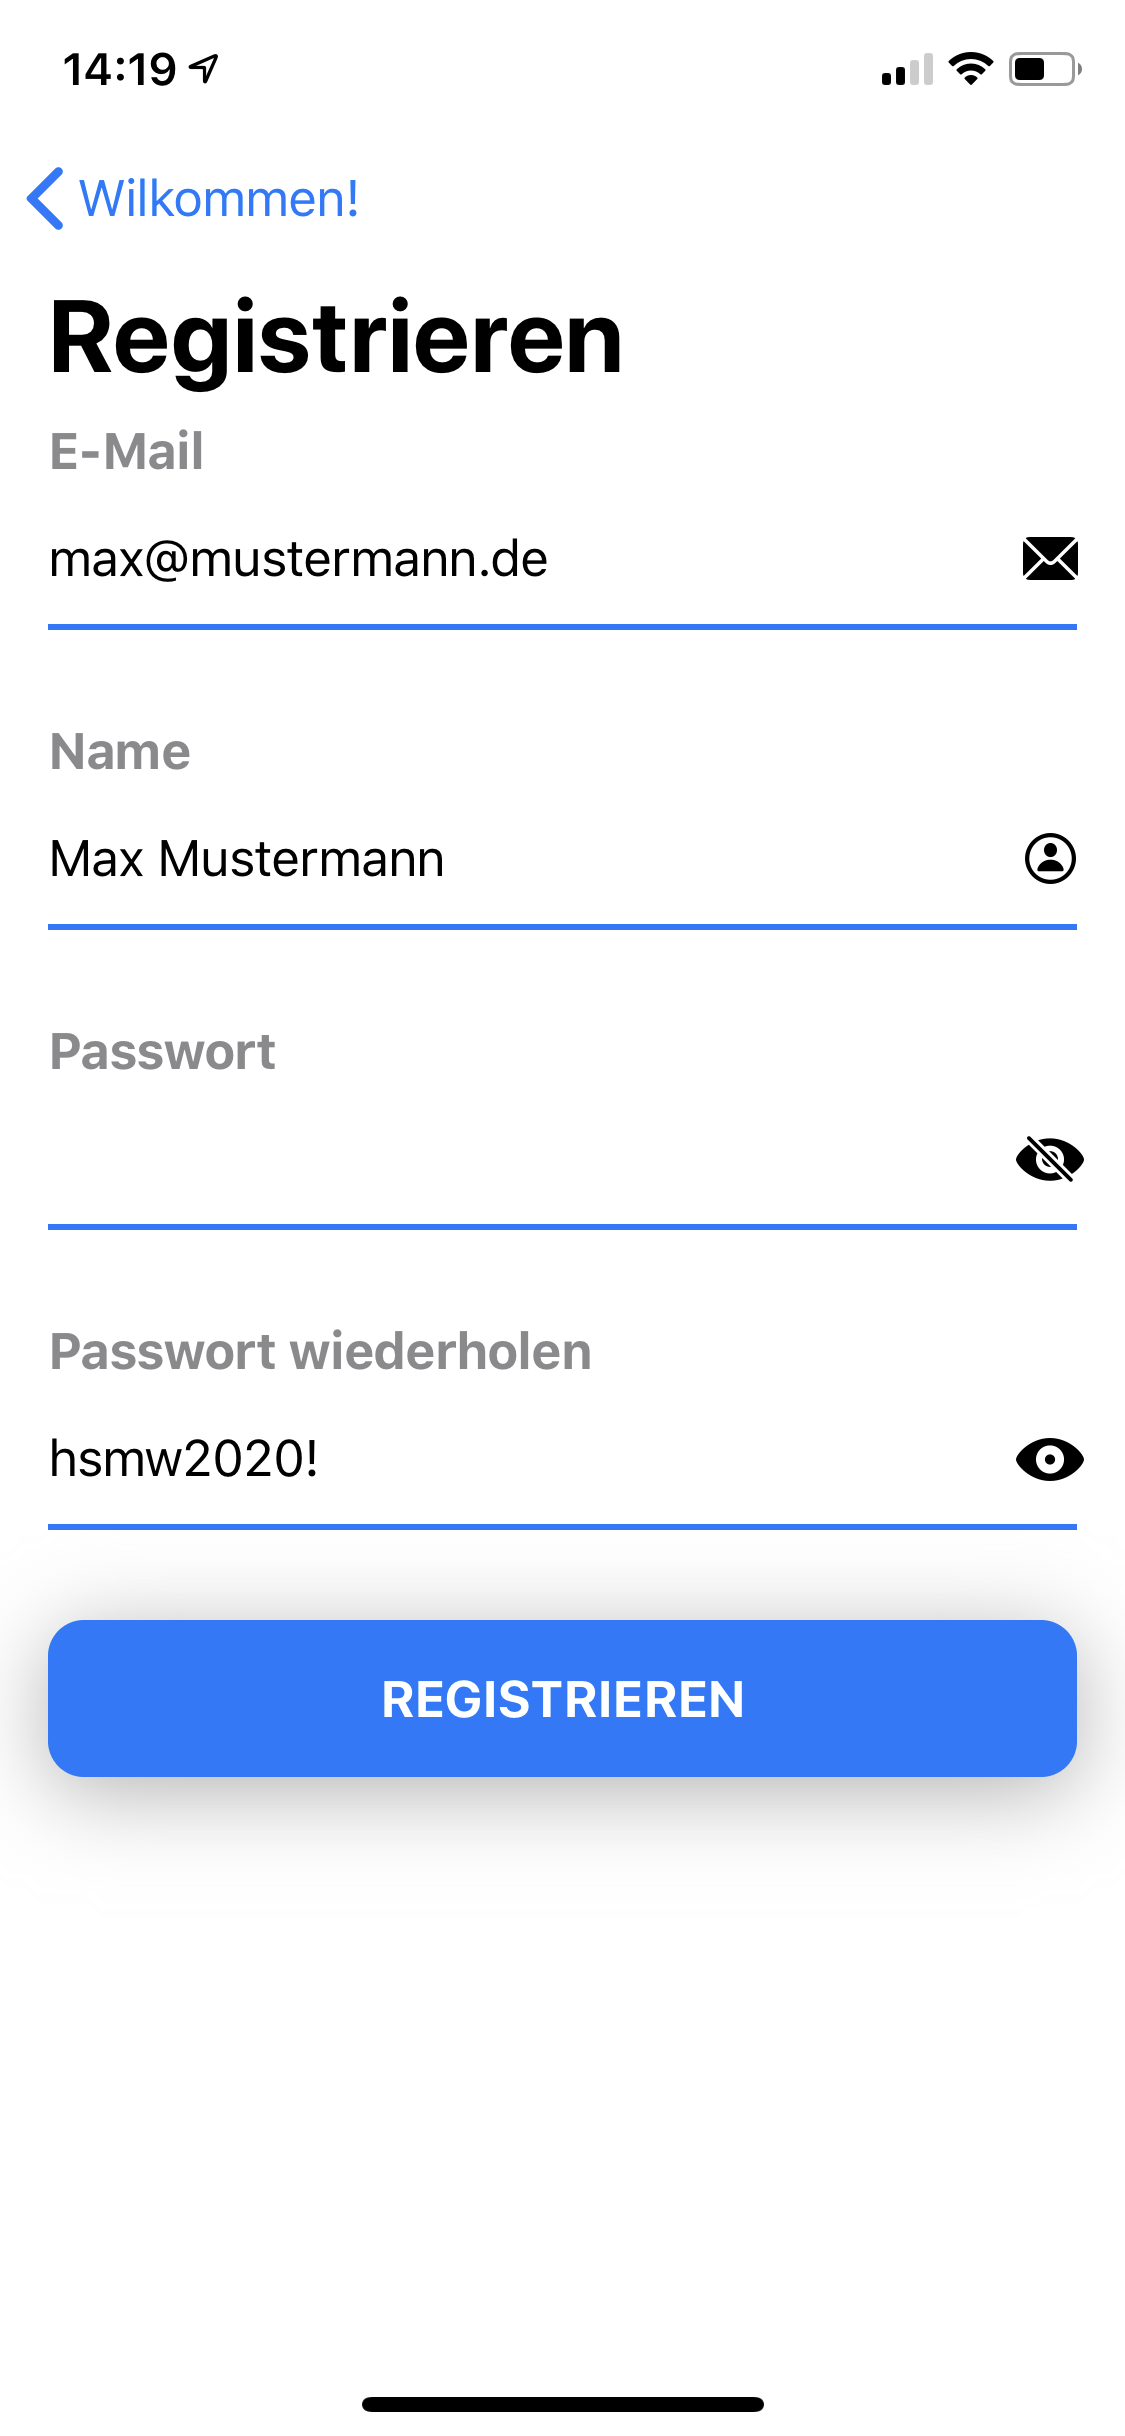
\includegraphics[width=0.96\textwidth]{img/7reg_full_see.png}}
      			\caption{Registrierung mit sicheren Eingabefeldern}
       			\label{fig:register}
   			\end{subfigure}
   			\begin{subfigure}[t]{0.3\textwidth}
      			\frame{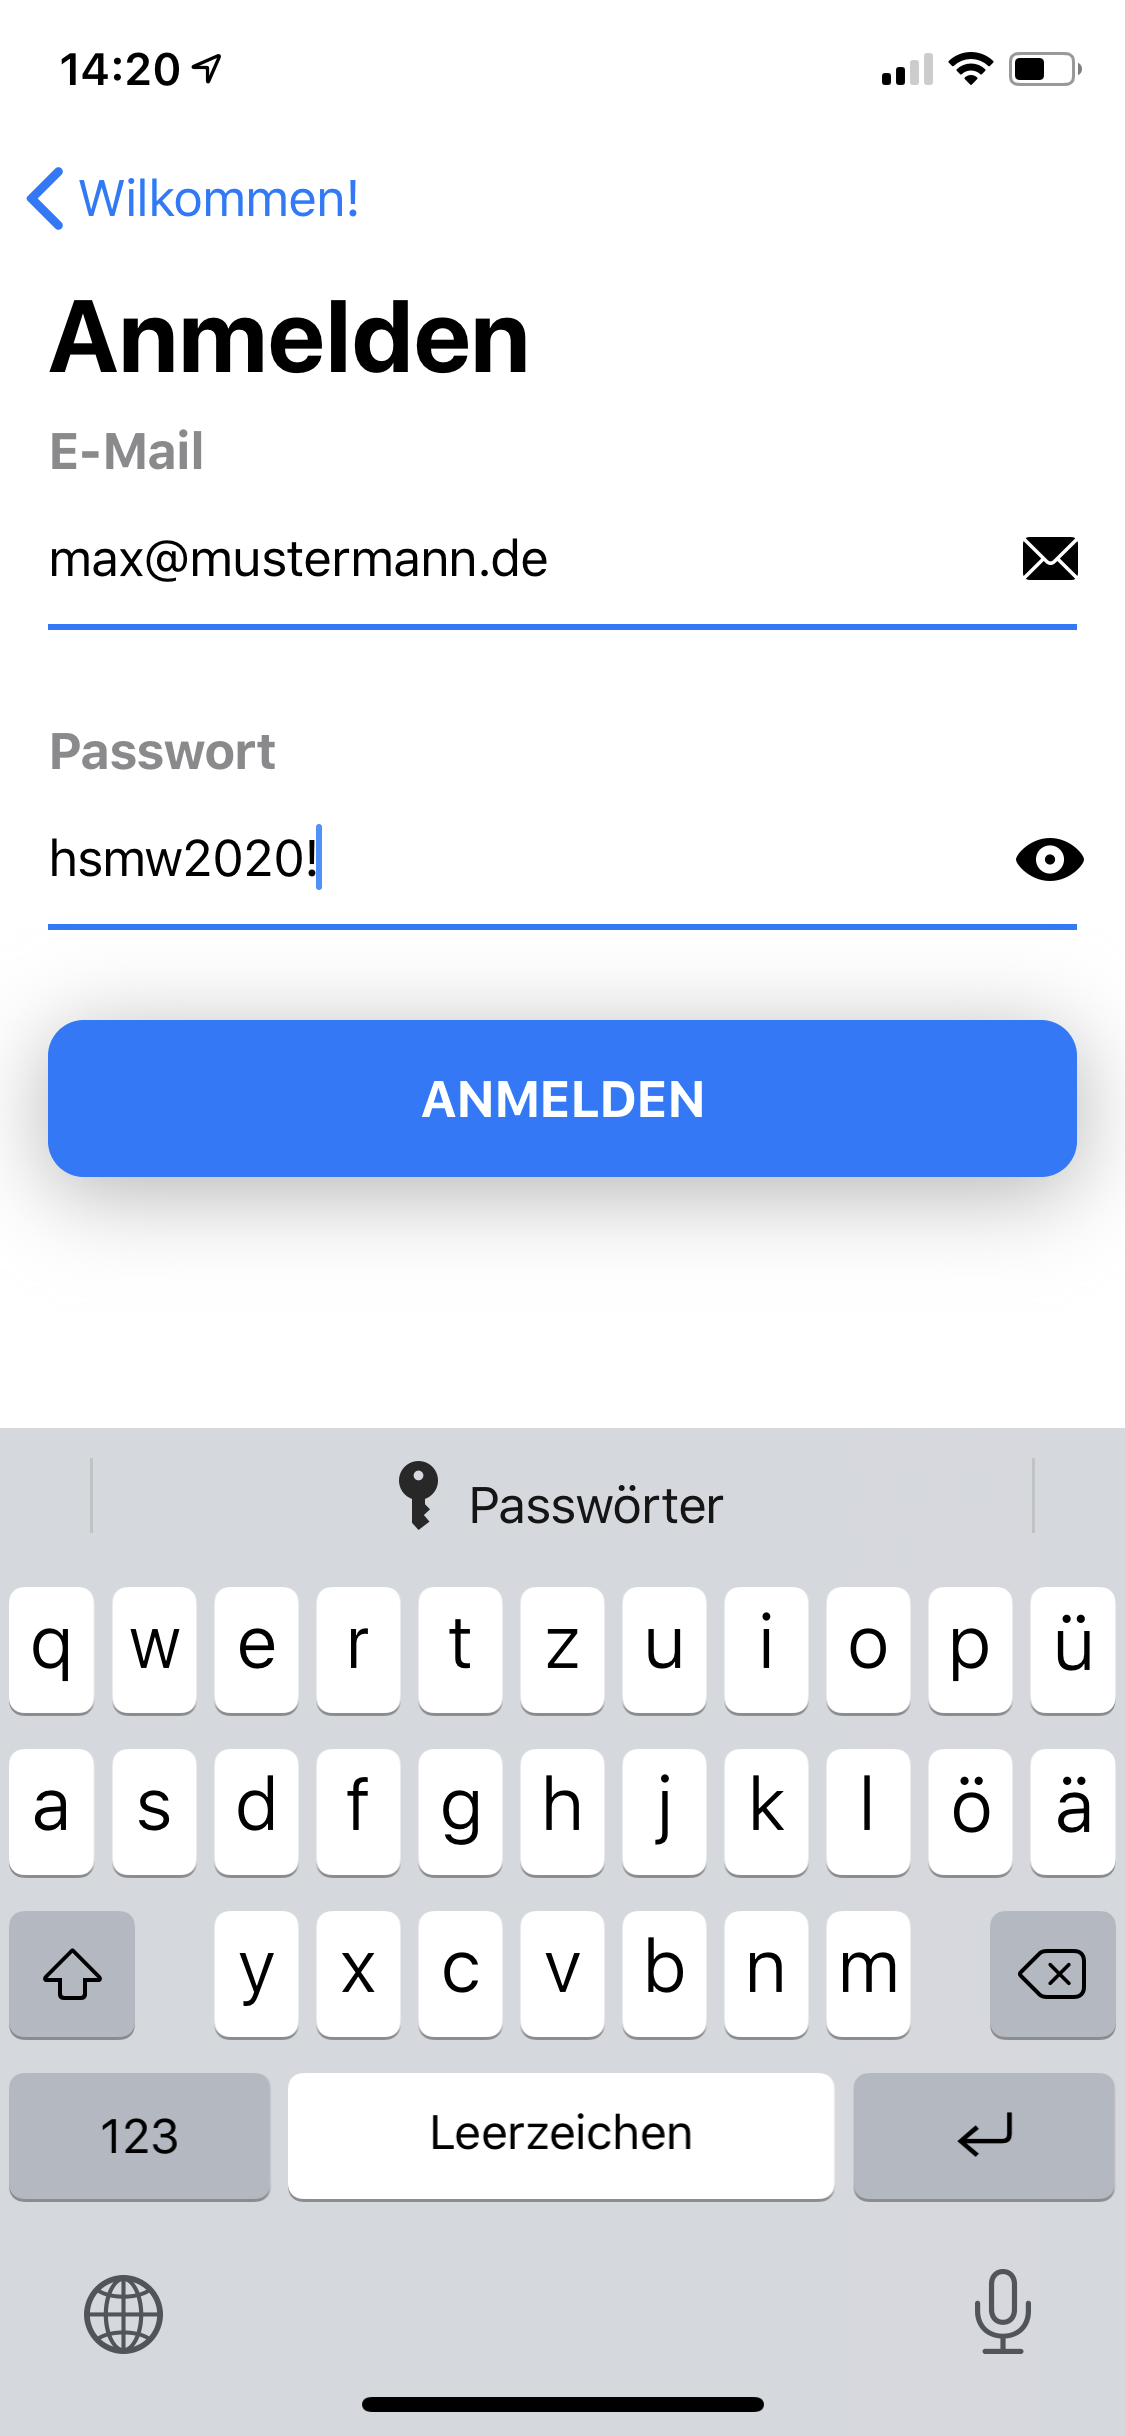
\includegraphics[width=0.96\textwidth]{img/12an_full_pass.png}}
        		\caption{Anmeldung mit AutoFill-Funktion}
	       		\label{fig:anmelden}
    		\end{subfigure}
   			\caption{Willkommen- Registrier- und Anmelde-View}\label{fig:start}
		\end{figure}	
		
		\subsection{Scan-Vorlagen erstellen und speichern}
			Bei der Implementierung des ersten Arbeitsschrittes der Scan-Vorlagen wurde das Flussdiagramm \ref{fig:erstellen_flow}, welches im \autoref{ch:workflow} zu finden sind, benutzt.
			
			\subsubsection*{Scan-Vorlage erstellen}
				Zu Beginn sind ein Name und eine Beschreibung der Vorlage anzugeben (siehe \ref{fig:v2}), um im Anschluss die Fotos aufzunehmen. Bei der Kamera-View (siehe \ref{fig:v3}) handelt es sich um die Scan-View des Frameworks VisionKit. Mithilfe von Kantenerkennung und anderen Algorithmen, die Tobias Kallauke in seinem Bericht beschreibt, wird das Dokument, sobald es erkannt ist, automatisch fotografiert. Das Dokument wird in Echtzeit aus dem Bild ausgeschnitten und gerade gezogen. Ein manuelles Auslösen des Fotos und Anpassen der Dokumentenkanten im Bild, ist ebenfalls möglich. Zugleich werden alle erstellten Bilder in einer Gruppe gesammelt. Diese können vor dem Abspeichern angeschaut und nochmals bearbeitet werden. Die \autoref{fig:klausur} entstand durch diesen Prozess. 

				
			\begin{figure}[h!]
    			\centering
    			\begin{subfigure}[t]{0.3\textwidth}
        			\frame{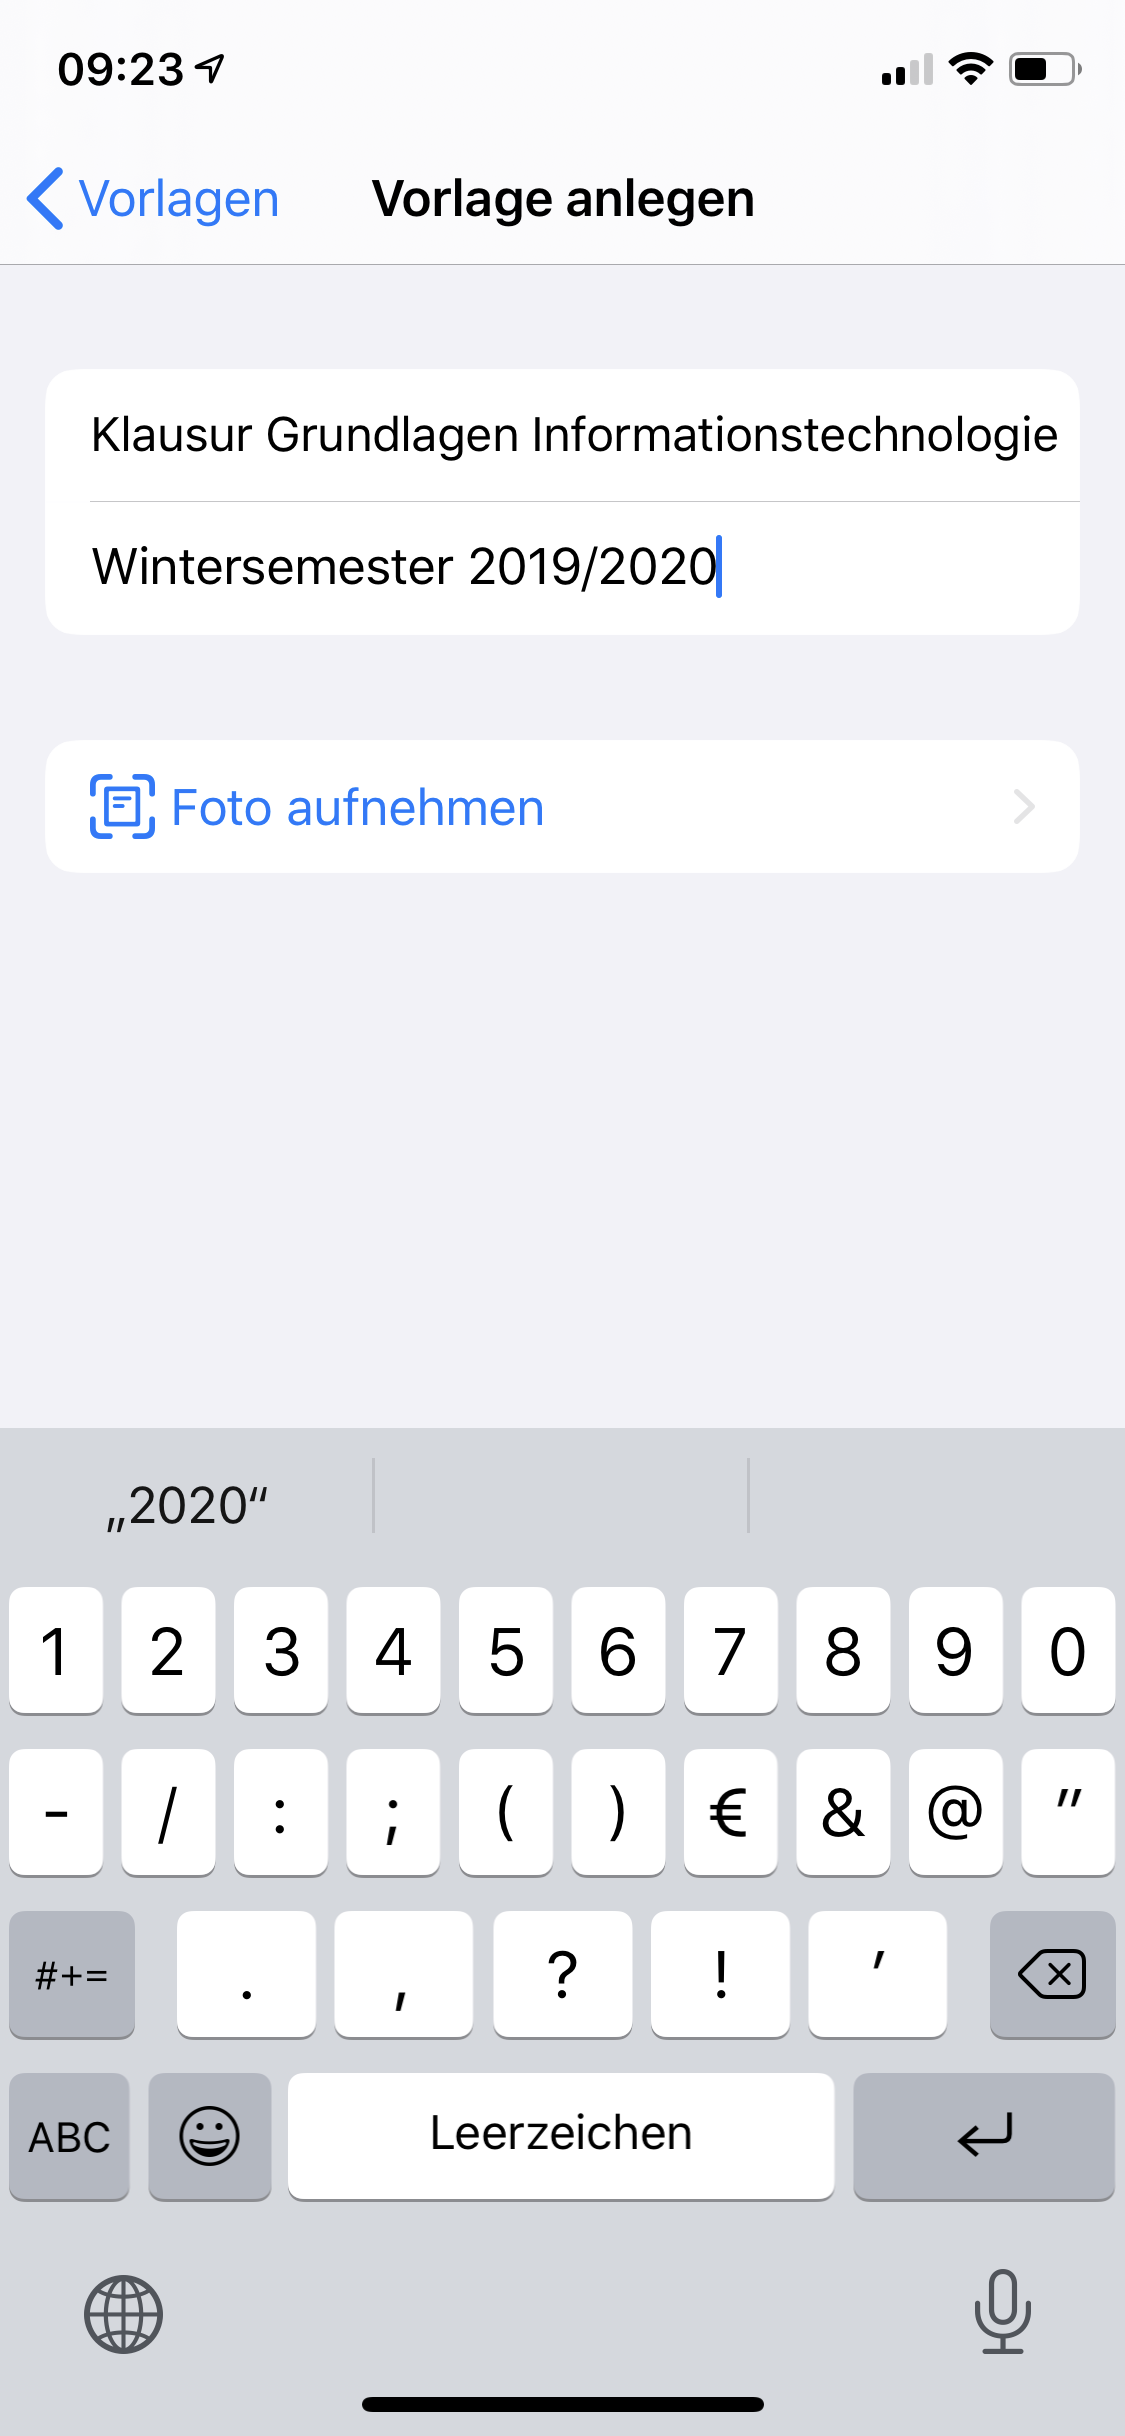
\includegraphics[width=0.96\textwidth]{img/V2}}
        			\caption{View zum Anlegen einer Vorlage}
        			\label{fig:v2}
    			\end{subfigure}
    			\begin{subfigure}[t]{0.3\textwidth}
        			\frame{\includegraphics[width=0.96\textwidth]{img/V3}}
        			\caption{Kamera- bzw. Scan-View mit Dokumenten-Erkennung}
        			\label{fig:v3}
    			\end{subfigure}
    			\begin{subfigure}[t]{0.3\textwidth}
       				\frame{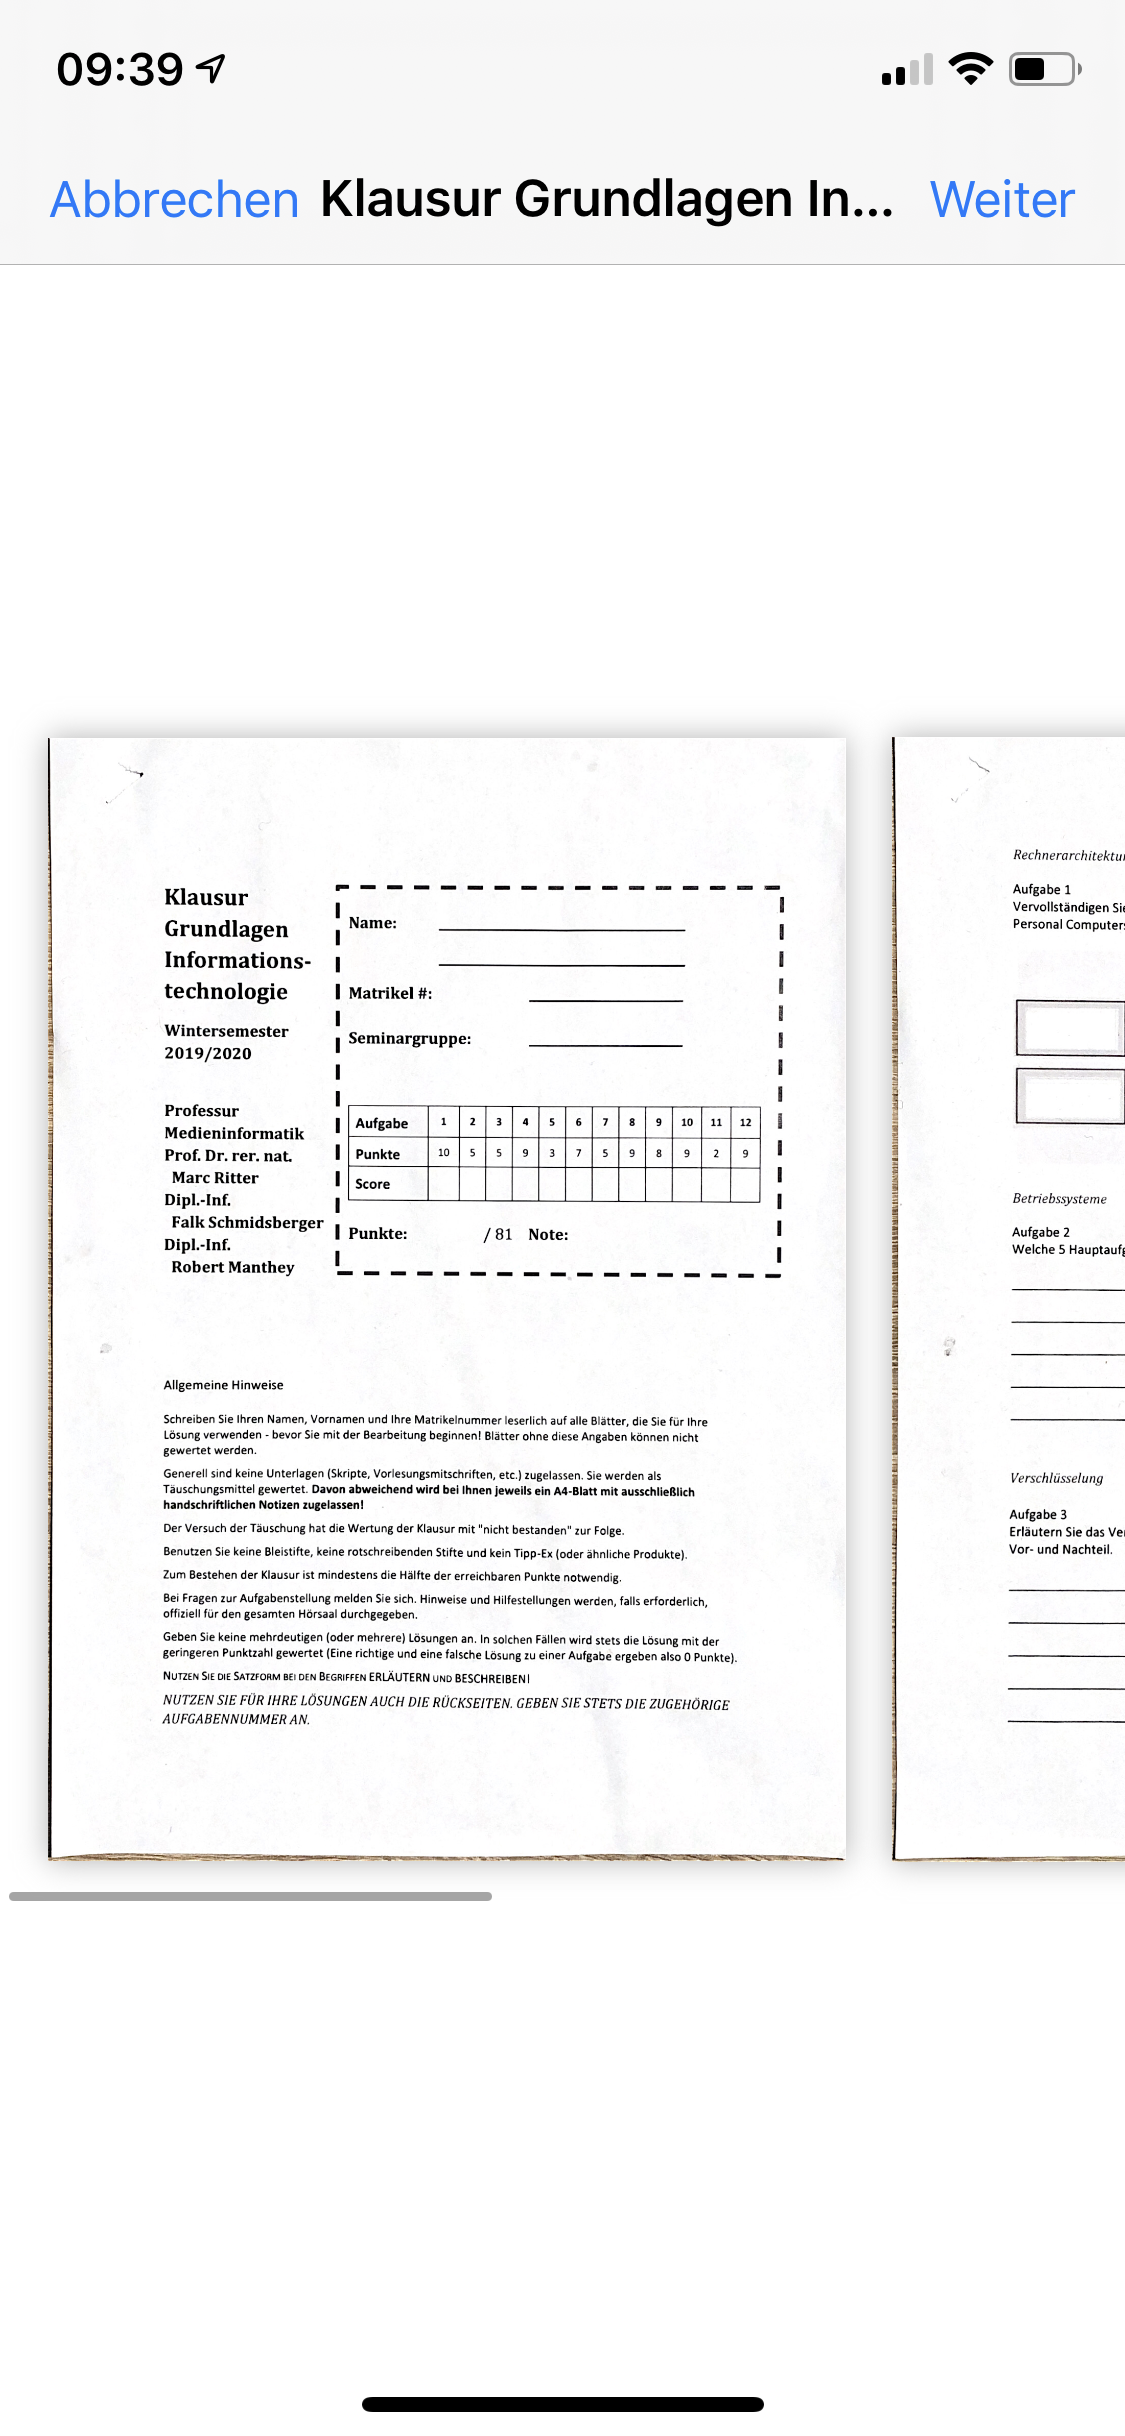
\includegraphics[width=0.96\textwidth]{img/V4}}
        			\caption{Seiten-Auswahl-View}
        			\label{fig:v4}
    			\end{subfigure}
    			\caption{Die ersten Views zur Erstellung einer Scan-Vorlage}\label{fig:erstellung1}
			\end{figure}
			
			\subsubsection*{Regionen erstellen}
				Im Anschluss sind die Regionen auf den Dokumentenseiten zu markieren, deren Inhalt beim Einscannen digitalisiert werden soll. Dafür wird zunächst die gewünschte Seite aus einer Übersicht (siehe \ref{fig:v4}) ausgewählt. Anschließend ist eine Vorschau der Seite mit allen eingetragenen Regionen zu sehen (siehe \ref{fig:v8} bzw. \ref{fig:v9}). Über einen Button können weitere Regionen hinzugefügt werden. Dazu muss ein Name (siehe \ref{fig:v5}) und ein Datentyp (siehe \ref{fig:v6}) festgelegt werden. Sobald die Eigenschaften der Region definiert sind, muss diese Region auf dem Bild markiert werden. Dazu zieht man mit einem Finger ein Rechteck über die gewünschte Region (siehe \ref{fig:v7}). Zudem kann an die Seite heran- oder herausgezoomt werden, um beispielsweise kleine Regionen zu markieren. Dieses Vorgehen muss anschließend für alle benötigen Regionen auf den jeweiligen Seiten wiederholt werden.
 
				\begin{figure}[h!]
    				\centering
    				\begin{subfigure}[t]{0.3\textwidth}
        				\frame{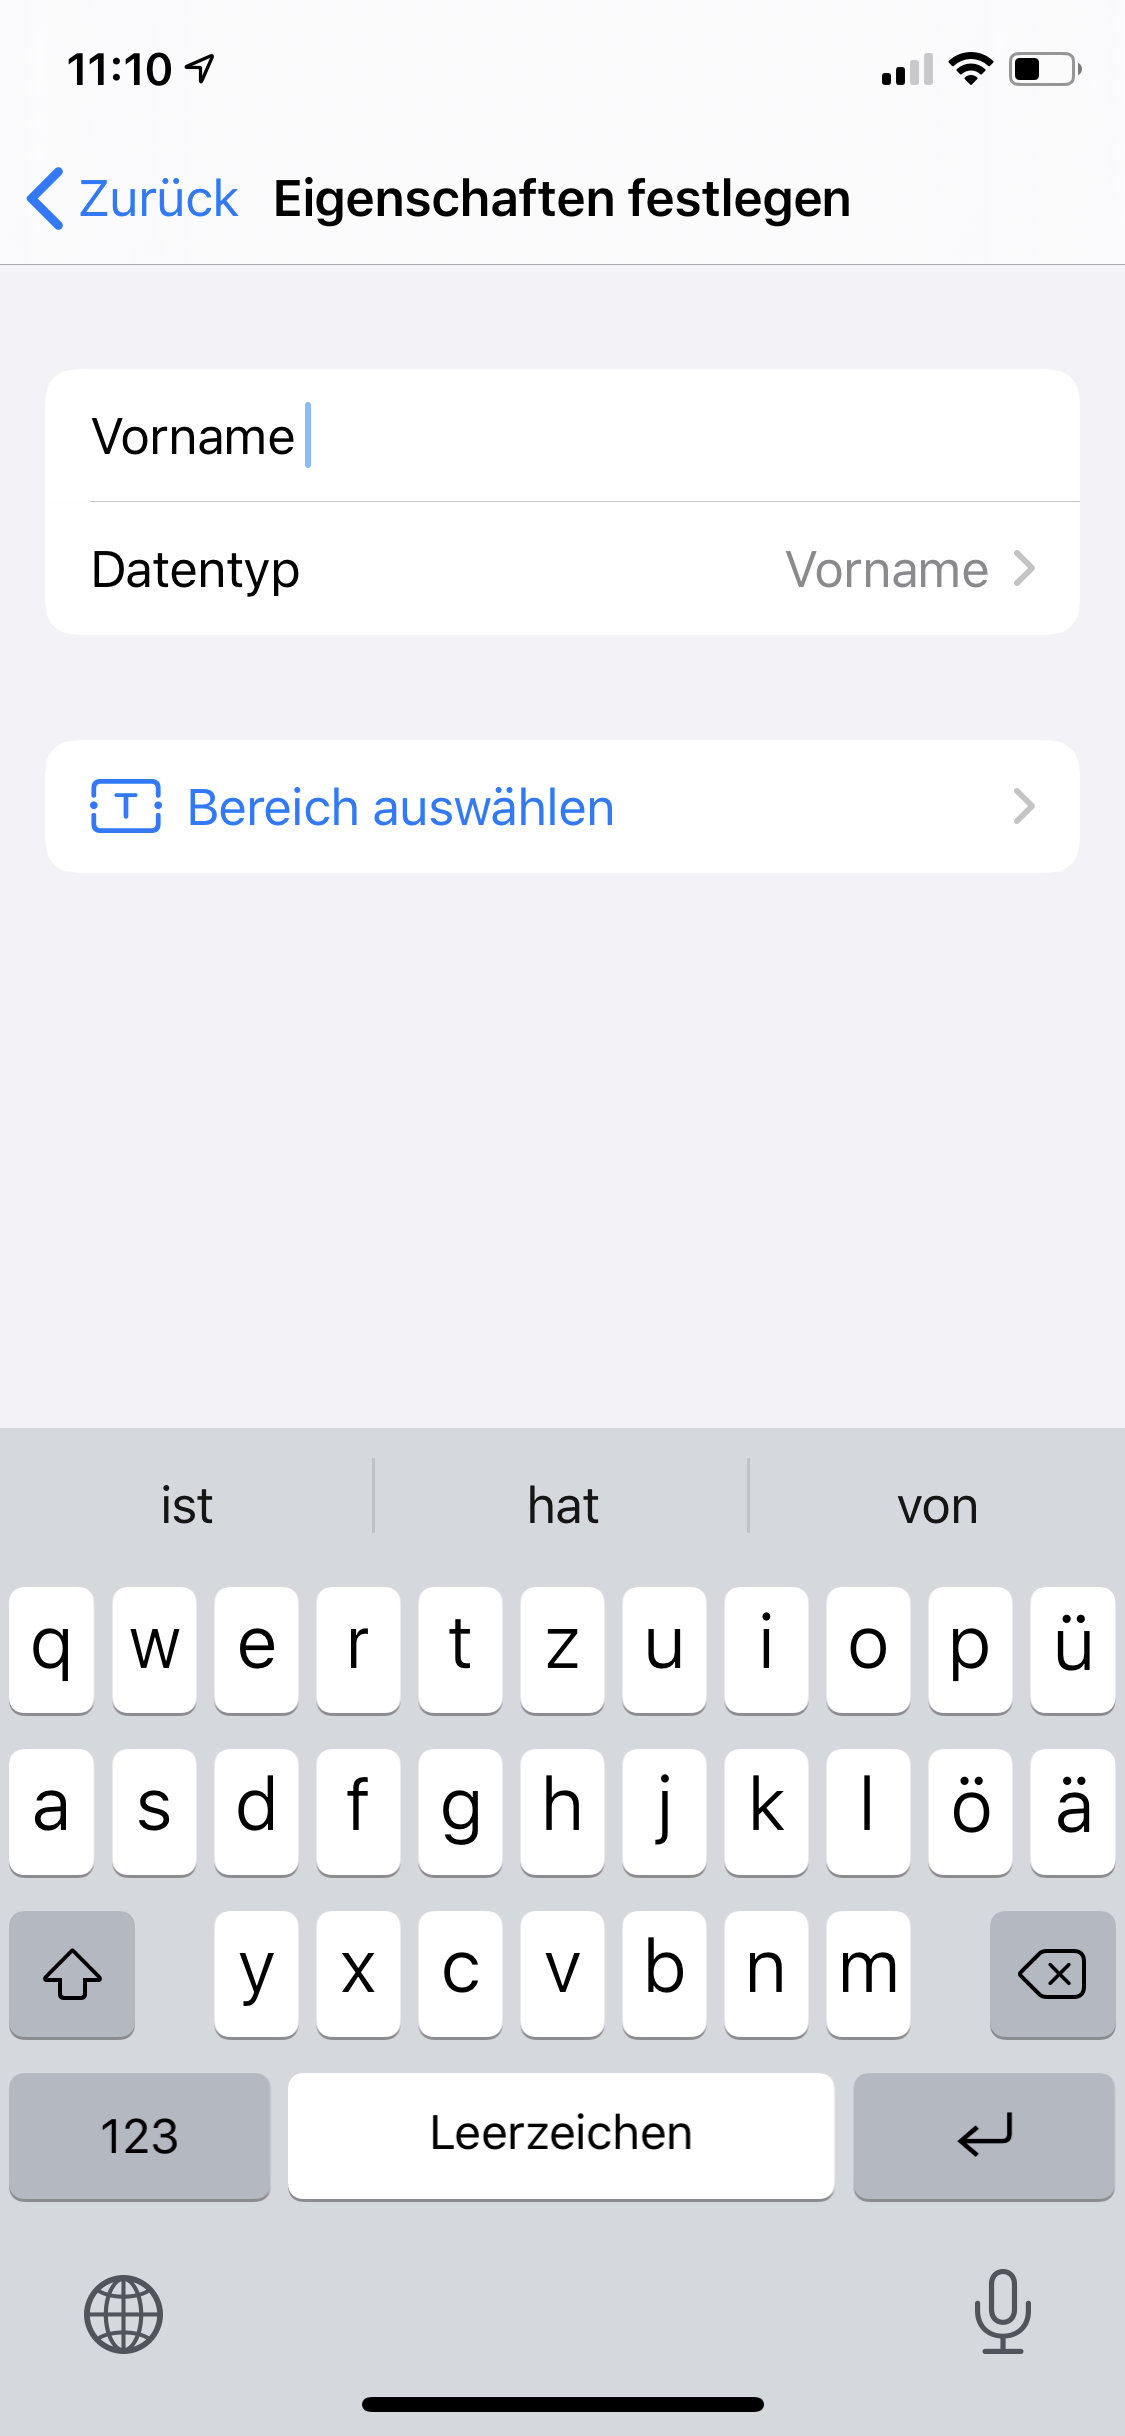
\includegraphics[width=0.96\textwidth]{img/V5}}
        				\caption{View zum Festlegen von den Regionen Eigenschaften}
        				\label{fig:v5}
    				\end{subfigure}
    				\begin{subfigure}[t]{0.3\textwidth}
        				\frame{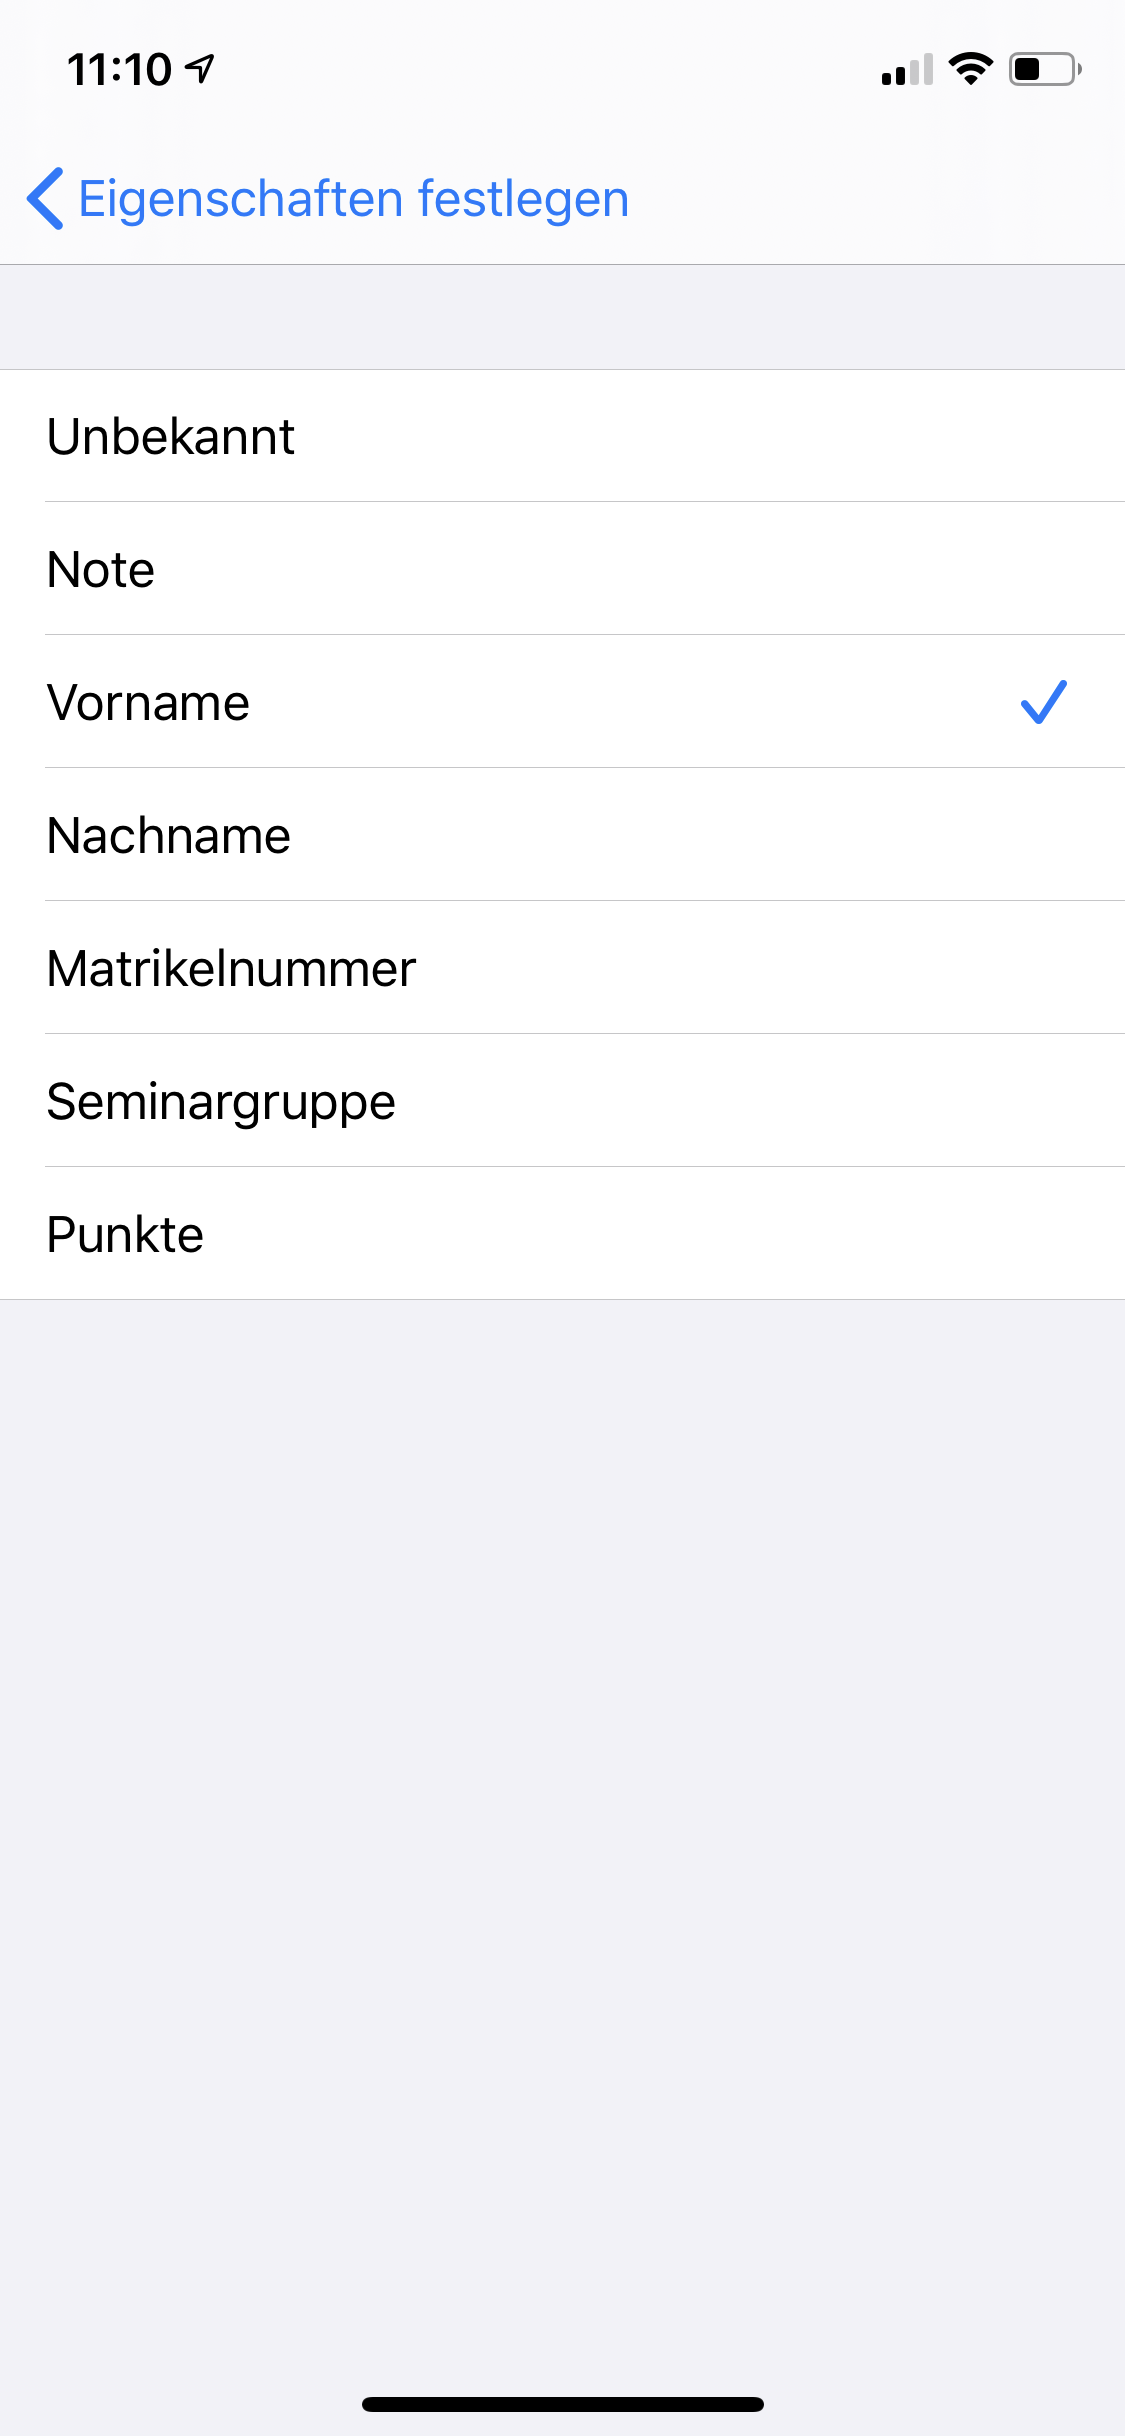
\includegraphics[width=0.96\textwidth]{img/V6}}
        				\caption{Auswahl des Datentyps}
        				\label{fig:v6}
    				\end{subfigure}
    				\begin{subfigure}[t]{0.3\textwidth}
       					\frame{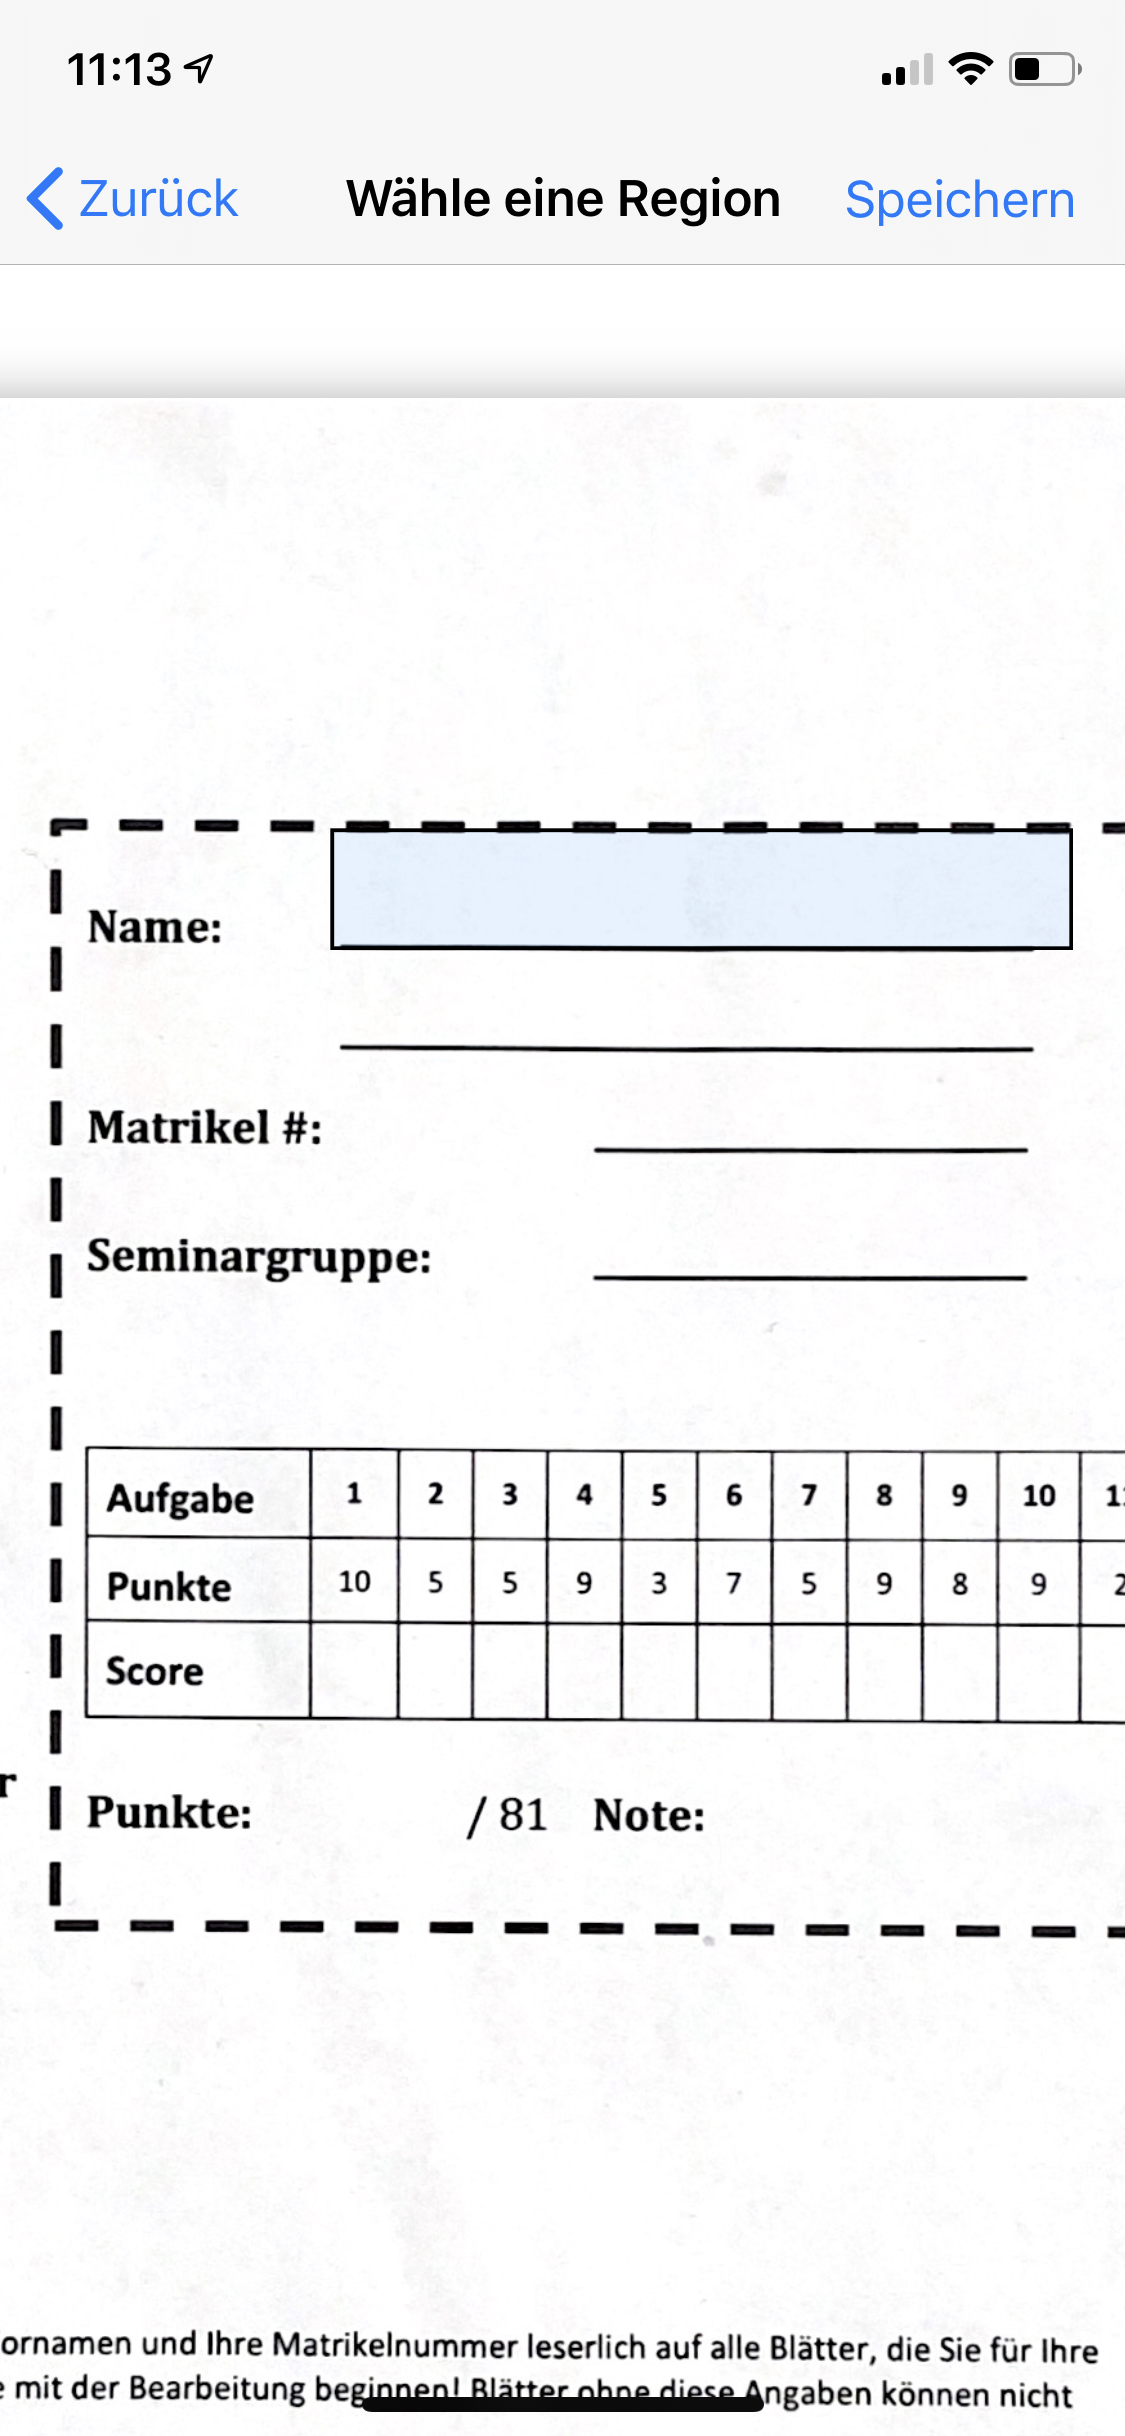
\includegraphics[width=0.96\textwidth]{img/V7}}
        				\caption{Markierung der Region auf dem Dokument}
        				\label{fig:v7}
    				\end{subfigure}
    				\caption{Views zur Erstellung von Regionen}
    				\label{fig:erstellung2}
				\end{figure}
			
			\vspace{-5mm}
			\subsubsection*{Kontrollmechanismen erstellen}
				Schließlich können die Kontrollmechanismen erstellt werden. Diese Funktion ist allerdings noch nicht sehr weit fortgeschritten und beinhaltet aktuell nur den Kontrollmechanismen-Typ zum Vergleichen von Regionen, wie im \autoref{ch:konzept} beschrieben ist. Beim Erstellen einer Kontrolle dieses Typs müssen zwei Regionen aus gewählt werden (siehe \autoref{fig:l2}), deren Inhalt nach der Texterkennung auf Gleichheit überprüft wird. Bei der Wahl der zwei Regionen stehen alle vorher angelegten Regionen, wie in \autoref{fig:l3} zu sehen ist, zur Verfügung. In \autoref{fig:l1} sind die bereits angelegten Kontrollmechanismen dieser Scan-Vorlage zu sehen sowie ein Button zum Speichern der Vorlage.
				
				\begin{figure}[h!]
    				\centering
					\begin{subfigure}[t]{0.3\textwidth}
       					\frame{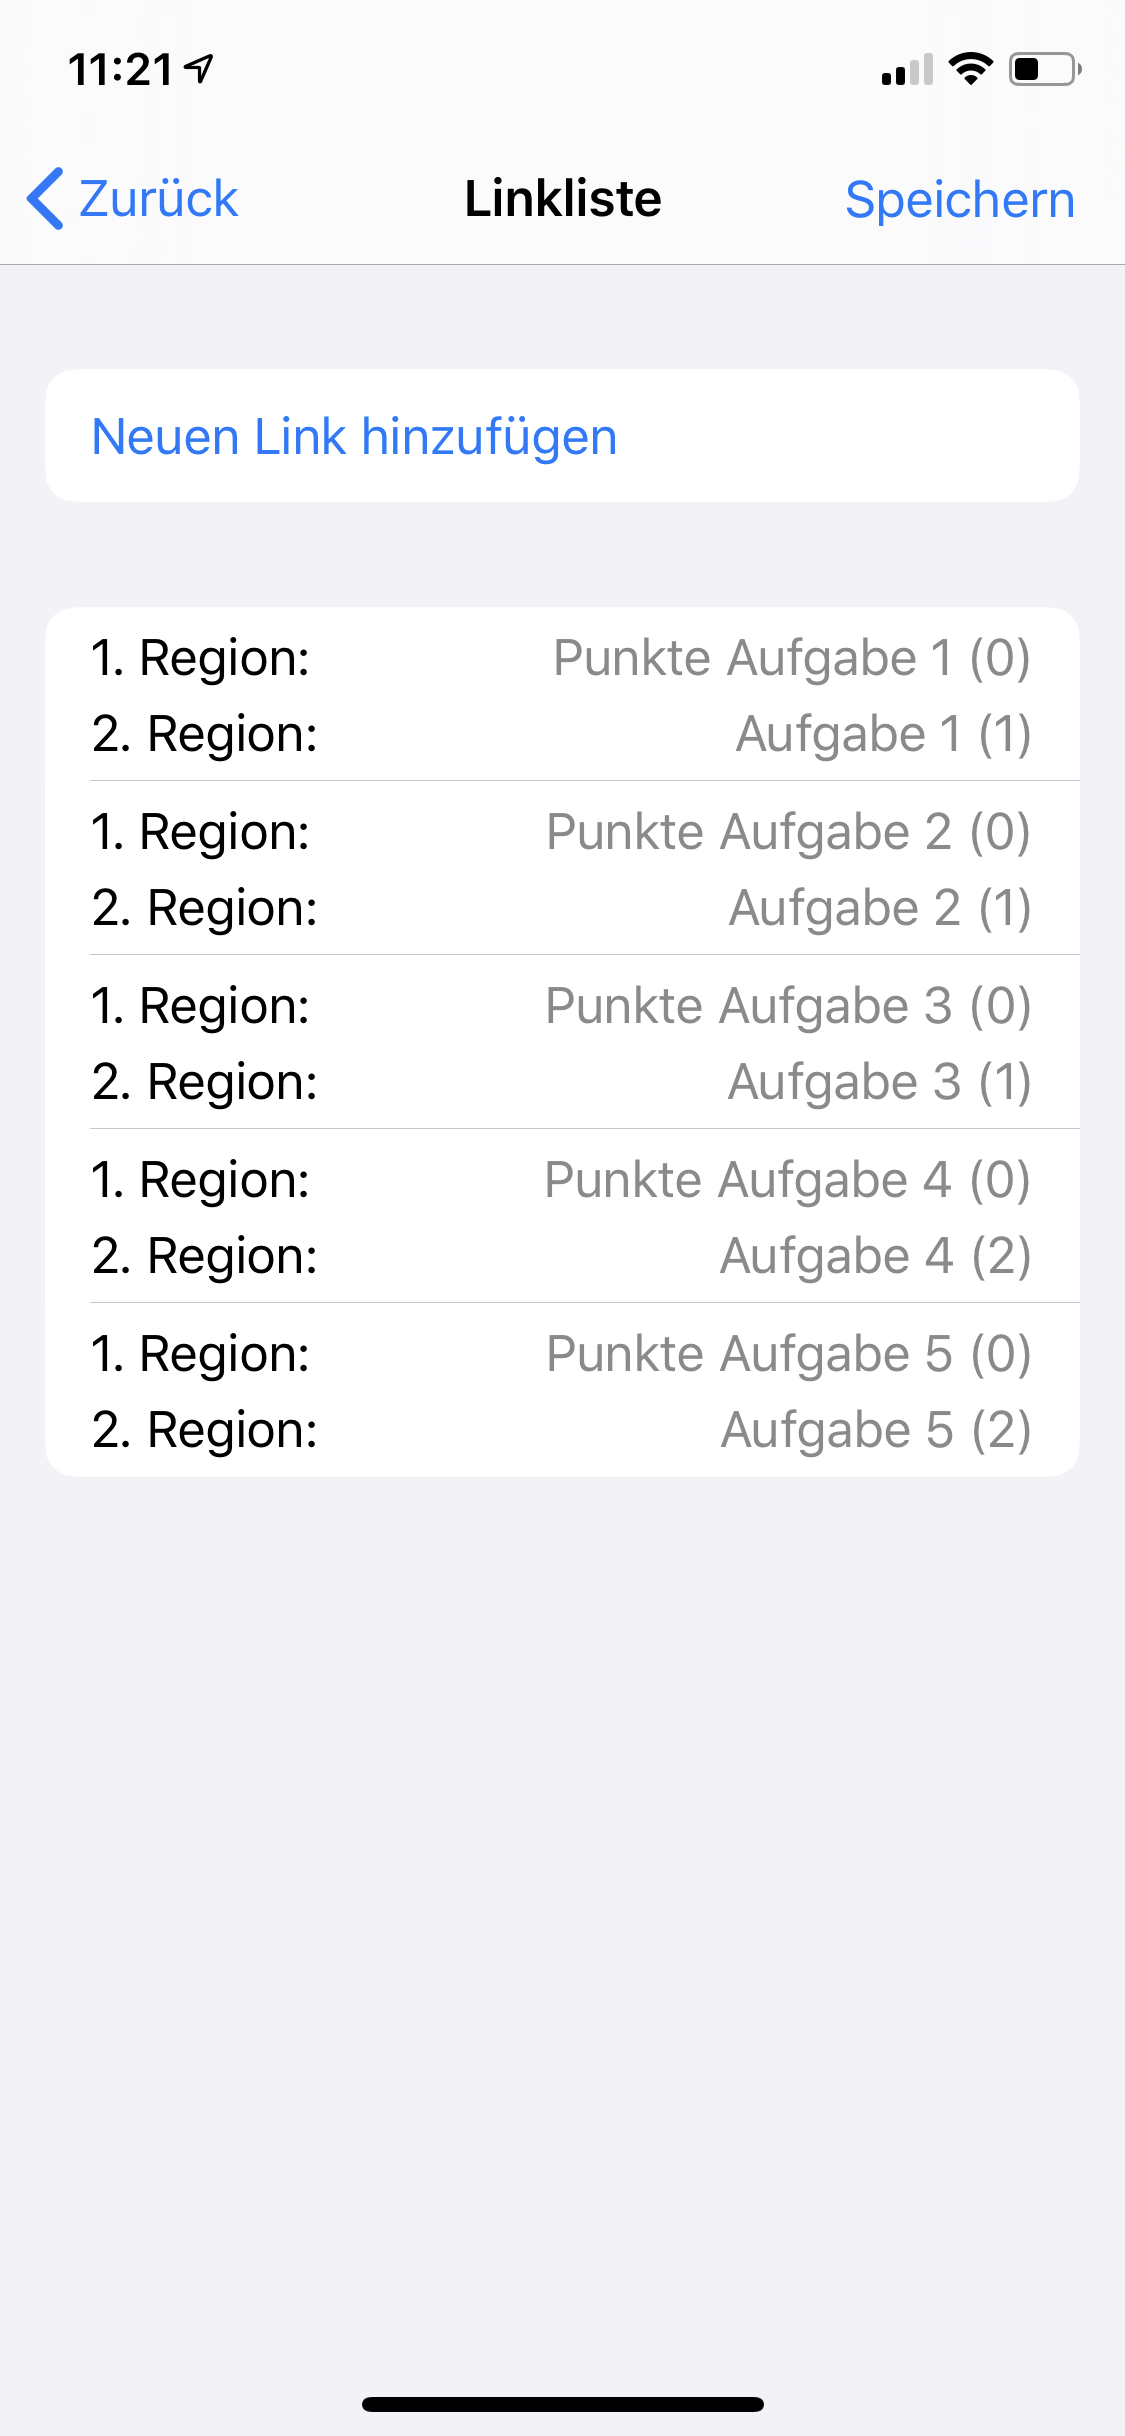
\includegraphics[width=0.96\textwidth]{img/L6}}
        				\caption{Kontroll-Liste mit angelegten Kontrollmechanismen}
        				\label{fig:l1}
    				\end{subfigure}
    				\begin{subfigure}[t]{0.3\textwidth}
       					\frame{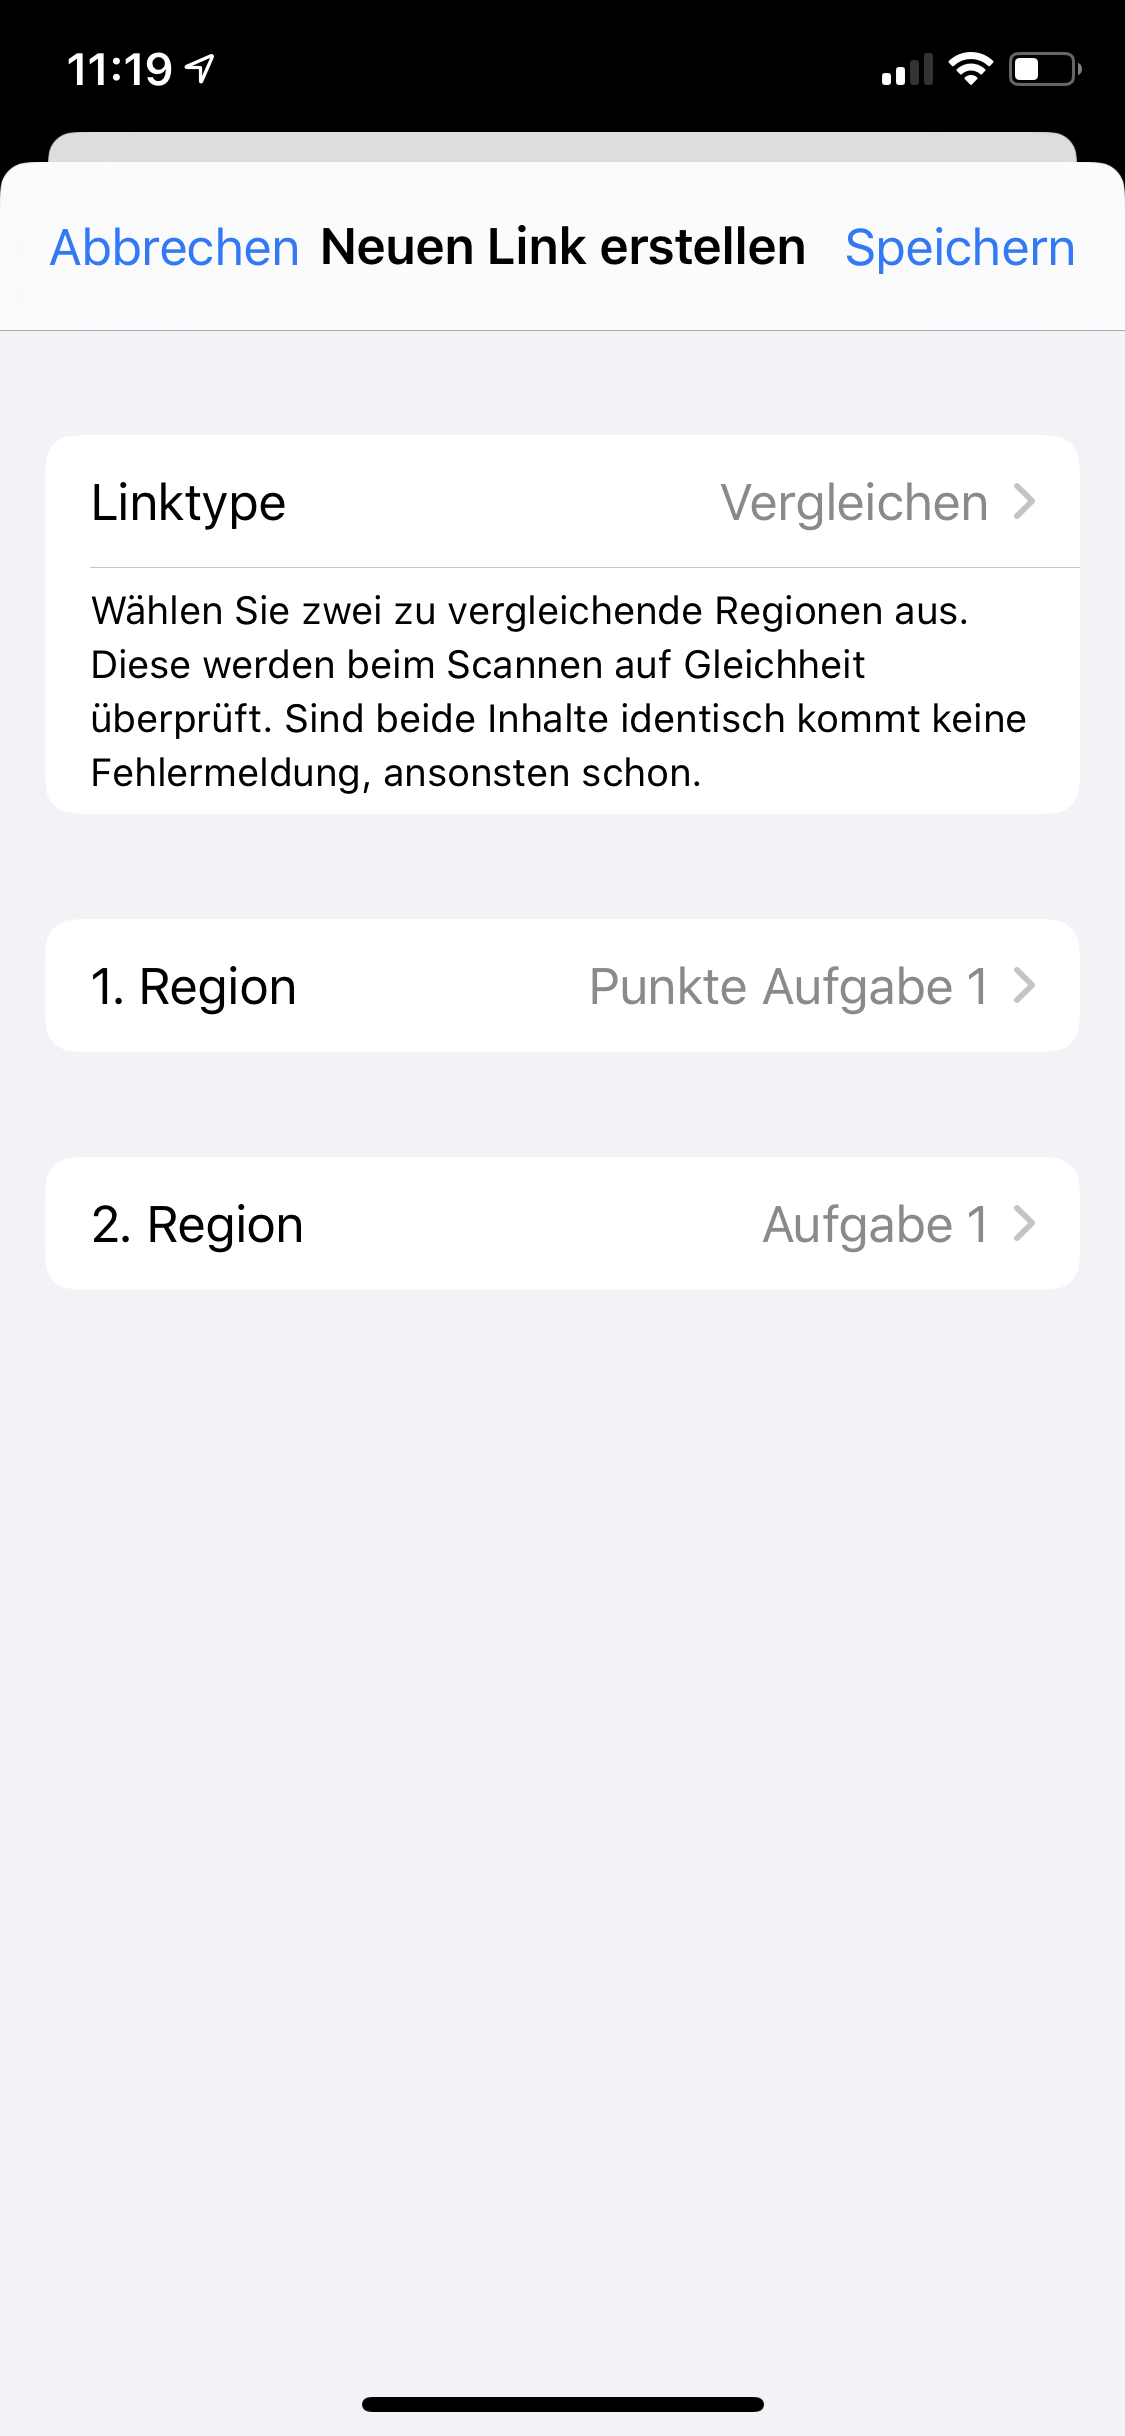
\includegraphics[width=0.96\textwidth]{img/L4}}
        				\caption{View zur Erstellung einer Kontrolle}
        				\label{fig:l2}
    				\end{subfigure}
    				\begin{subfigure}[t]{0.3\textwidth}
       					\frame{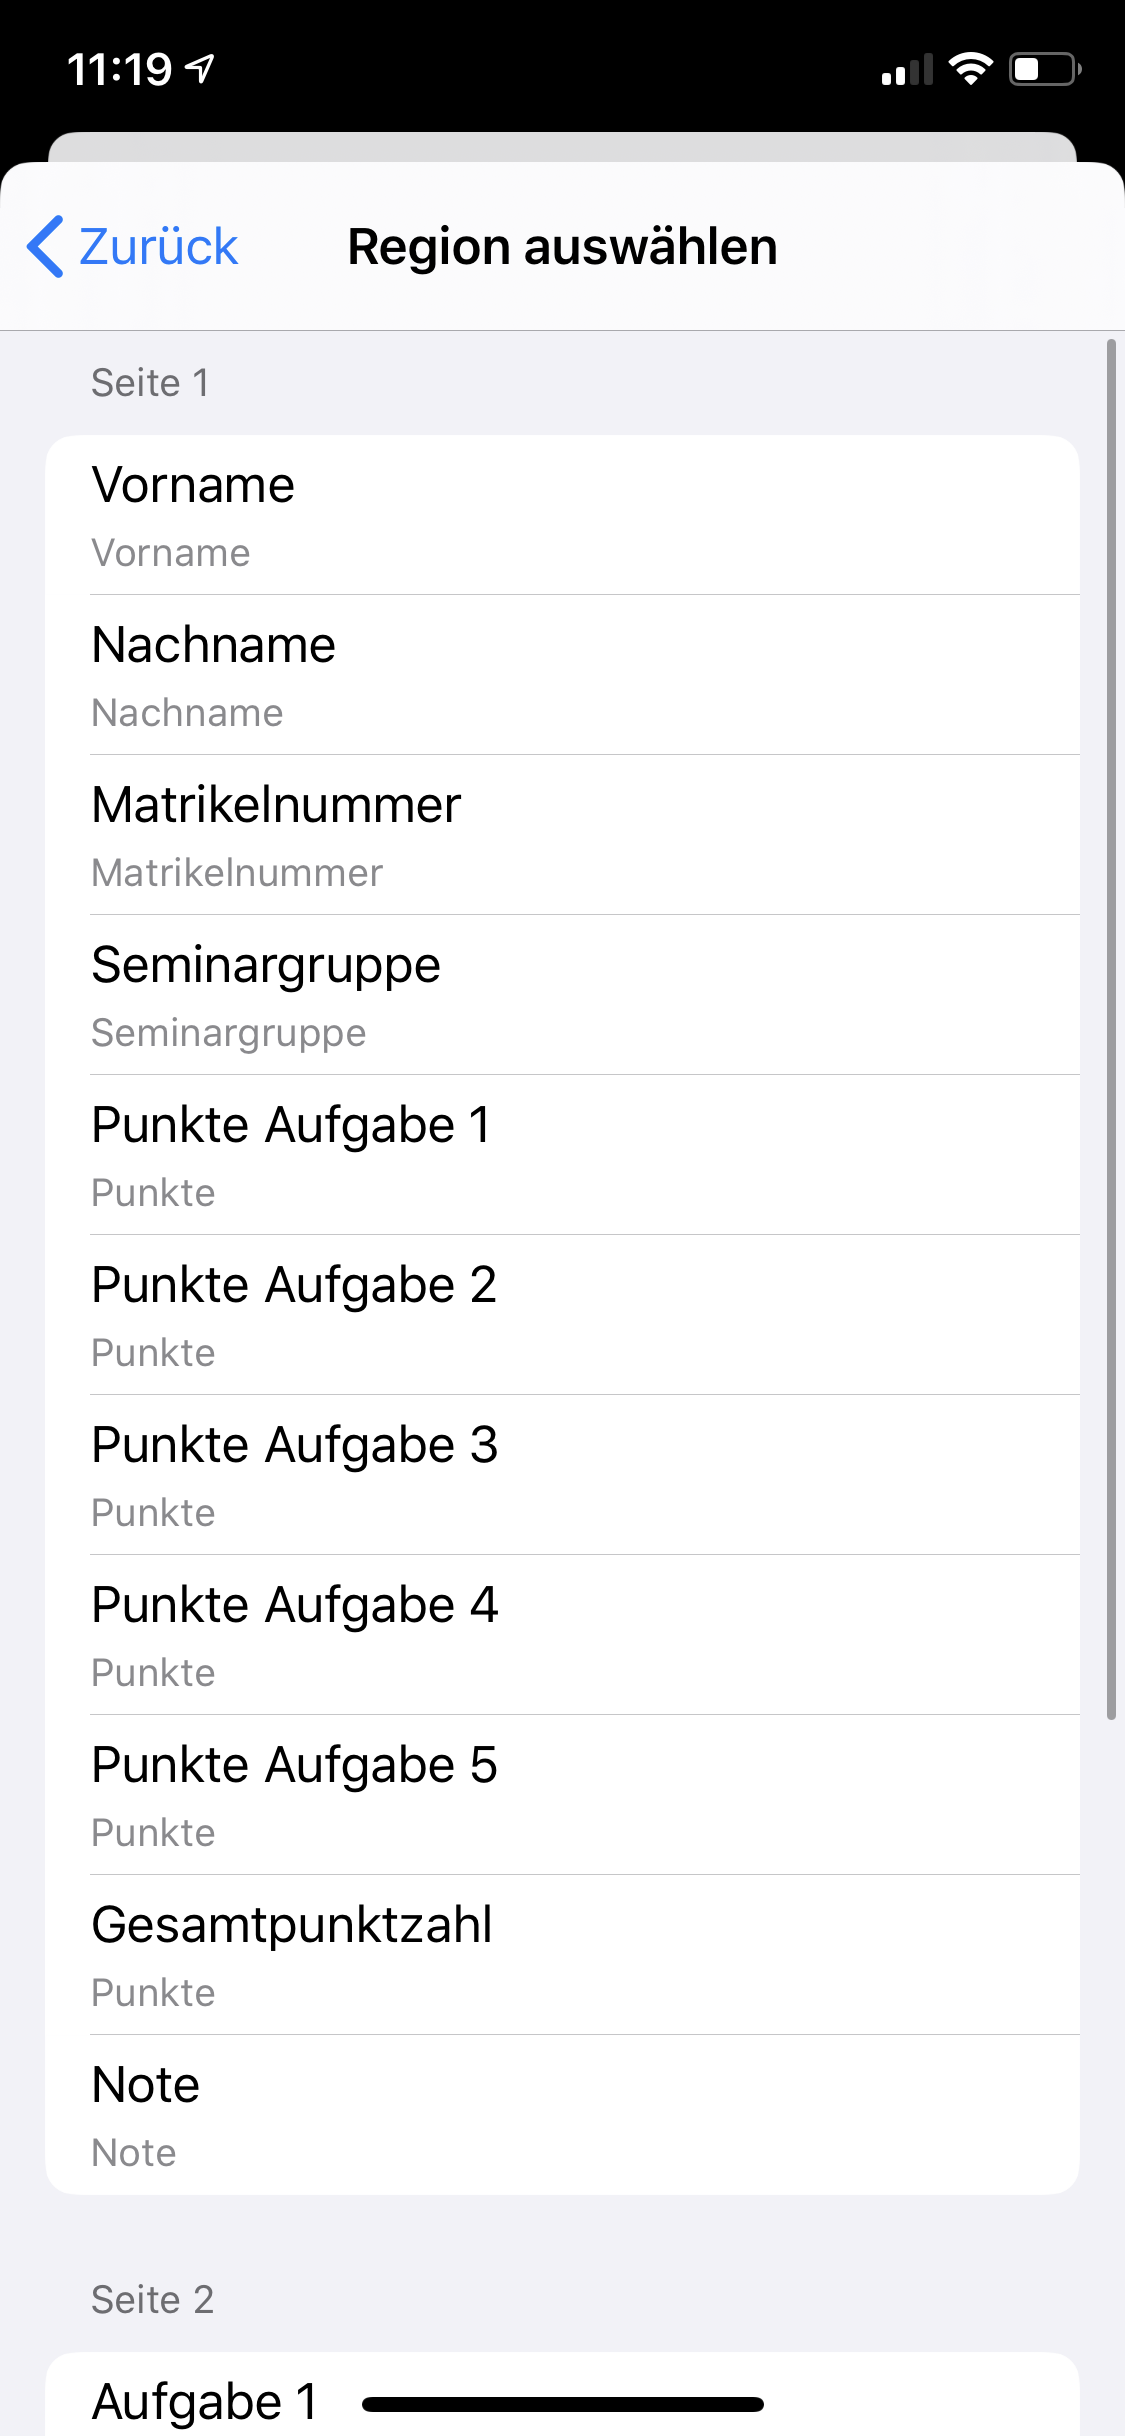
\includegraphics[width=0.96\textwidth]{img/L3}}
        				\caption{View zur Auswahl einer Region}
        				\label{fig:l3}
    				\end{subfigure}
    				\caption{Views zur Erstellung von Kontrollmechanismen}
					\label{fig:link1}
				\end{figure}

			\subsubsection*{Scan-Vorlage speichern}
				Die Speicherung erfolgt in mehreren Schritten. Dazu werden die entsprechenden Server-Schnittstellen in einer bestimmten Reihenfolge aufgerufen. Für genauere Details zur API des Servers siehe im Praktikumsbericht von Tobias Kallauke.
				
				%%%%%%%%%%%%%%%%%%%%%%
	%			... und wie die Vorlage versendet wird ...
				%%%%%%%%%%%%%%%%%%%%%%
			
%				Im folgenden Abschnitt, ist beschrieben, in welcher Reihenfolge das Hochladen einer Vorlage zum Server geschieht. Dabei werden mögliche Fehler von Seiten des Server, der Internetverbindung und des Clients ignoriert. Jedoch ist im aktuellen Stand der App das Abfangen des Fehler schon integriert, eventuelle Fehlerbehandlung aber nicht.
%				\begin{enumerate}
%					\item Der Name und die Beschreibung der Vorlage sowie die Liste an Kontrollmechanismen wird gesendet. In der Antwort des Servers befindet sich  die Vorlagen-ID\nomenclature{ID}{Steht für einen einzigartigen Identifikator} , die in den nächsten Schritten benötigt wird. 
%					\item Die Bilder der Seiten werden gesendet. Als Antwort zu jedem Bild wird der Pfad zurück geschickt, wo das Bild vom Server gespeichert wurde. Dieser Pfad wird im nächsten Schritt benötigt.
%					\item Die Seiten mit einer Seiten-Nummer und dem Pfad zu dem Bild, wird mit der Vorlagen-ID gesendet. Als Antwort wird eine Seiten-ID zurückgegeben, die im nächsten Schritt verwendet wird.
%					\item Die Regionen der Seiten werden gesendet. Eine Region hat X- und Y-Koordinaten. Diese repräsentieren den Abstand vom Bildursprung, der sich in jedem Bild oben links befindet. Außerdem besitzt eine Region noch eine Höhe und Breite sowie einen Namen und einen Datentyp (\ref{fig:v5} und \ref{fig:v7}). Die Koordinaten sowie die Höhe und Breite sind alle in Pixel angegeben. Zusammen mit der Seiten-ID wird das Attribute an den Server gesendet.
%				\end{enumerate}
			
		\newpage
		\subsection{Scan-Vorlage verwenden}
			Bei der Implementierung dieses Arbeitsschrittes wurde das Flussdiagramm \ref{fig:verwenden_flow}, welches im \autoref{ch:workflow} zu finden ist, benutzt.
			
			Um eine Klausur zu digitalisieren, muss die vorher erstellte Scan-Vorlage ausgewählt werden (\ref{fig:liste1}). Danach ist das Einscannen einer Klausur über einen Button möglich (\ref{fig:liste2}). Bevor die Bilder aufgenommen werden können, erscheint ein Dialogfenster (\ref{fig:liste3}). Der Benutzer muss entscheiden, welche OCR-Engine benutzt werden soll. Aktuell gibt es zwei Möglichkeiten:
			\vspace{-5mm}
			\begin{itemize}
				\item Die OCR-Engine des Vision-Frameworks, welche direkt auf dem Gerät und ohne eine Internetverbindung die Texterkennung durchführt,  
				\item oder die OCR-Engine Tesseract, die über eine Schnittstelle des Servers aufzurufen ist.
			\end{itemize}

				
			\begin{figure}[h!]
    			\centering
				\begin{subfigure}[t]{0.3\textwidth}
       				\frame{
\includegraphics[width=0.96\textwidth]{img/liste1}}
        			\caption{Übersicht aller Scan-Vorlagen}
        			\label{fig:liste1}
    			\end{subfigure}
    			\begin{subfigure}[t]{0.3\textwidth}
       				\frame{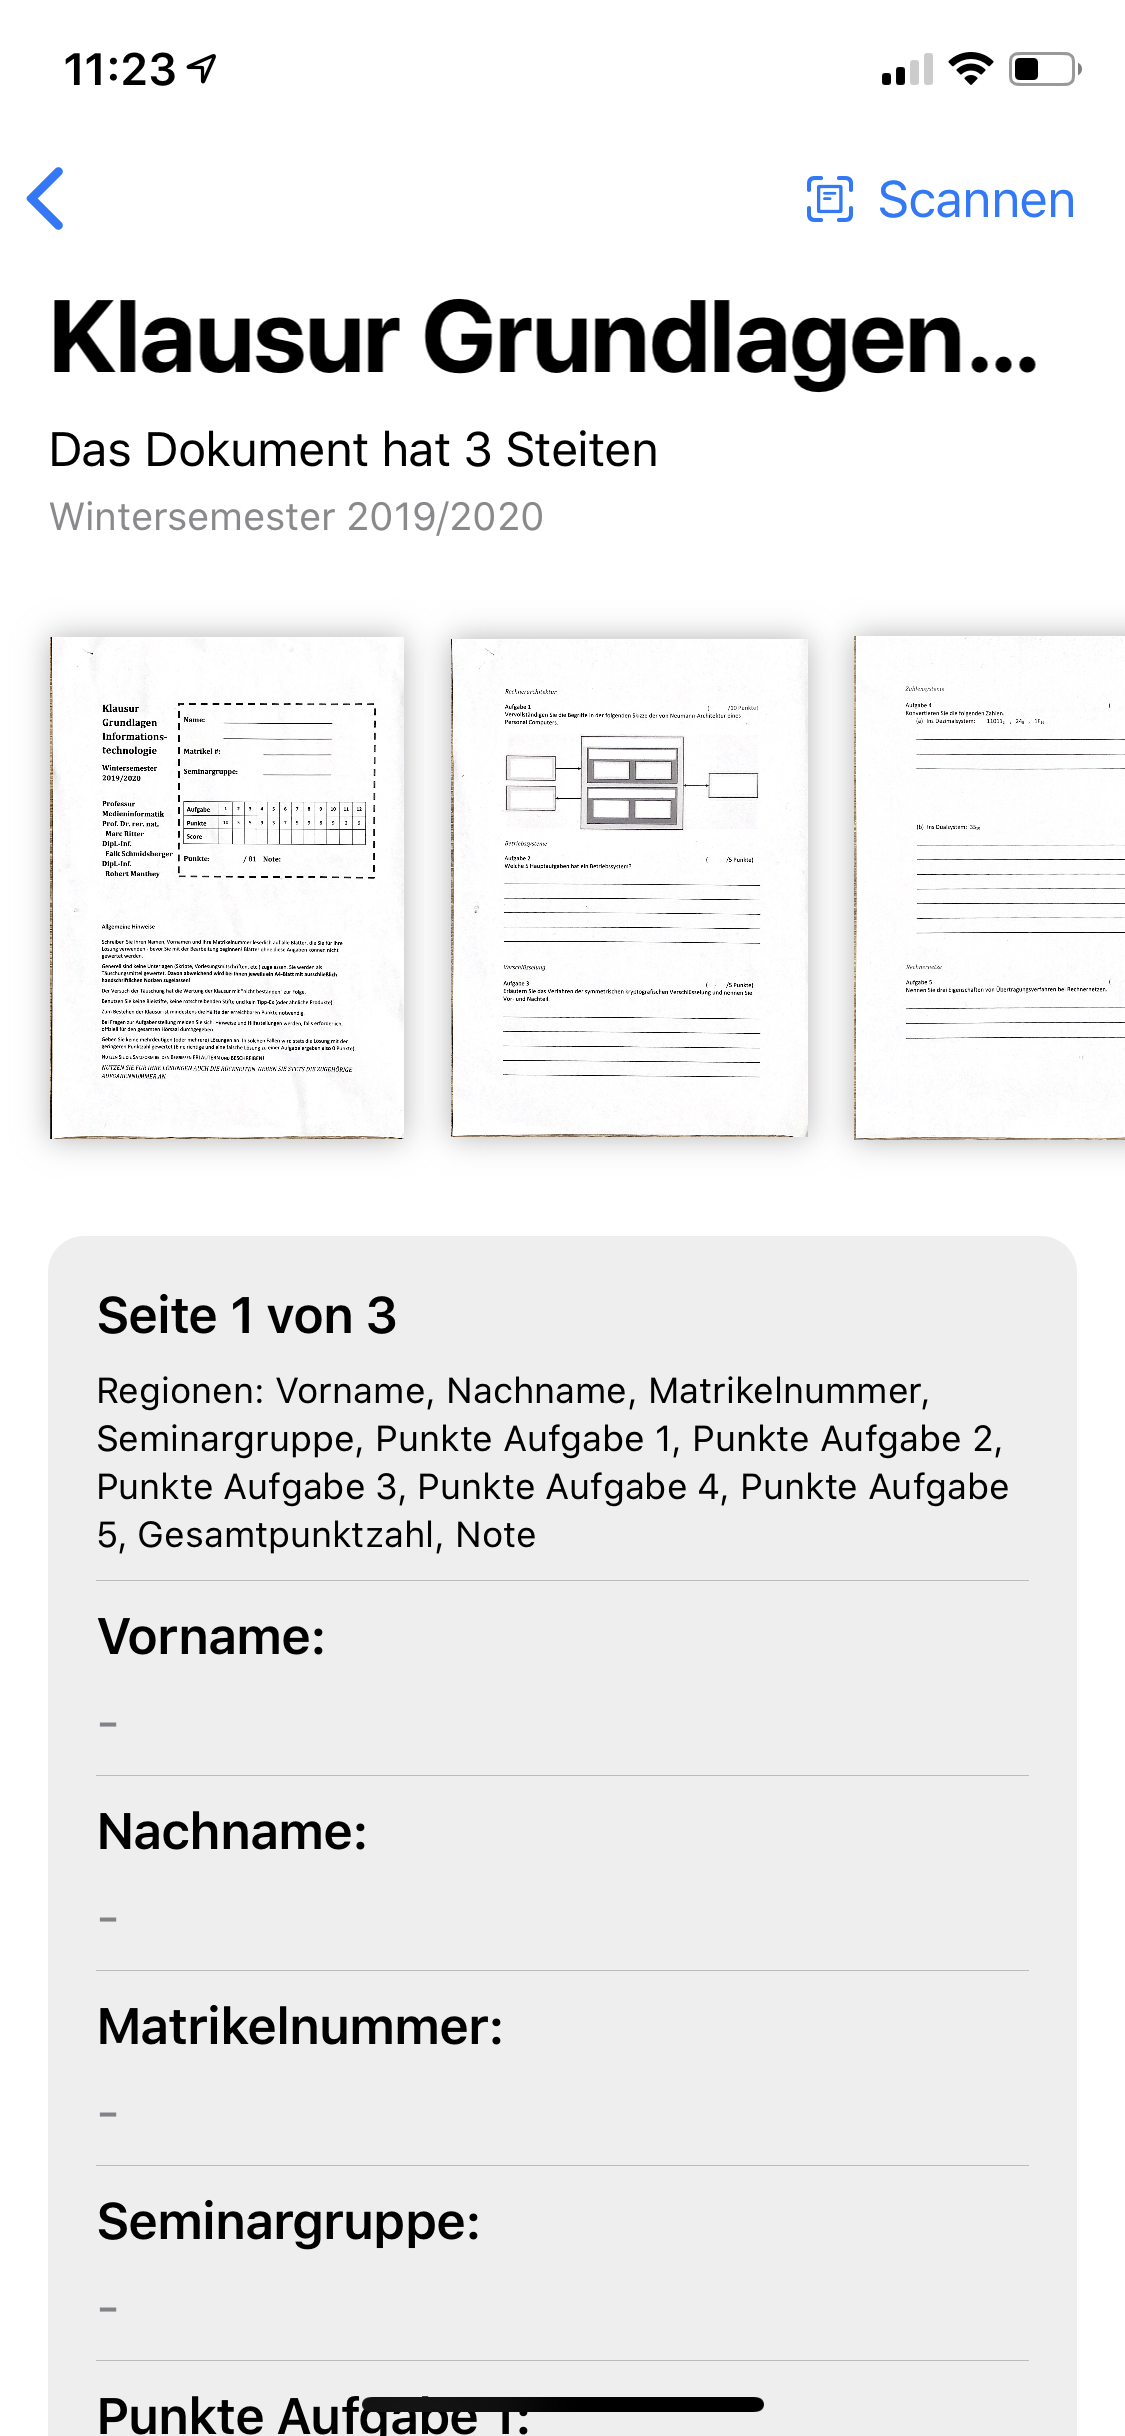
\includegraphics[width=0.96\textwidth]{img/liste2}}
        			\caption{Detailansicht einer Scan-Vorlage}
        			\label{fig:liste2}
    			\end{subfigure}
    			\begin{subfigure}[t]{0.3\textwidth}
       				\frame{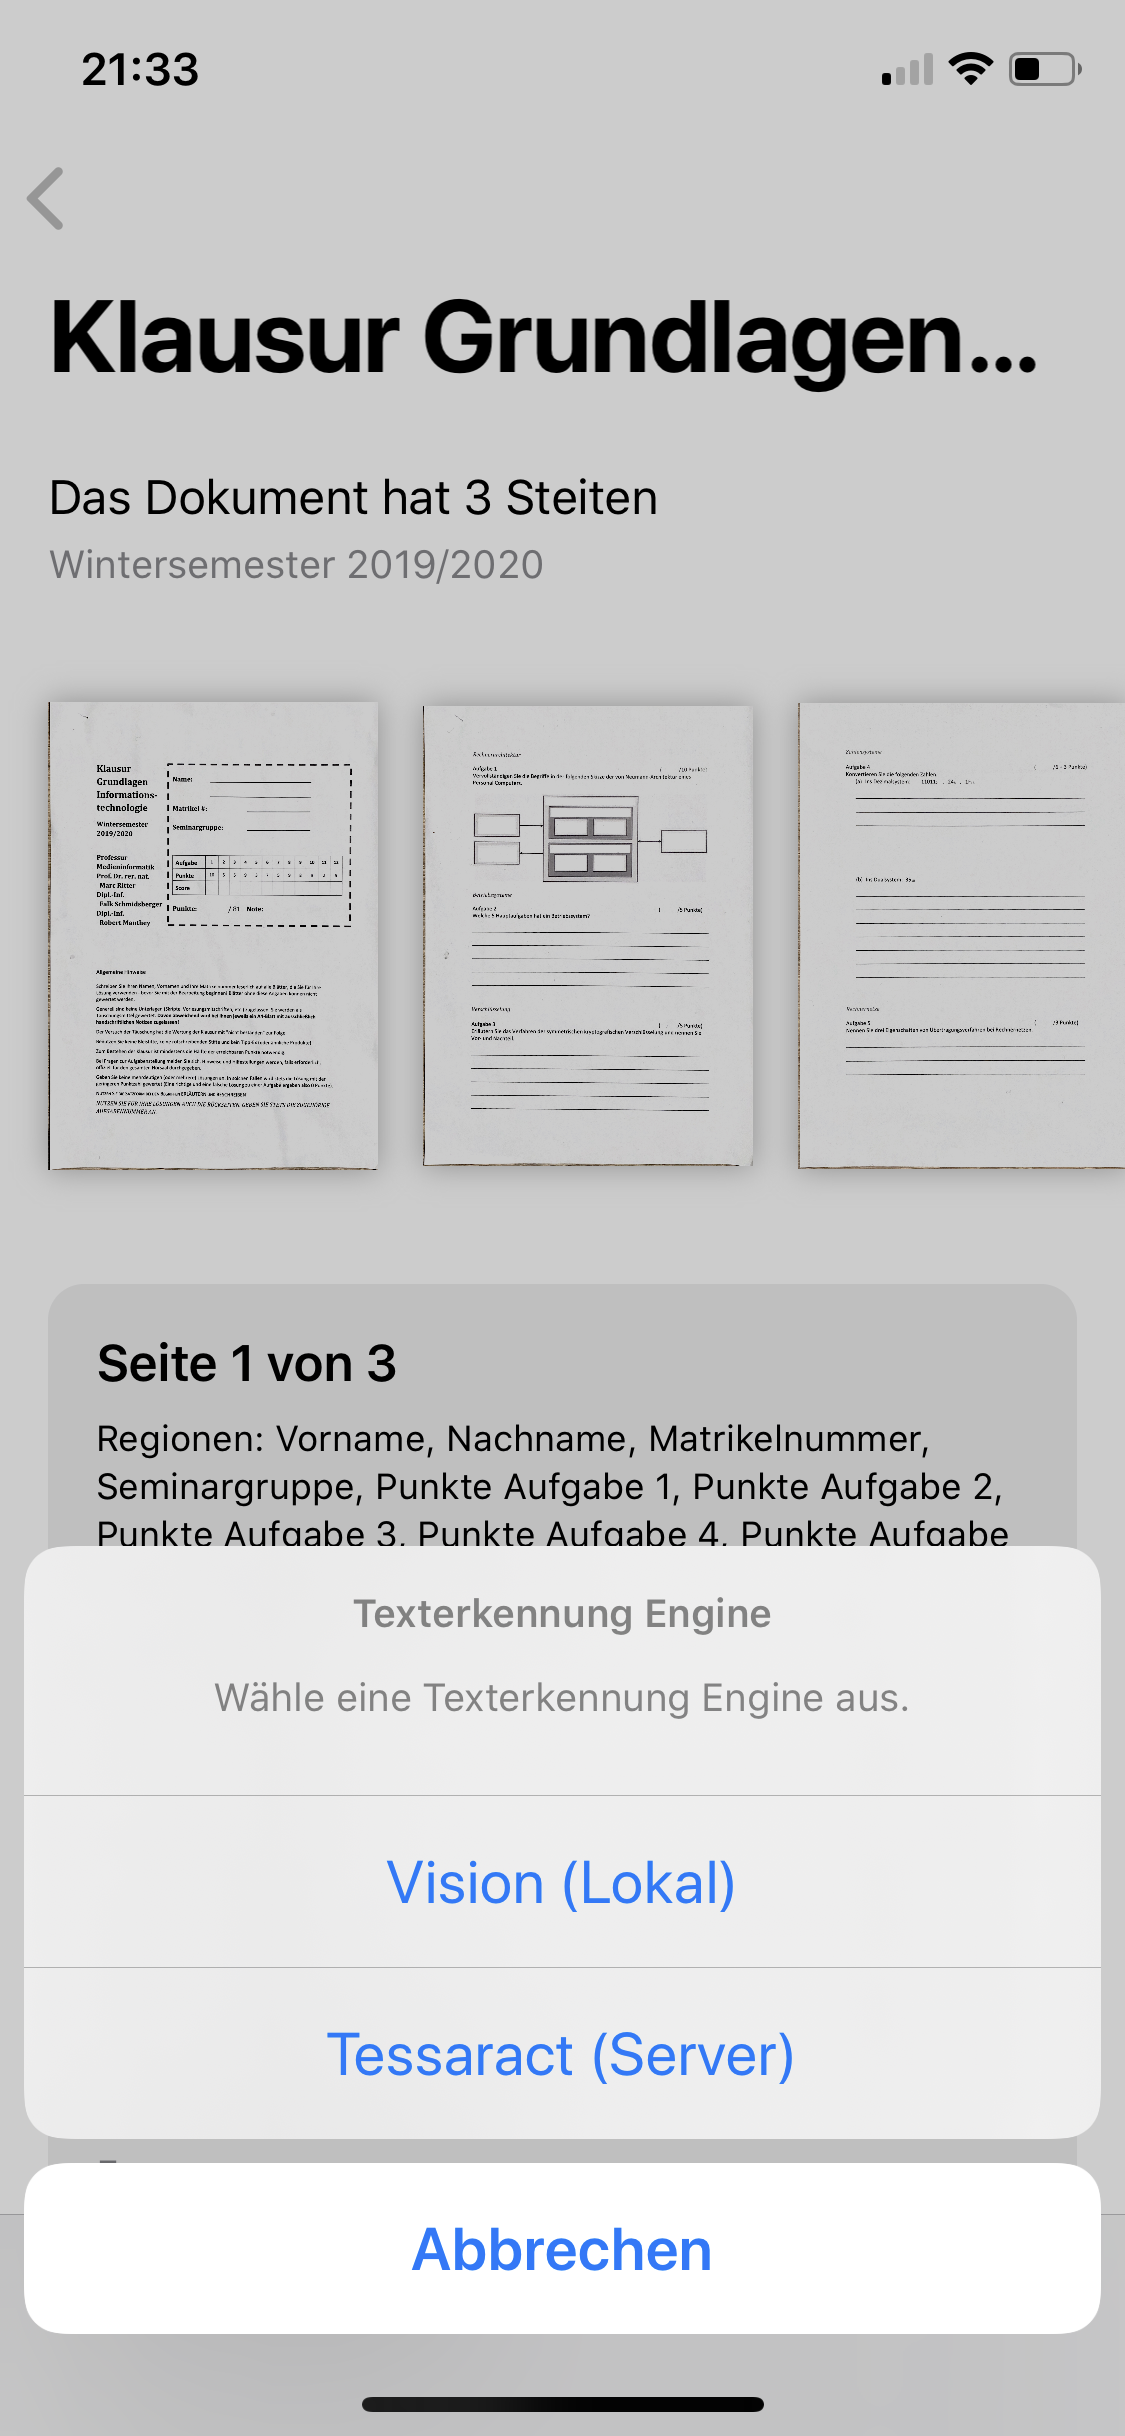
\includegraphics[width=0.96\textwidth]{img/ocr1}}
        			\caption{Liste der Kontroll-Mechanismen}
        			\label{fig:liste3}
    			\end{subfigure}
    			\caption{Dialogfenster zur Auswahl der OCR-Engine}
				\label{fig:vorlagen}
			\end{figure}
			
			Nun erscheint die Scan-View und die Bilder können aufgenommen werden. Wichtig dabei ist, dass die Seiten beim Fotografieren dieselbe Reihenfolge, wie in der Scan-Vorlage haben. Auch muss die Anzahl der eingescannten Seiten mit denen in der Vorlage übereinstimmen. Mithilfe der Scan-View wird die Seite aus dem Bild ausgeschnitten, geglättet und der Kontrast des Bildes so verändert, dass Schriftzeichen leichter zu erkennen sind und Schatten bzw. Falten verschwinden.
			
			Nach dem Einscannen der Klausurseiten beginnt der Prozess der Texterkennung. Durch Aktivitätsanzeigen wird dem Benutzer mitgeteilt, dass die Anwendung gerade arbeitet. Die Abläufe der online OCR-Engine und des Vision Frameworks unterscheiden sich deutlich.	

			\subsubsection*{Ablauf mit Vision}
				Bei der Verwendung von Vision gibt es folgende grobe Schritte:
				\vspace{-5mm}
				\begin{enumerate}
					\item Die markierten Regionen werden in der Vorlage auf die neuen Fotos angewendet.
					\item Mithilfe der Regionen werden Bildausschnitte aus den Fotos erstellt.
					\item Die Ausschnitte werden in die ausgewählte OCR-Engine überführt.
					\item Darstellung der Texterkennungsergebnisse auf der View.
				\end{enumerate}
					
				\paragraph*{Zu 1.: Die markierten Regionen werden in der Vorlage auf die neuen Fotos angewendet.}
					Nun wird jedes Foto des neuen Scans mit den Regionen der jeweiligen Seite der Scan-Vorlage verarbeitet. 
					Wie in den Abbildungen \ref{fig:seite1} und \ref{fig:seite2} zu sehen ist, haben beide, durch die App entstandenen Bilder, unterschiedliche Maße. Die \autoref{fig:seite1} ist größer und etwas breiter als die \autoref{fig:seite2}. Das liegt daran, dass sich der Winkel und der Abstand der Kamera zum Dokument zwischen den Aufnahmen geändert hat. Wenn die Bilder in der Vorlage nicht genau so groß sind, wie die Bilder des neuen Scans, können wichtige Informationen durch die absoluten Positionen der Regionen abgeschnitten werden. Aus diesem Grund müssen nun die absoluten in relative Positionen umgerechnet werden. Gleiches gilt für die Höhe und Breite der Regionen.

				\paragraph*{Zu 2.: Mithilfe der Regionen werden Bildausschnitte aus den Fotos erstellen.}
					Nachdem die neue Position und die Maße berechnet wurden, entstehen daraus Bildausschnitte für die Texterkennung. Bei falscher Erstellung der Vorlagen oder bei falschem Einscannen der Klausur kann es trotzdem passieren, dass Teile der Regionen wegfallen. Dazu im \autoref{ssc:erkennen} mehr.
				
				\paragraph*{Zu 3.: Die Ausschnitte werden in die ausgewählte OCR-Engine überführt.}
					Zu jedem Bildausschnitt wird eine sogenannte Texterkennungsanfrage konfiguriert. Hierfür wird weiterhin die zugehörige Region benötigt. In der Konfiguration werden an Hand des Region-Datentyps (\ref{fig:v6}) unterschiedliche Einstellungen getroffen. Beispielsweise wird beim Datentyp Note eine sogenannte costum words-Liste verwendet. Sie beinhaltet alle zu erwartende Ergebnisse bzw. Noten. Die Liste hat in der Worterkennungsphase Vorrang vor dem Standard-Wörterbuch, wie schon im \autoref{ch:konzept} erwähnt und sorgt für bessere Ergebnisse\footurl{Vision \textit{costumWords} Dokumentation}{https://developer.apple.com/documentation/vision/vnrecognizetextrequest/3152640-customwords}.						
					Standardmäßig werden bei der Bearbeitung einer Texterkennungsanfrage zunächst alle Zeichen im Eingabebild lokalisiert und dann jede Zeichenfolge analysiert\footurl{Quelle: \textit{VNRecognizeTextRequest} Dokumentation}{https://developer.apple.com/documentation/vision/vnrecognizetextrequest}. Anschließend wird eine Korrektur der erkannten Wörter auf der Grundlage eines Wörterbuchs und anderer Wahrscheinlichkeitsheuristiken für Zeichenpaare durchgeführt \cite{apple_text_2019}. Der genaue Ablauf der Texterkennung bzw. die verwendeten Algorithmen von Vision sind allerdings nicht bekannt. 
				
					Nach der Texterkennung durch Vision erfolgt in einigen Fällen noch eine selbst entwickelte Korrektur, wie sie in \autoref{ch:konzept} \autoref{sc:erweiterungkonzept} beschrieben ist. Wieder ist der Regionen-Datentyp (\ref{fig:v6}) ausschlaggebend. Beispielsweise wird der Text einer vermeintlichen Seminargruppe mit allen in der App hinterlegten Seminargruppen verglichen. Das erkannte Wort wird durch den Seminargruppennamen mit der größten Übereinstimmung ersetzt und die confidence gegebenenfalls angepasst.
				
					Zuletzt werden die erkennten Texte bzw. Worte und deren confidence an den State-Container der App gesendet. Für die Ergebnisse der Texterkennung ist ein eigener State vorgesehen, in dem auch die Serverergebnisse von Tesseract gesichert werden. Somit ist das Anzeigen der Ergebnisse bei beiden OCR-Engines gleich.  
				
				\paragraph*{Zu 4.: Darstellung der Texterkennungsergebnisse auf der View.}
					Die Ergebnisse der Texterkennung und die jeweilige confidence werden auf der Benutzeroberfläche, nach Seiten sortiert, angezeigt (\ref{fig:ocr2}). Alle OCR-Ergebnisse können zudem noch angepasst werden. Abhängig vom Datentyp der Region passt sich die Tastatur beim Ändern der Texte an (\ref{fig:ocr3}). Beispielsweise sind die Tastaturen beim Anpassen von Noten und Punkten auf Zahlen und Dezimalpunkte spezialisiert. Zudem kann die confidence farblich (siehe \autoref{fig:ocr2}), aber auch als Zahlenwert (siehe \autoref{fig:ocr3}) angezeigt werden. Wurde kein Text erkannt, ist dementsprechend ein Warnsymbol an der Stelle der confidence zu sehen.  
 
 			\begin{figure}[h!]
    			\centering
    			\begin{subfigure}[t]{0.3\textwidth}
       				\frame{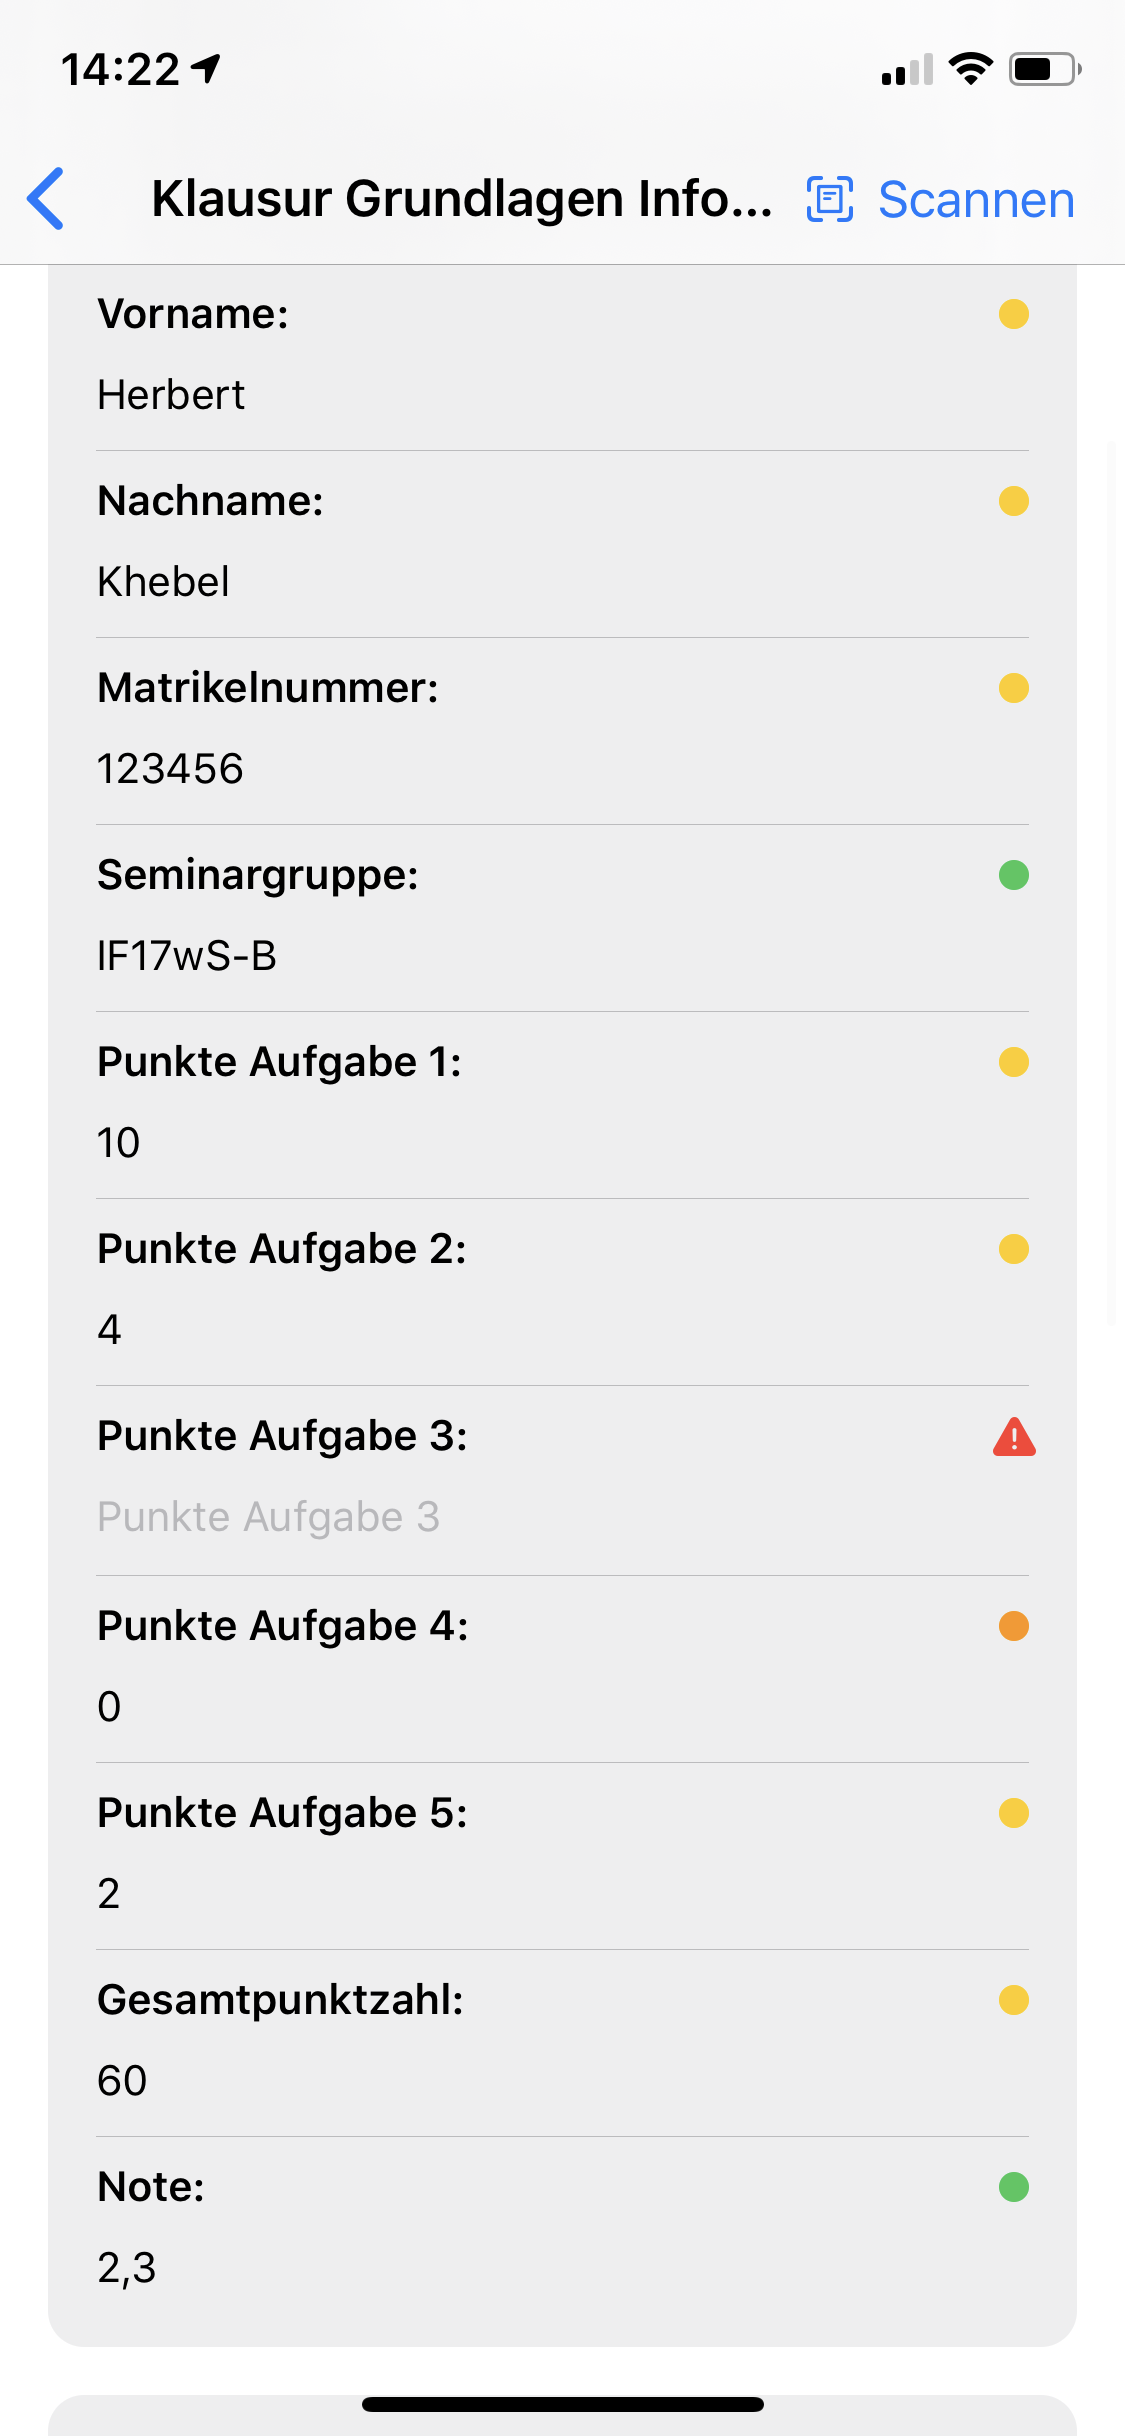
\includegraphics[width=0.96\textwidth]{img/ocr2}}
        			\caption{Übersicht nach der Texterkennung mit farblicher confidence}
        			\label{fig:ocr2}
    			\end{subfigure}
    			\begin{subfigure}[t]{0.3\textwidth}
       				\frame{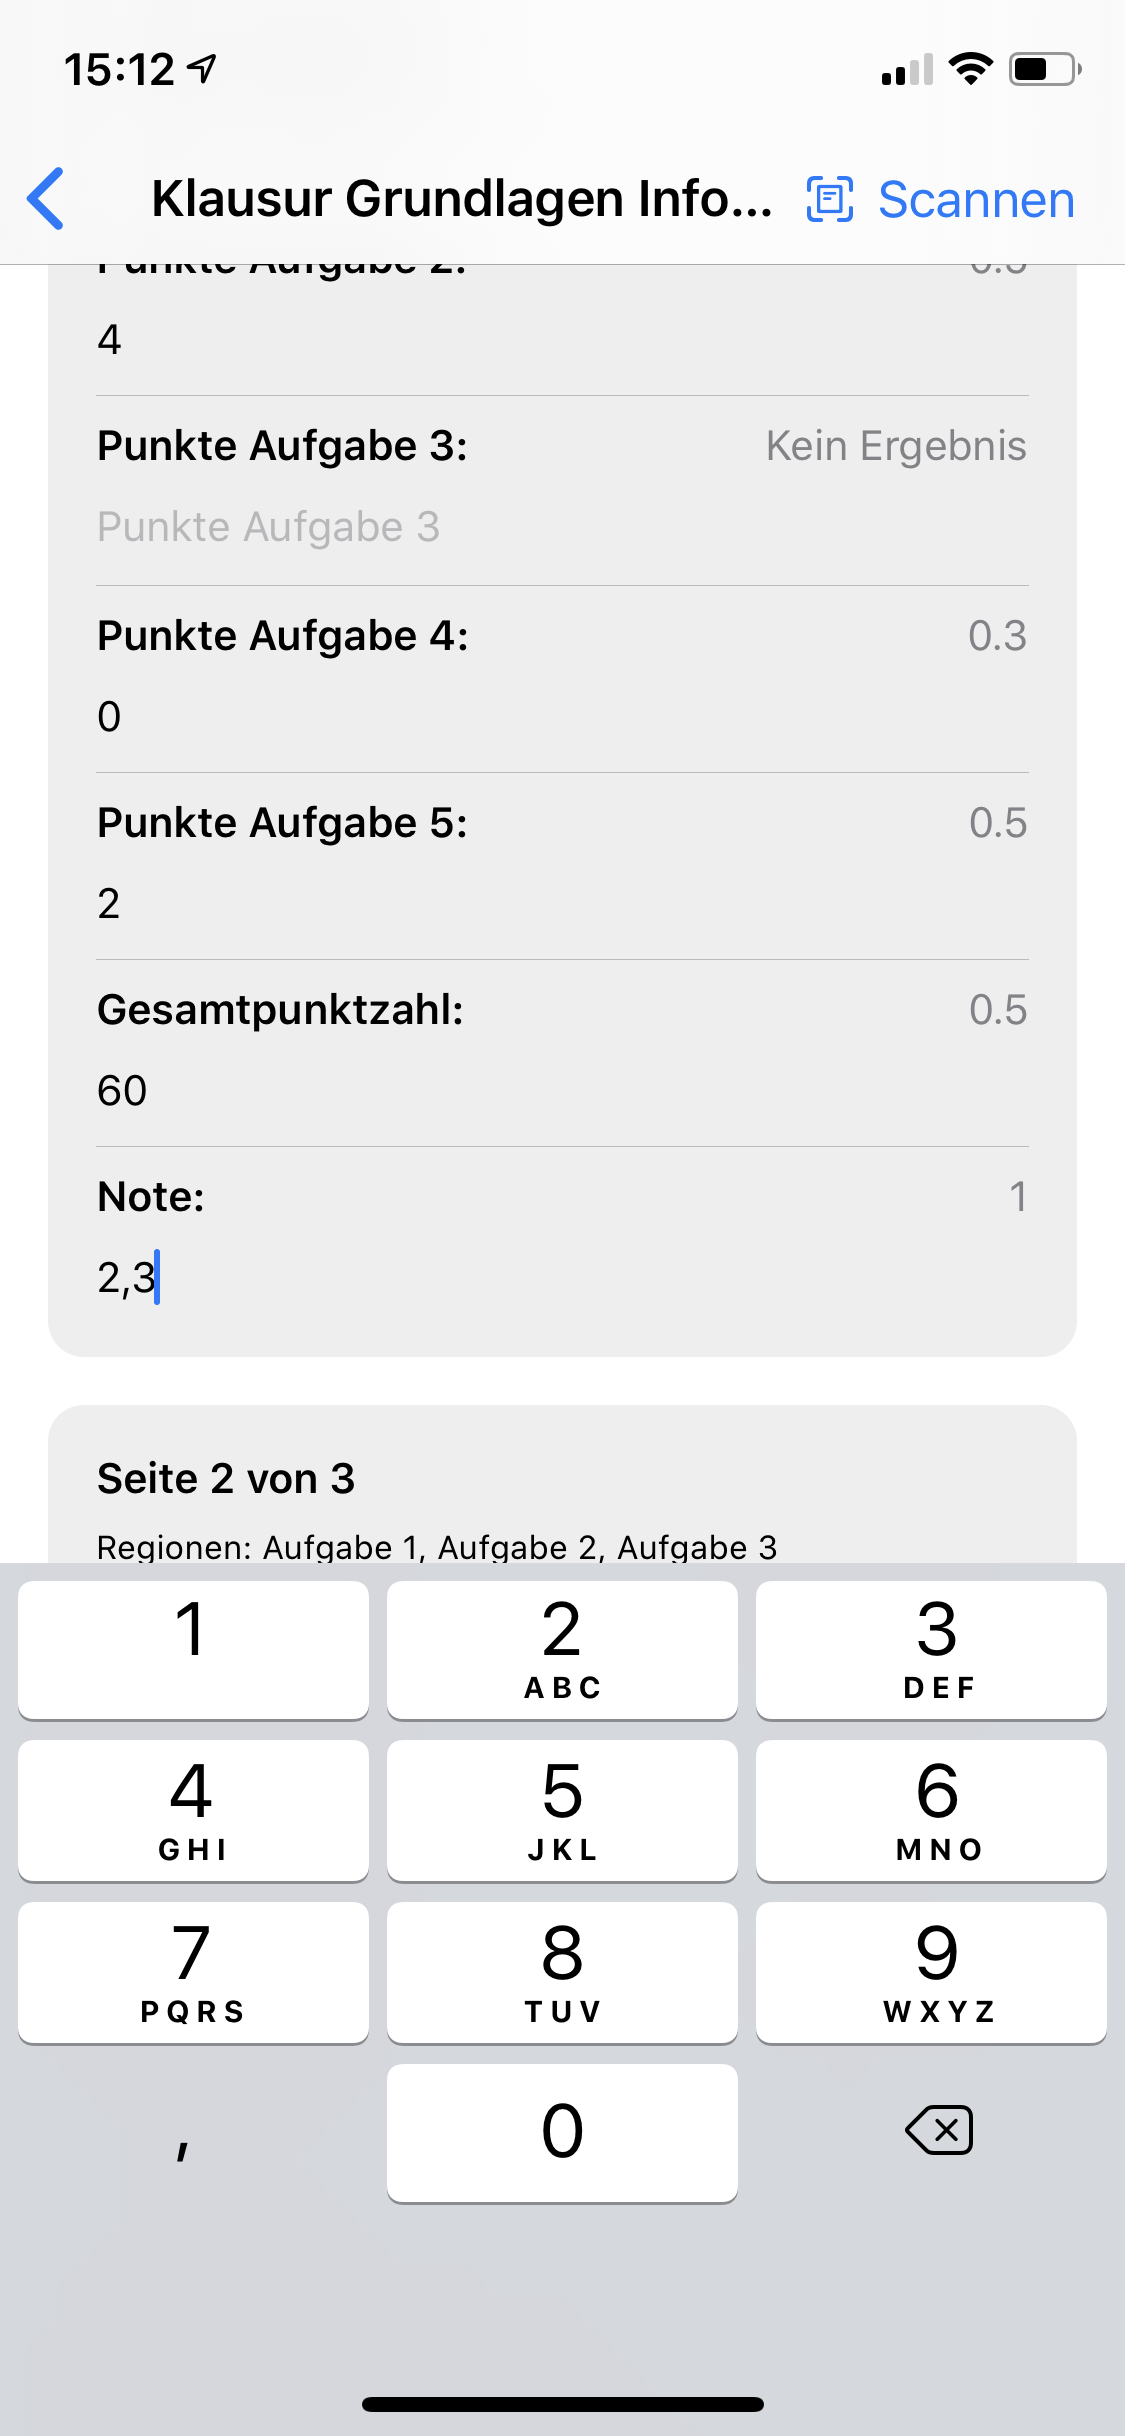
\includegraphics[width=0.96\textwidth]{img/ocr3}}
        			\caption{Änderung der Note mit spezieller Tastatur für Dezimalzahlen und confidence als Zahlenwert}
        			\label{fig:ocr3}
    			\end{subfigure}
    			\begin{subfigure}[t]{0.3\textwidth}
       				\frame{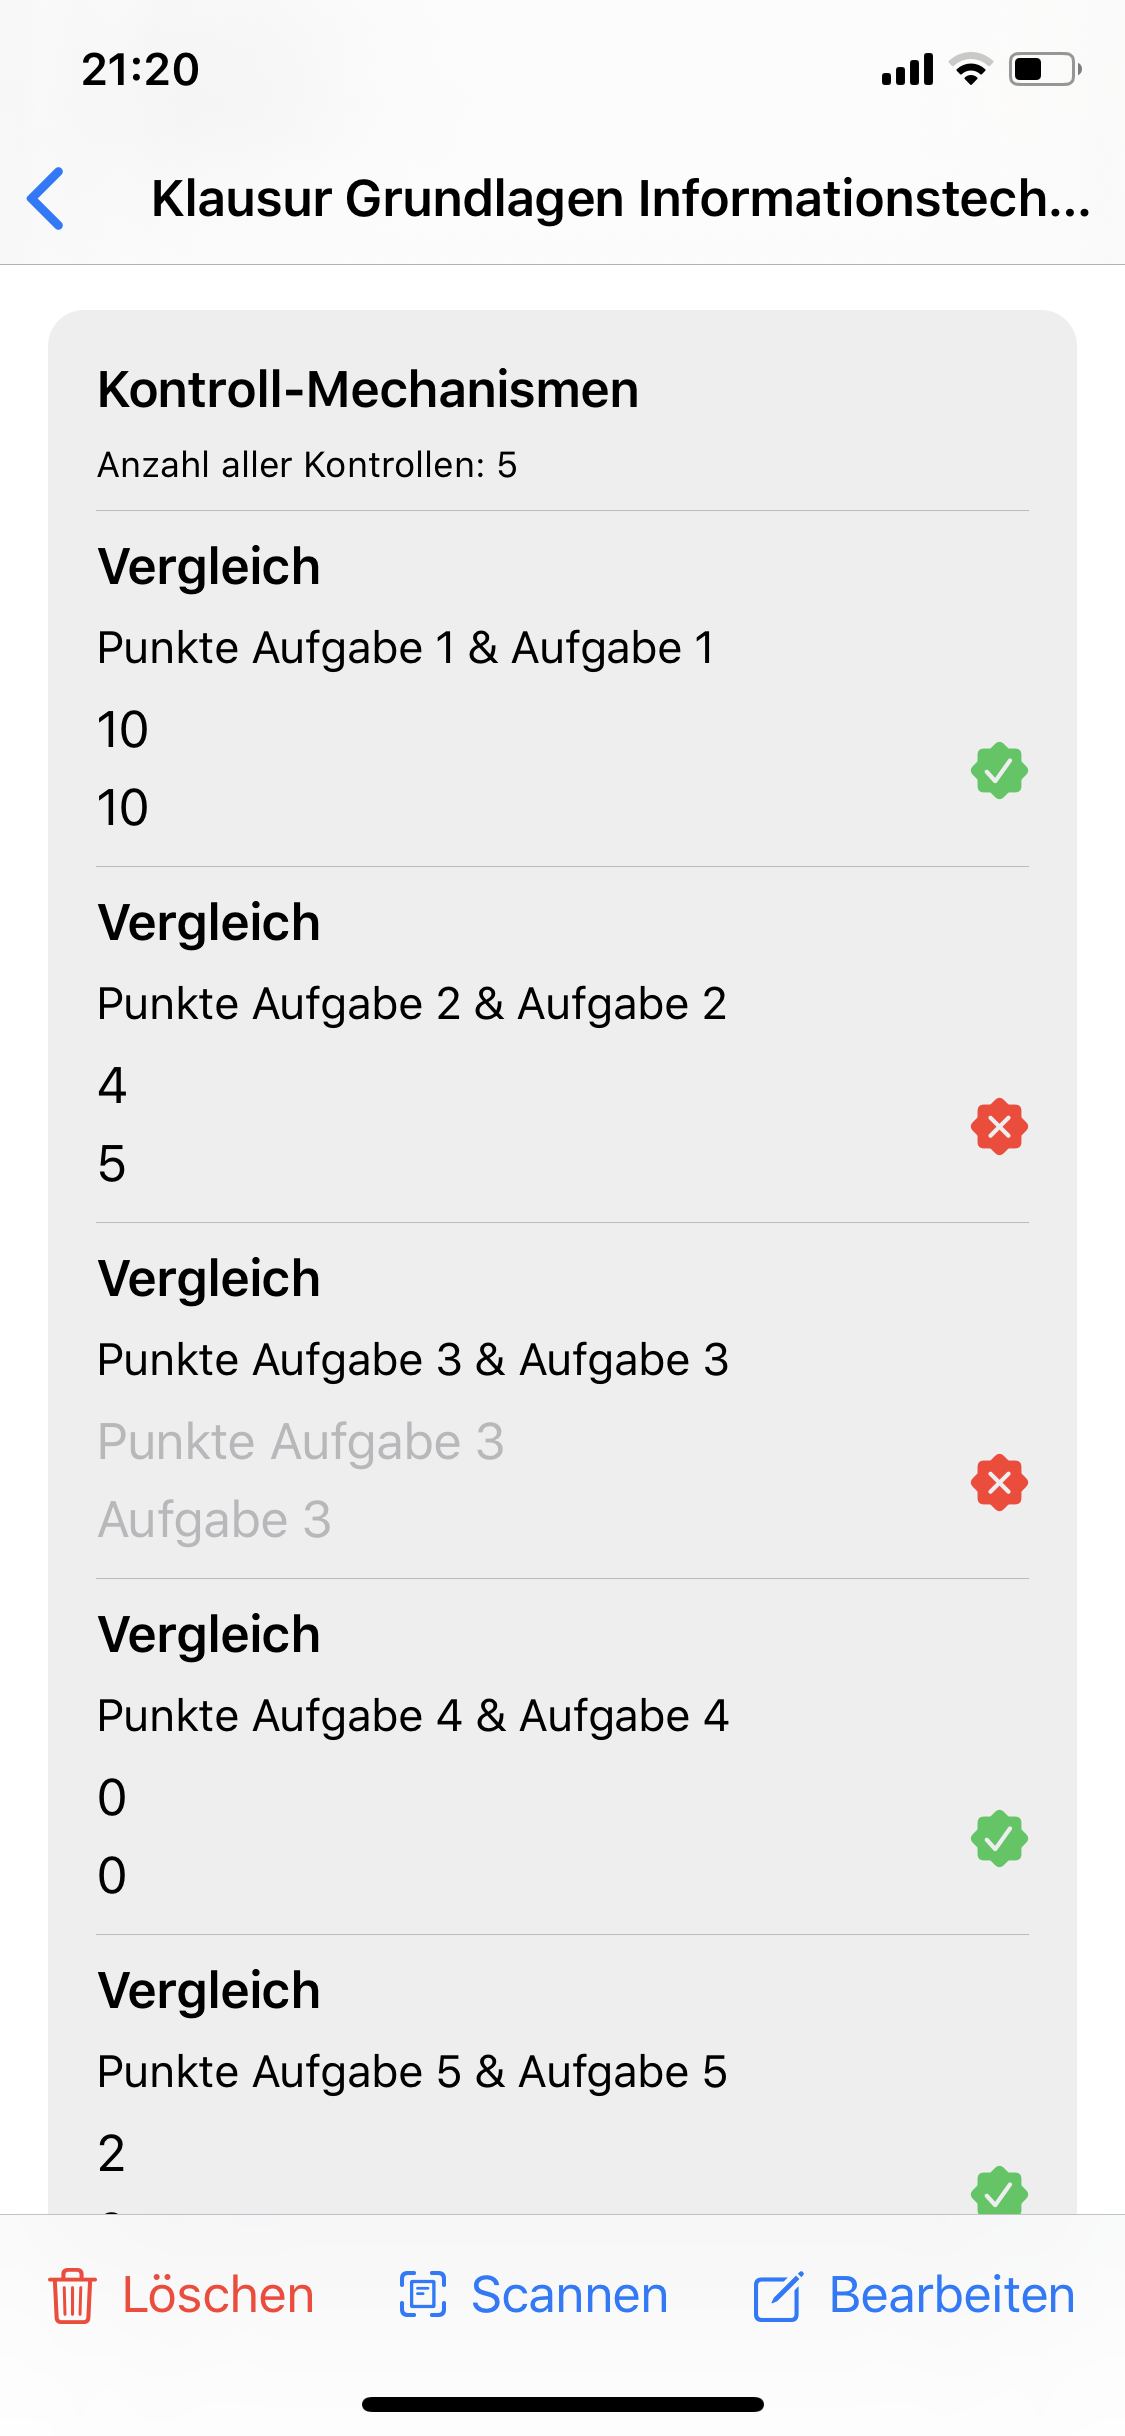
\includegraphics[width=0.96\textwidth]{img/ocr4}}
        			\caption{Dialogfenster zur Auswahl der OCR-Engine}
        			\label{fig:ocr4}
    			\end{subfigure}
    			\caption{Listen- und Detail-Ansicht von Scan-Vorlagen}
				\label{fig:ocr}
			\end{figure}
 
			\subsubsection*{Ablauf mit Tesseract}
				Die Texterkennung mit Tesseract folgenden Ablauf:
				\vspace{-5mm}
				\begin{enumerate}
					\item Bilder an den Server senden.
					\item Auftrag zur Texterkennung an den Server senden.
					\item Serverseitige Texterkennung durchführen.
					\item Texterkennungsergebnisse empfangen und darstellen.
				\end{enumerate}
				
				\paragraph*{Zu 1.: Bilder an den Server senden.}
				Nachdem das Dokument fotografiert wurde, werden die Aufnahmen an den Server gesendet. Dieser gibt die Speicherpfade der Bilder als Antwort zurück. 
				
				\paragraph*{Zu 2.: Auftrag zur Texterkennung an den Server senden.}
				Anschließend wird für jeden Pfad ein Auftrag zur Texterkennung an  die OCR-Schnittstelle des Servers ausgelöst. In der Anfrage wird der Pfad des Bildes und die passende Seiten-ID der ausgewählten Vorlage gesendet. Nun übernimmt der Server die Arbeit der Texterkennung.
				
				\paragraph*{Zu 3.: Serverseitige Texterkennung durchführen.}
				Mithilfe der Seiten-ID, die in der Datenbank des Servers hinterlegt ist, werden die Regionen der Seite auf das Bild, welches sich an dem gesendeten Pfad befindet, angewendet. Für mehr Details siehe im Praktikumsbericht von Tobias Kallauke. 
				
				\paragraph*{Zu 4.: Texterkennungsergebnisse empfangen und darstellen.}
				Nach der Texterkennung sendet der Server die Ergebnisse der Seiten als Antwort zurück. Wie bei Vision werden diese im selben State des State-Containers gesichert. Die Ergebnisse bestehen aus der Region-ID zur Zuordnung, dem erkannten Text sowie der confidence des OCR zum jeweiligen Text. Ähnlich, wie bei Vision.      

%%%%%%%%%%%%%%%% - FAZIT - %%%%%%%%%%%%%%%

\chapter{Fazit}\label{ch:fazit}
	Dieses Kapitel reflektiert den aktuellen Stand der App und zieht einen Vergleich mit den Anforderungen aus \autoref{ch:anforderungen}. Im Anhang \autoref{ch:accses} sind dazu einige weitere Screenshots abgebildet.
	
	\section{Stand des Prototyps}
		Während der Entwicklung konnten die meisten Funktionen des Prototyps umgesetzt werden. Jedoch fehlt zum Zeitpunkt der Abgabe ein essentieller Bestandteil der App. Auf Grund mangelnder Zeit war es nicht mehr möglich, die Funktion zum Speichern der digitalisierten Daten in Front- und Backend zu implementieren. Auch fehlt die Überführung der Daten in ein geeignetes Format.
		
		Außerdem sind nicht alle verfügbaren Serverschnittstellen implementiert. Die Views zum Ändern einer Scan-Vorlage sind schon integriert, da die Views zum Erstellen einer Scan-Vorlage hier wieder verwendet werden konnten. Es fehlen lediglich die interne Logik sowie Schnittstellen zum Server.	
		
		Weiterhin konnte nur einer der Kontrollmechanismen umgesetzt werden, da zu wenig Zeit in die Planung investiert wurde. Grundsätzlich ließen sich die fehlenden Mechanismen recht schnell implementieren, jedoch ist die aktuelle Datenstruktur nicht zum Speichern in der Datenbank geeignet. Sobald Änderungen an der Datenstruktur vorgenommen werden, kann es zu Fehlern kommen. Es existiert aber schon eine Idee zur Verbesserung. Dafür müssten allerdings neben der App auch der Server und die Datenbank angepasst werden. 
		
		Des Weiteren wurden Fehlermeldungen und/oder -behandlungen bezüglich des Servers nur sporadisch implementiert. Aber auch hierfür sind die Grundlagen schon gelegt, da Fehler stets aufgefangen und zentral abgelegt werden. 
	
%	\section{Hürden während der Entwicklung}
%	
%	- ein paar Worte, wie gut die Entwicklung lief (Simulator vs. echtes Gerät), wo sind die Grenzen des Simulators (Keine Kamera), wo waren Probleme mit dem echten Gerät...
%	
%	
%	- jwt in KeyChain gesichert speichern 
%	
%	- GitHub actions
%	
%	- Debugging bei nicht statischen Daten schwer, Mock erstellen
%	
%	- Umfang von SwiftUI viele Umwege 

	\section{Probleme und Grenzen der App}\label{sc:grenzen}
		In diesem Abschnitt werden eventuell auftretende Probleme benannt und Lösungsvorschläge gegeben.

		\subsection{Probleme beim Erkennen von Dokumenten}\label{ssc:erkennen}
			Beim Fotografieren der Klausuren können infolge mangelnder Belichtung, schlechtem Hintergrund oder durch umgeknickte bzw. verdeckte Ecken, die Seitenränder und/oder die Ecken nicht ausreichend erkannt werden. Die Segementier-Algorithemen stoßen bei der Bildverarbeitung hier an ihre Grenzen. Auf die Erklärung der genauen Hintergründe wird in diesem Bericht verzichtet. Weiterhin kommt es bei schnellen Bewegungen der Kamera oder zu flachem Winkel zum Dokument dazu, dass die App einen falschen Bildausschnitt wählt.
			\vspace{-5mm}
			\begin{itemize}
				\item Die erste Problemlösung besteht darin, einen Blitz zu verwenden. Meistens schaltet sich bei zu wenig Licht die zusätzliche Belichtung automatisch ein. Grundsätzlich empfiehlt es sich aber, immer eine Blitz zu verwenden, da dadurch das Dokument gleichmäßig belichtet wird. Bei einer zu starken Grundbelichtung verschlechtert ein Blitz jedoch das Ergebnis, da Text und Kanten unkenntlich gemacht werden. Um eine gute Qualität zu erzielen, ist es am günstigsten die Dokumente bei Tageslicht und mit Blitz aufzunehmen. 
				\item Weiter ist es möglich die Dokumentenseite noch einmal zu fotografieren oder diese im Bild manuell auszurichten. Dafür stellt VisionKit eine besondere View zur Verfügung, die es dem Benutzer ermöglicht, die Ecken des Dokumentes per Hand auszuwählen.
			\end{itemize}
		
		\subsection{Probleme der Klausur-Vorlage beim Scannen}\label{ssc:problemevorlage}
			Dieser Abschnitt bezieht sich ausschließlich auf bestehende Probleme mit den Klausurseiten, welche in \autoref{fig:klausur} zu sehen sind und während des Praktikums genutzt wurden. Sie stehen stellvertretend für Klausuren-Vorlagen der Fakultät CB. Im \autoref{sc:vorlage}, werden mögliche Änderungen und Lösungen zu den hier aufgeführten Problemen diskutiert.
		
			Wie in der \autoref{fig:seite1} zu sehen ist, wird nicht klar zwischen einem Feld für den Vornamen und Nachnamen differenziert. Zudem ist ein einzelner Strich als Feldbegrenzung ungeeignet. Die Punktefelder in der Tabelle dagegen sind besser abgegrenzt, jedoch zu klein. Die geringe Größe verleitet dazu, das Feld komplett auszunutzen und die Ziffer möglichst groß reinzuschreiben. Allerdings sollte eine gewisser Abstand zur Regionbegrenzung für optimale Texterkennung gelassen werden. Bei dem Notenfeld dagegen existiert keine Begrenzung. Für das Markieren der Region ist das ebenfalls ungeeignet (\ref{fig:v9}). Denn hinter der Note wird die Unterschrift des Prüfers gesetzt, welche bei der Digitalisierung nicht mit erscheinen darf.

		\subsection{Weitere Probleme der App}
			Obwohl SwiftUI die Entwicklung des Prototyps erst möglich gemacht hat, bringt das Framework von Juni 2019 einige Schwierigkeiten mit sich. Seit der Veröffentlichung existiert eine sehr kleine und unvollständige Dokumentation der SwiftUI-Schnittstellen. Auch ist der geringe Umfang von SwiftUI nicht mit dem von UIKit, welches seit Jahren in der iOS-Entwicklung als Standard benutzt wird, zu vergleichen. Das führt immer wieder zu einigen provisorischen Lösungen und macht das Auffinden von Fehlern besonders schwierig. Es kann daher bei der Benutzung der App zu unerwarteten Abstürzen oder Aufhängern kommen. Des Weiteren sind die verwendeten Texterkennung-Engines nur für gedruckte Schrift ausgelegt. Druckschrift wird daher häufiger erkannt als Schreibschrift. Auch bei bestimmten Ziffern, wie 1, 4 und 7 kommt es zu Fehlern bzw. Verwechslungen.
	
	%%%%%%%%%%%%%%%% - TEMPLATES - %%%%%%%%%%%%%%%

	\section{Verbesserung der Klausuren-Vorlage}\label{sc:vorlage}
		Basierend auf der gesammelten Erfahrung mit der Anwendung beschäftigt sich dieser Abschnitt mit Verbesserungs- und Änderungsvorschlägen der Klausur in \autoref{fig:klausur}. Sie steht, wie auch zu vor, stellvertretend für die Klausuren-Vorlagen der Fakultät CB. Alle folgenden Vorschläge haben den Hintergrund, die App bei der Digitalisierung zu unterstützen und beziehen sich auf die in \autoref{sc:grenzen} beschriebenen Probleme.
	
		Der erste Vorschlag bezieht sich auf die große Bedeutung der Ecken und Kanten bei der Erkennung des Dokuments. Diese wichtigen Referenzpunkte werden aber unter bestimmten Bedingungen, wie im \autoref{ssc:erkennen} erklärt, nicht immer erkannt. Deshalb empfiehlt es sich, eigene Referenzpunkt auf dem Dokument anzubringen. Beispielsweise durch einen Rahmen, wie es auf der Klausur (\ref{fig:seite1}) zu sehen ist. oder durch ein QR-Code ähnliches Muster. Ein Vorteil bei eigenen Referenzpunkten ist, dass sich ihre Gestallt immer vom Dokument abheben kann. Somit ist die Dokumenten-Erkennung nur noch vom Licht abhängig. Dadurch kann die Kamera näher an den Text heran, wodurch sich die Bildqualität verbessert. Jedoch kann nun die Erkennung nicht mehr von Frameworks übernommen werden. Es müssten künstliche neuronale Netze trainiert werden, welche diese Referenzpunkte in Bildern erkennen. 
	
		Der zweite Vorschlag bezieht sich auf den \autoref{ssc:problemevorlage}. Dementsprechend wäre es sinnvoll alle Felder ausreichend zu beschriften und mit einer dünnen Linie zu begrenzen. Mithilfe von Bildverarbeitungsalgorithmen könnten die feinen Rahmen ohne Verlust der wichtigen Daten heraus gerechnet werden.
		
		Abschließend ist zu erwähnen, dass laut der Problemstellung aus \autoref{ch:problemstellung} eine Klausuren-Vorlage entwickelt werden sollte. Auf Grund mangelnder Zeit war das jedoch nicht möglich.

%%%%%%%%%%%%%%%% - AUSBLICK - %%%%%%%%%%%%%%%
		
% Jedoch sollten auch einige angesprochenen Probleme aus Kapitel \ref{ch:grenzen} behoben werden, wenn die App in Zukunft tatsächlich von Hochschulmitarbeitern benutzt werden soll.
\chapter{Ausblick}\label{ch:ausblick}
	In den folgenden Abschnitten werden einige Ideen erläutert, wie die App und das gesamte Software-System verbessert werden können.
	
	\paragraph*{Verbesserung der Benutzerfreundlichkeit und des Workflows} \label{pa:benutzer} 
		Angesichts des Prototyp-Status der App sollten bei einer Weiterentwicklung zu allererst Systemkomponenten implementiert werden, die die Benutzung verbessern. Beispielsweise werden Login-Daten und schon heruntergeladene Scan-Vorlagen nicht dauerhaft gespeichert. Auch muss zu jeder Region ein Name vergeben werden. Bei genauerer Betrachtung gibt aber auch der Datentyp (\ref{fig:v6}) der Region in den meisten Fällen Auskunft darüber, wie die Region benannt werden sollte (siehe dazu \autoref{fig:v5}). Handelt es sich um den Vor- bzw. Nachnamen, die Matrikelnummer, Seminargruppe oder Note, taucht diese Region auch nur genau einmal in einer Scan-Vorlage auf. Ausschließlich der Datentyp Punkte soll mehrmals vergeben werden können. Daher ist es sinnvoll den Workflow beim Erstellen von Regionen entsprechend anzupassen. 
	
	\paragraph*{Weitere Dokument- und Datentypen} 
		Auf dem \hyperref[pa:benutzer]{Abschnitt Verbesserung der Benutzerfreundlichkeit und des Workflows} \xspace aufbauend, ist folgende Idee entstanden. Durch die generischen Vorlagen ist es möglich, neben Klausuren auch andere Dokumente nach diesem Schema zu digitalisieren. Beispielsweise Krankenscheine, Urlaubsanträge oder Arbeitsverträge. Dafür könnten spezielle Workflows zum Erstellen der jeweiligen Vorlage und weitere Regionen-Datentypen implementiert werden, wie z. B. Datum, IBAN-Nummer, E-Mailadresse und Telefonnummer.
		
%	\paragraph*{Weitere Kontrollmechanismen} 
%		Typische Mathematische Operatoren, + - / * < > >= <= ( ), Mengenlehre, Datentypen verwenden (Datum > 01.01.2020), Alter > 18
	
	\paragraph*{Erweiterung der Texterkennung} 
		Wie im \autoref{sc:grenzen} erwähnt unterstützen Vision und Tesseract nicht das Erkennen von Schreibschrift. Jedoch wäre es möglich eigene neuronale Netze zu trainieren und implementieren, die diese Aufgabe übernehmen. Beispielsweise existiert ein Datensatz an handgeschriebenen Ziffern \footurl{MNIST-Datensatz -}{http://yann.lecun.com/exdb/mnist/}, mit dem ein einfaches Netz für das Erkennen von Ziffern, trainiert werden kann. Außerdem bietet die Serverarchitektur die Möglichkeit, andere oder mehr OCR-Engines zu implementieren. Für mehr Details siehe im Praktikumsbericht von Tobias Kallauke.
	
	\paragraph*{Klausuren-Einsicht} 
		Die archivierten Klausurenbilder könnten über ein Web-Portal dazu genutzt werden, eine Online-Einsicht der Prüfungen zu ermöglichen. Jedoch bringt solch eine Plattform auch ein Problem mit sich. Durch sie ist die Verbreitung von Klausuren noch einfacher als zuvor, wodurch die Professoren dazu angehalten werden, sich immer wieder neue Aufgaben auszudenken. Aber auch dafür könnte es in Zukunft eine Lösung geben. 
	
	\paragraph*{Weitere Plattformen} 
		Neben der iOS-App versuchte Tobias Kallauke dieselbe für die Android-Plattform zu entwickeln. Jedoch existierten zum Zeitpunkt des Praktikums keine passenden Frameworks, die das Erkennen von Dokumenten in Echtzeit übernehmen. Deshalb entwickelte Tobias einen Prototyp, der sich ausschließlich mit diesem Problem beschäftigt. Jedoch könnte das Software-System auf noch mehr Plattformen Anwendung finden. Neben einem Programm für Linux, MacOS und Windows ist auch eine Web-Plattform erdenklich. Alle Plattformen könnten den selben Funktionsumfang besitzen. Lediglich das Erstellen bzw. Aufnehmen der Fotos erfolgt beispielsweise über Scan- oder Kopiergeräte.
	
	\paragraph*{Intelligente Referenzpunkte}\label{pa:referenzpunkte}
		In \autoref{sc:vorlage} wurde erwähnt, dass eigene Referenzpunkte auf den Klausuren Vorteile mit sich bringen. Möglich wäre auch, dass die Referenzpunkte ähnlich wie QR-Codes aufgebaut sind. Diese enthalten die nötigen Informationen zu den Regionen auf der Seite und ermöglichen das Digitalisieren ohne die Auswahl der richtigen Vorlage. Daran angelehnt könnten ein \LaTeX -Paket oder Word-PlugIn entwickelt werden, wodurch die QR-Codes automatisch für jede Seite und deren Regionen generiert werden. 
	
	\paragraph*{Klausuren-Vorlage entwickeln}
		Auf \autoref{sc:vorlage} und den \hyperref[pa:referenzpunkte]{intelligenten Referenzpunkten} aufbauend könnten eigene Klausuren-Vorlagen umgesetzt und getestet werden. Eine Anpassung der App ist erforderlich, sodass die Referenzpunkte erkannt werden, wie im \autoref{sc:vorlage} beschrieben.
		
	\paragraph*{Benutzerakzeptanzstudie}\label{pa:akzeptanz}
		Aktuell ist unklar, ob die App tatsächlich Zeit einspart. Aus diesem Grund ist es sinnvoll eine umfangreiche Benutzerakzeptanzstudie durchzuführen. Außerdem könnten so weitere Probleme entdeckt und Lösungen entwickelt werden, bevor die App benutzt werden kann.
	
	%\paragraph*{Qualitätsstudie} 
		%Neben einer \hyperref[pa:akzeptanz]{\textit{Benutzer Akzeptanz Studie}} könnte außerdem eine Qualitätsstudie der aktuellen oder auch anderer OCR-Engines erstellt werden. Es gibt viele online OCR-Engines Beispielsweise von Microsoft und Google
	
	%\paragraph*{Versionsverwaltung von Dokumenten} Dokumente an Hochschulen gehen oft durch viele Hände. Dabei werden die Dokumente im schlechtesten Fall immer wieder eingescannt, per E-Mail versendet und wieder ausgedruckt. Das verbraucht nicht nur viele Ressourcen sondern führt hin und wieder auch dazu, das veraltete Versionen des Dokuments weiter gereicht werden. Um all diese Probleme zu vermeiden, könnte eine Versionsverwaltung für Dokumenten entstehen, die auf der App aufbaut. 

\Anhang

\chapter{Wasserfall-Modell}
	\begin{figure}[th]
   		\centering
   		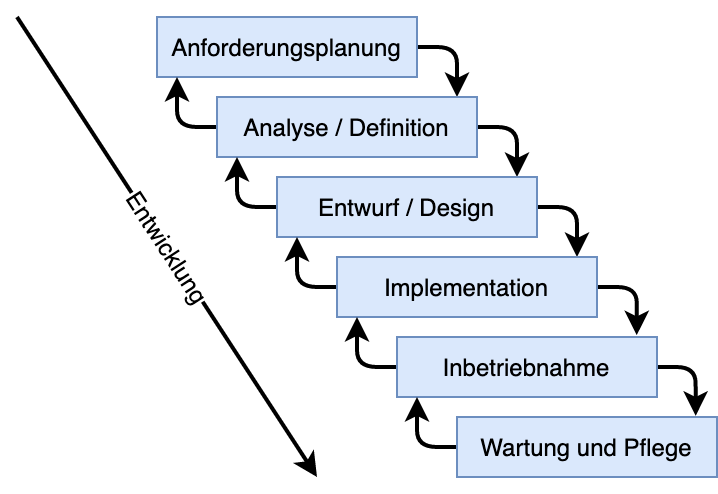
\includegraphics[width=0.7\textwidth]{img/waterfall}
   		\caption{Das Wasserfall-Model nach Winston W. Royce}
   		\label{fig:waterfall}
   \end{figure}

\chapter{Workflow} \label{ch:workflow}
	\section*{Scan-Vorlage erstellen}
	\begin{enumerate}
		\item ''Neue Vorlage erstellen''
		\item Foto machen
		\item Frage: Ist Foto gut?
		\vspace{-5mm}
		\begin{enumerate}
			\item Ja: gehe zu 4.
			\item Nein: gehe zu 2.
		\end{enumerate}
		\item Neues Attribut hinzufügen
		\item Bereich auf Bild auswählen
		\item Frage: Ist Bereich gut?
		\vspace{-5mm}
		\begin{enumerate}
			\item Ja: gehe zu 7.
			\item Nein: gehe zu 5.
		\end{enumerate}
		\item Name für Attribut festlegen
		\item Datentyp für Attribut festlegen (Name, Matrikelnummer, Note, ...)
		\item Frage: Sind alle Attribute vorhanden?
		\vspace{-5mm}
		\begin{enumerate}
			\item Ja: gehe zu 10.
			\item Nein: gehe zu 4.
		\end{enumerate}
		\item Fertig
		\item Vorlage an Server senden
	\end{enumerate}
	
	\begin{figure}[th]
   		\centering
 		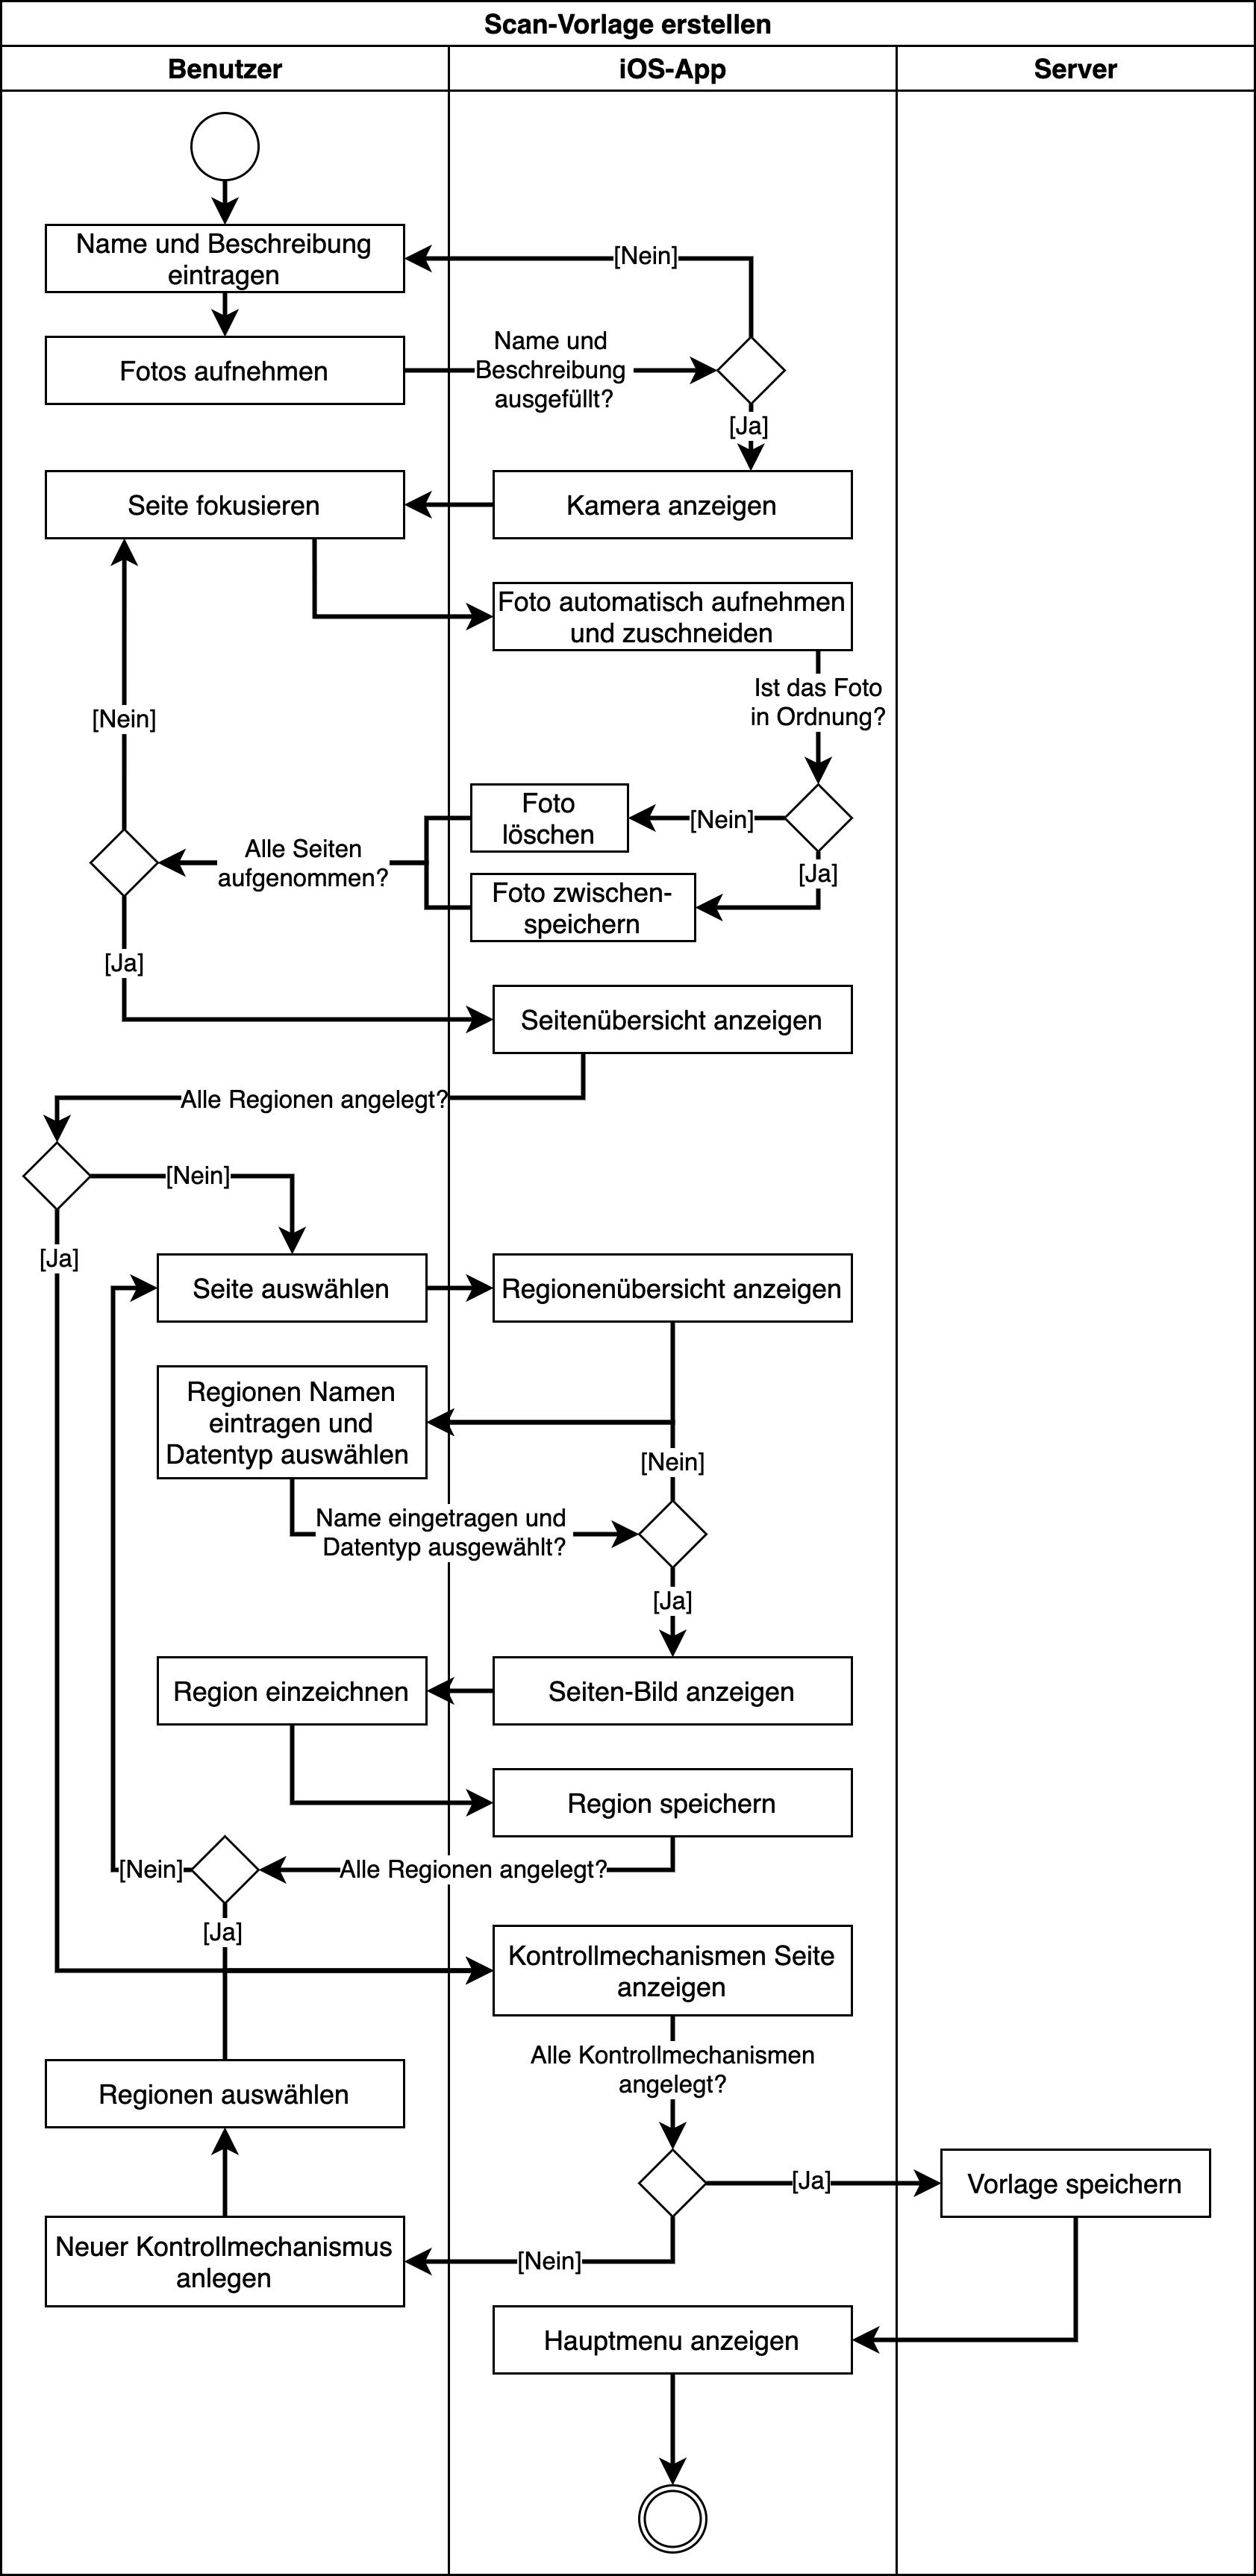
\includegraphics[width=\textwidth,height=\textheight,keepaspectratio]{img/erstellen_flow}
   		\caption{Gekürztes Flussdiagramm zum Erstellen einer Scan-Vorlage}
   		\label{fig:erstellen_flow}
   	\end{figure}
   	
   	\begin{figure}[th]
   		\centering
   		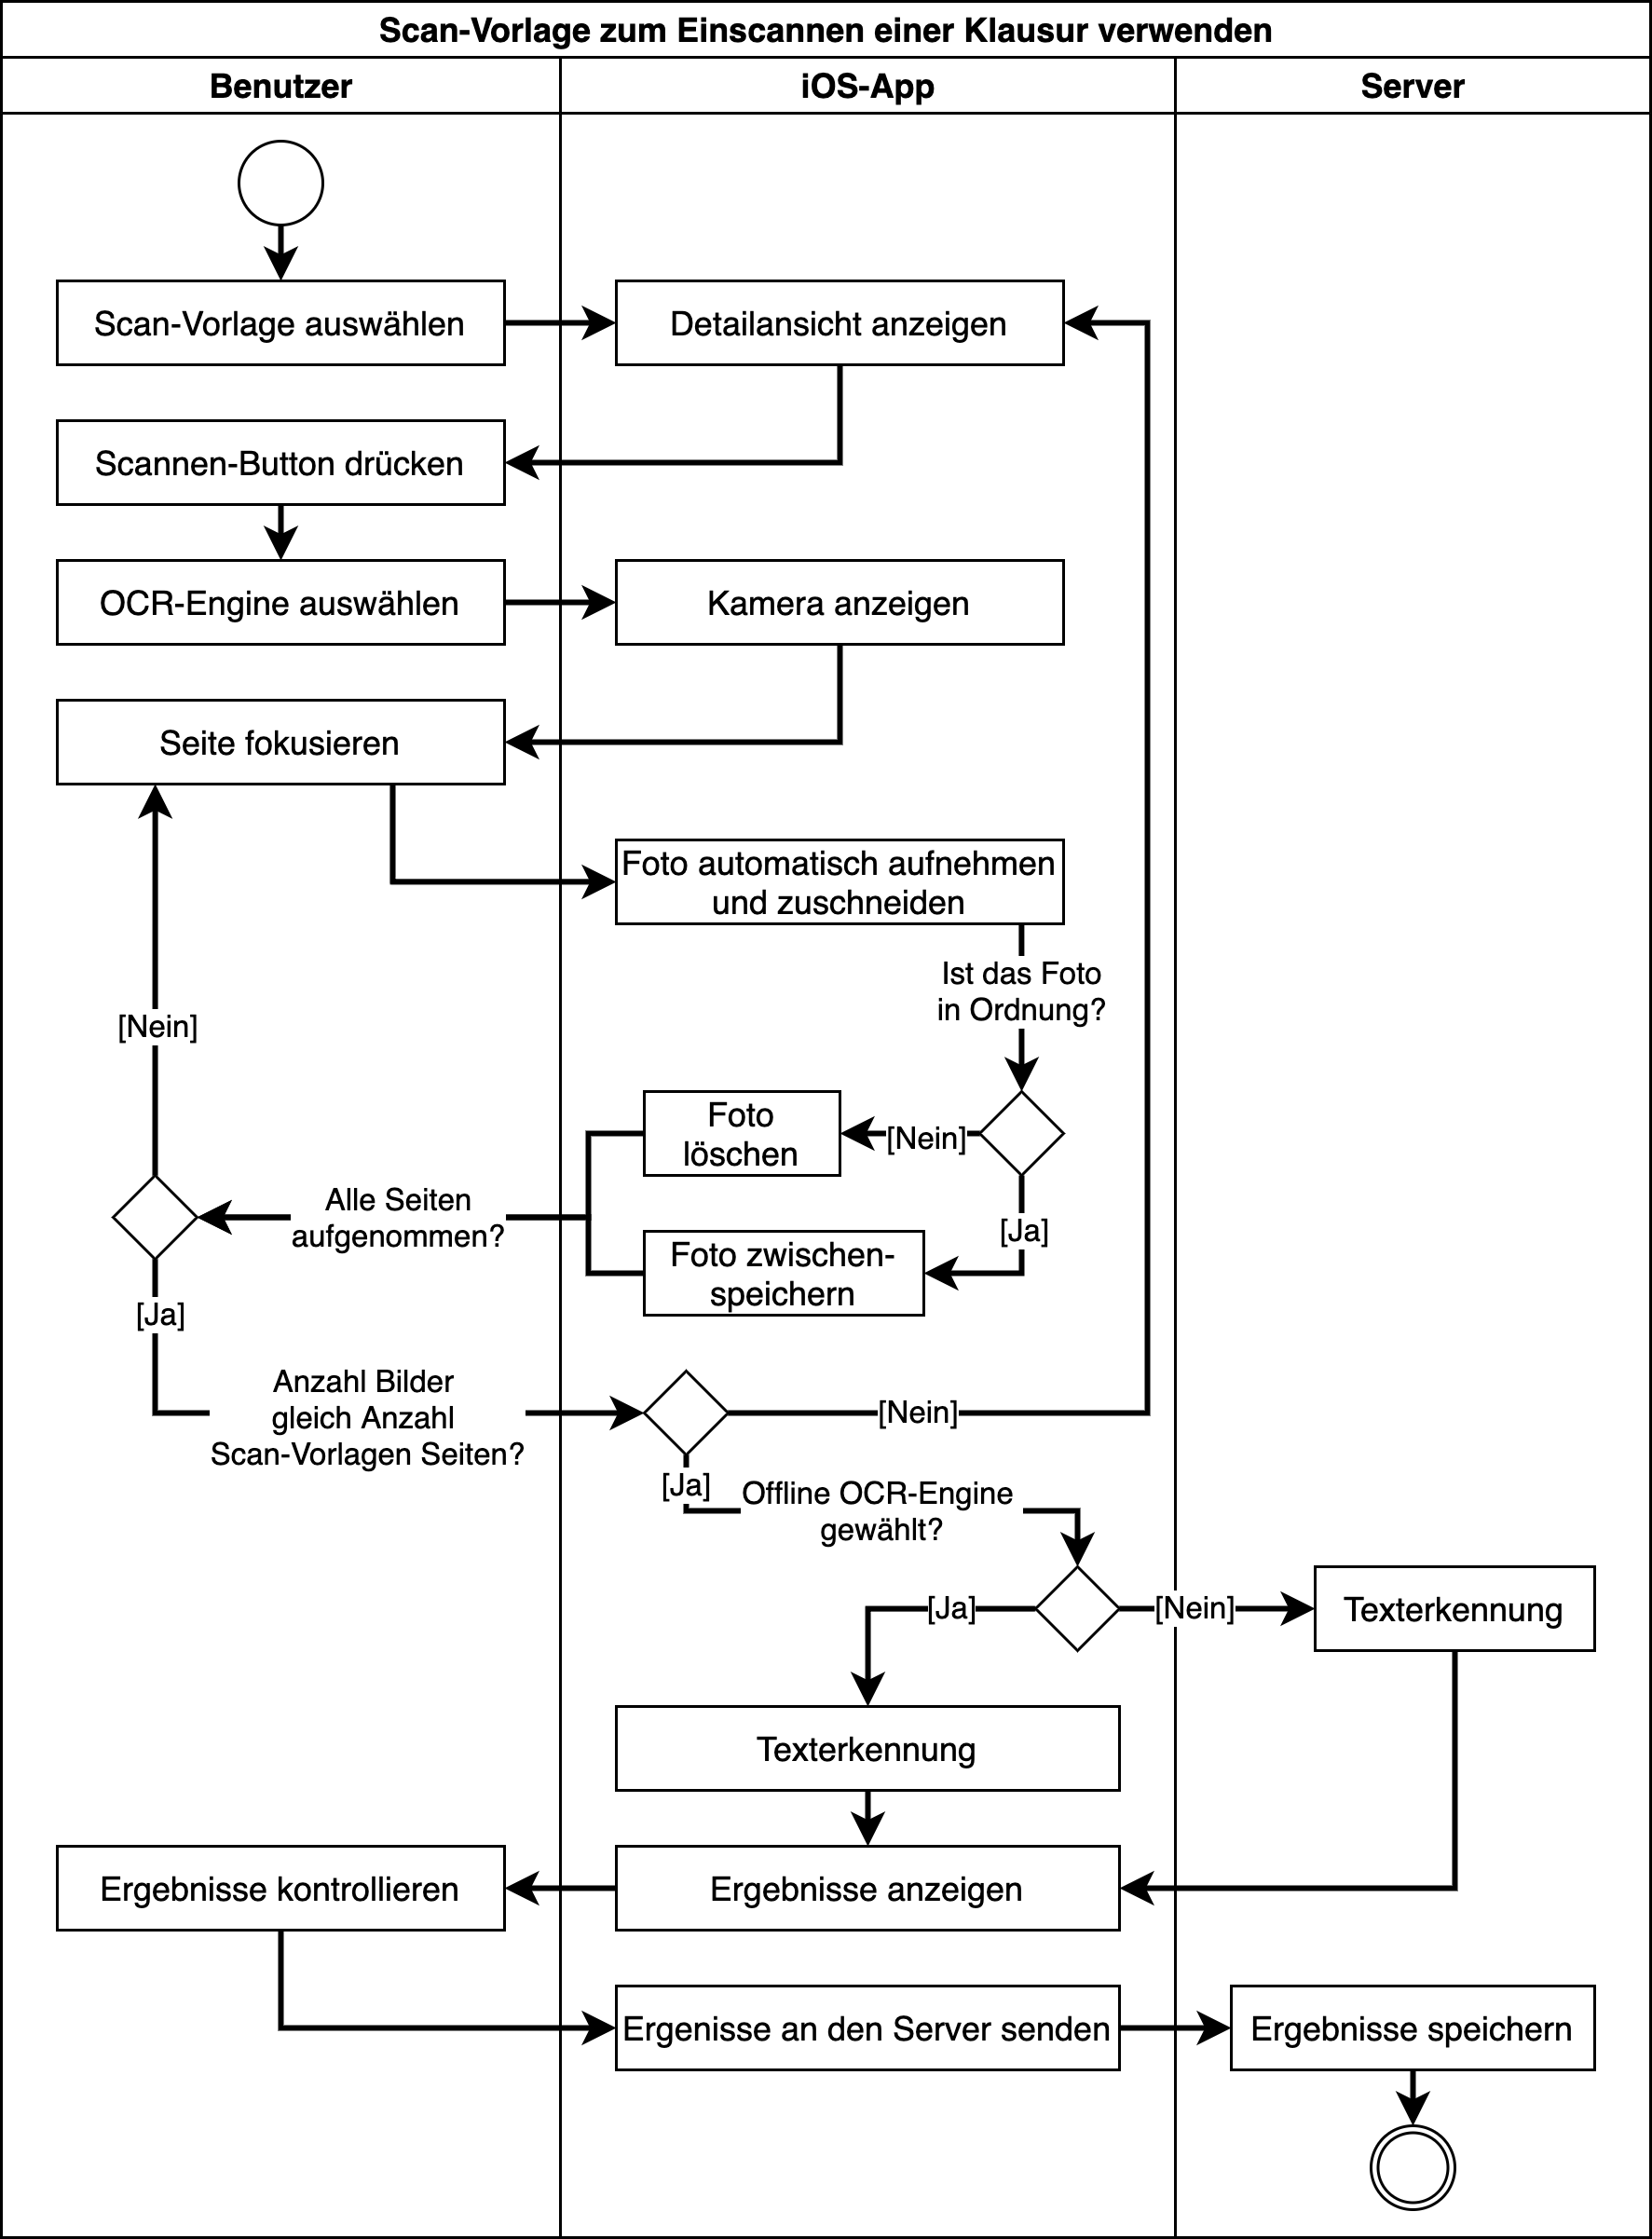
\includegraphics[width=\textwidth,height=\textheight,keepaspectratio]{img/verwenden_flow}
   		\caption{Gekürztes Flussdiagramm zum Verwenden einer Scan-Vorlage}
   		\label{fig:verwenden_flow}
   	\end{figure}

	
\chapter{Weitere Funktionalität} \label{ch:accses}

	\begin{figure}[ht]
	    \centering
		\begin{subfigure}[h]{\textwidth}
		    \frame{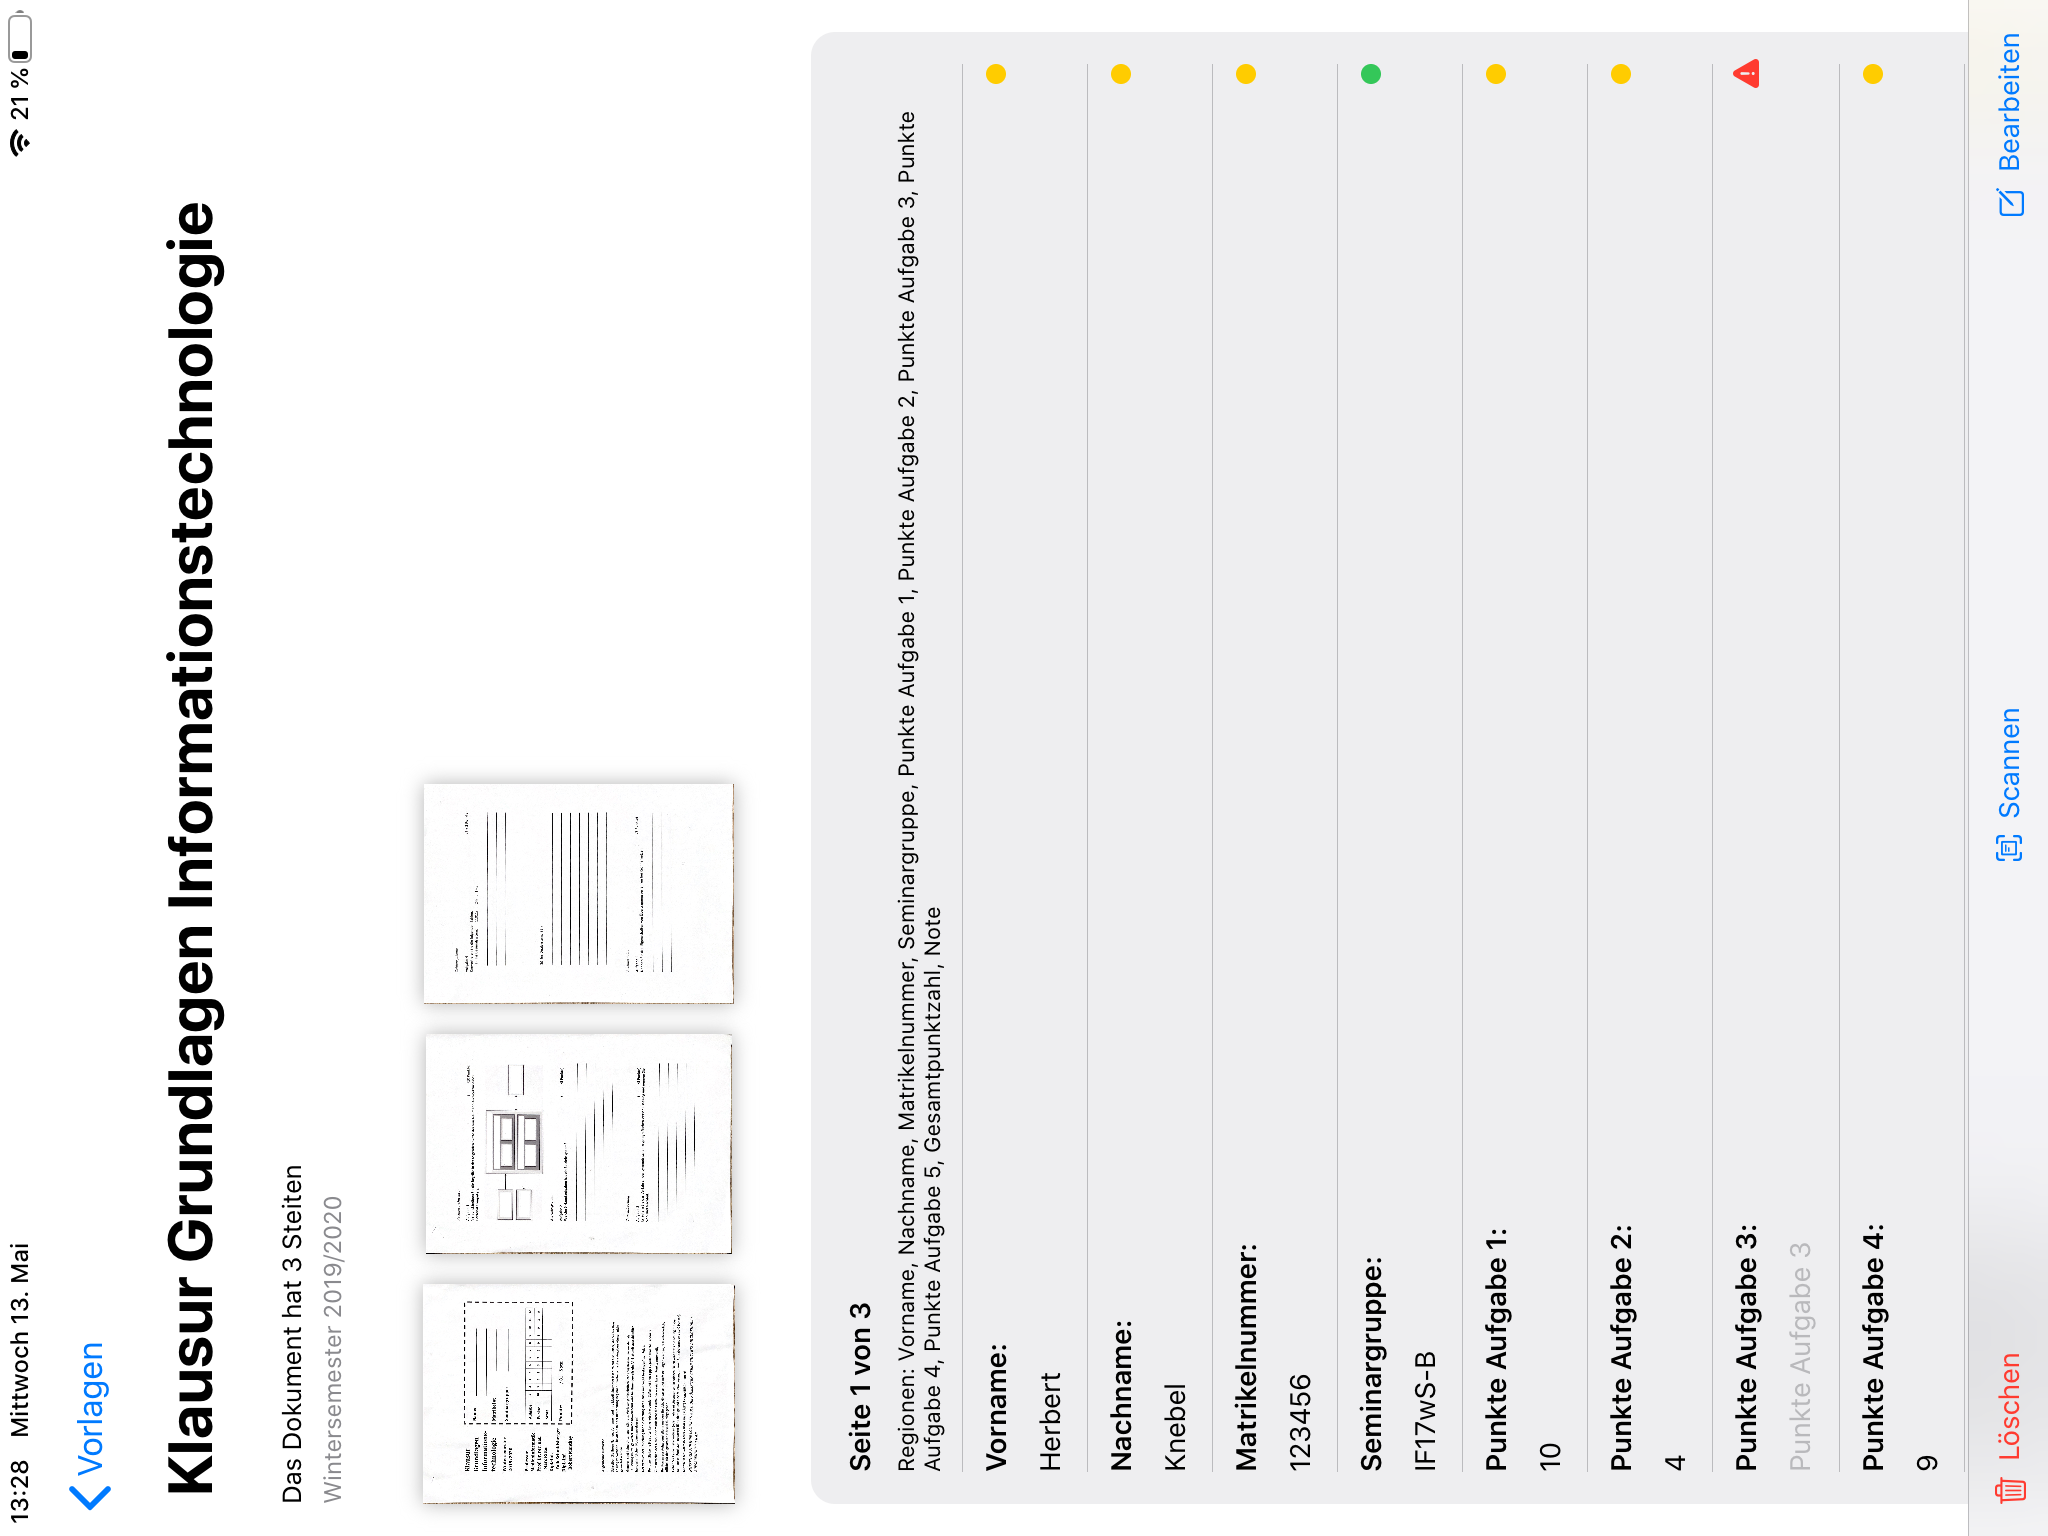
\includegraphics[height=0.3\textheight,keepaspectratio]{img/pad1}}
		    \caption{Ergebnisse ansehen auf dem iPad}
		    \label{fig:pad1}
		\end{subfigure}
		
       	\begin{subfigure}[h]{\textwidth}
		    \frame{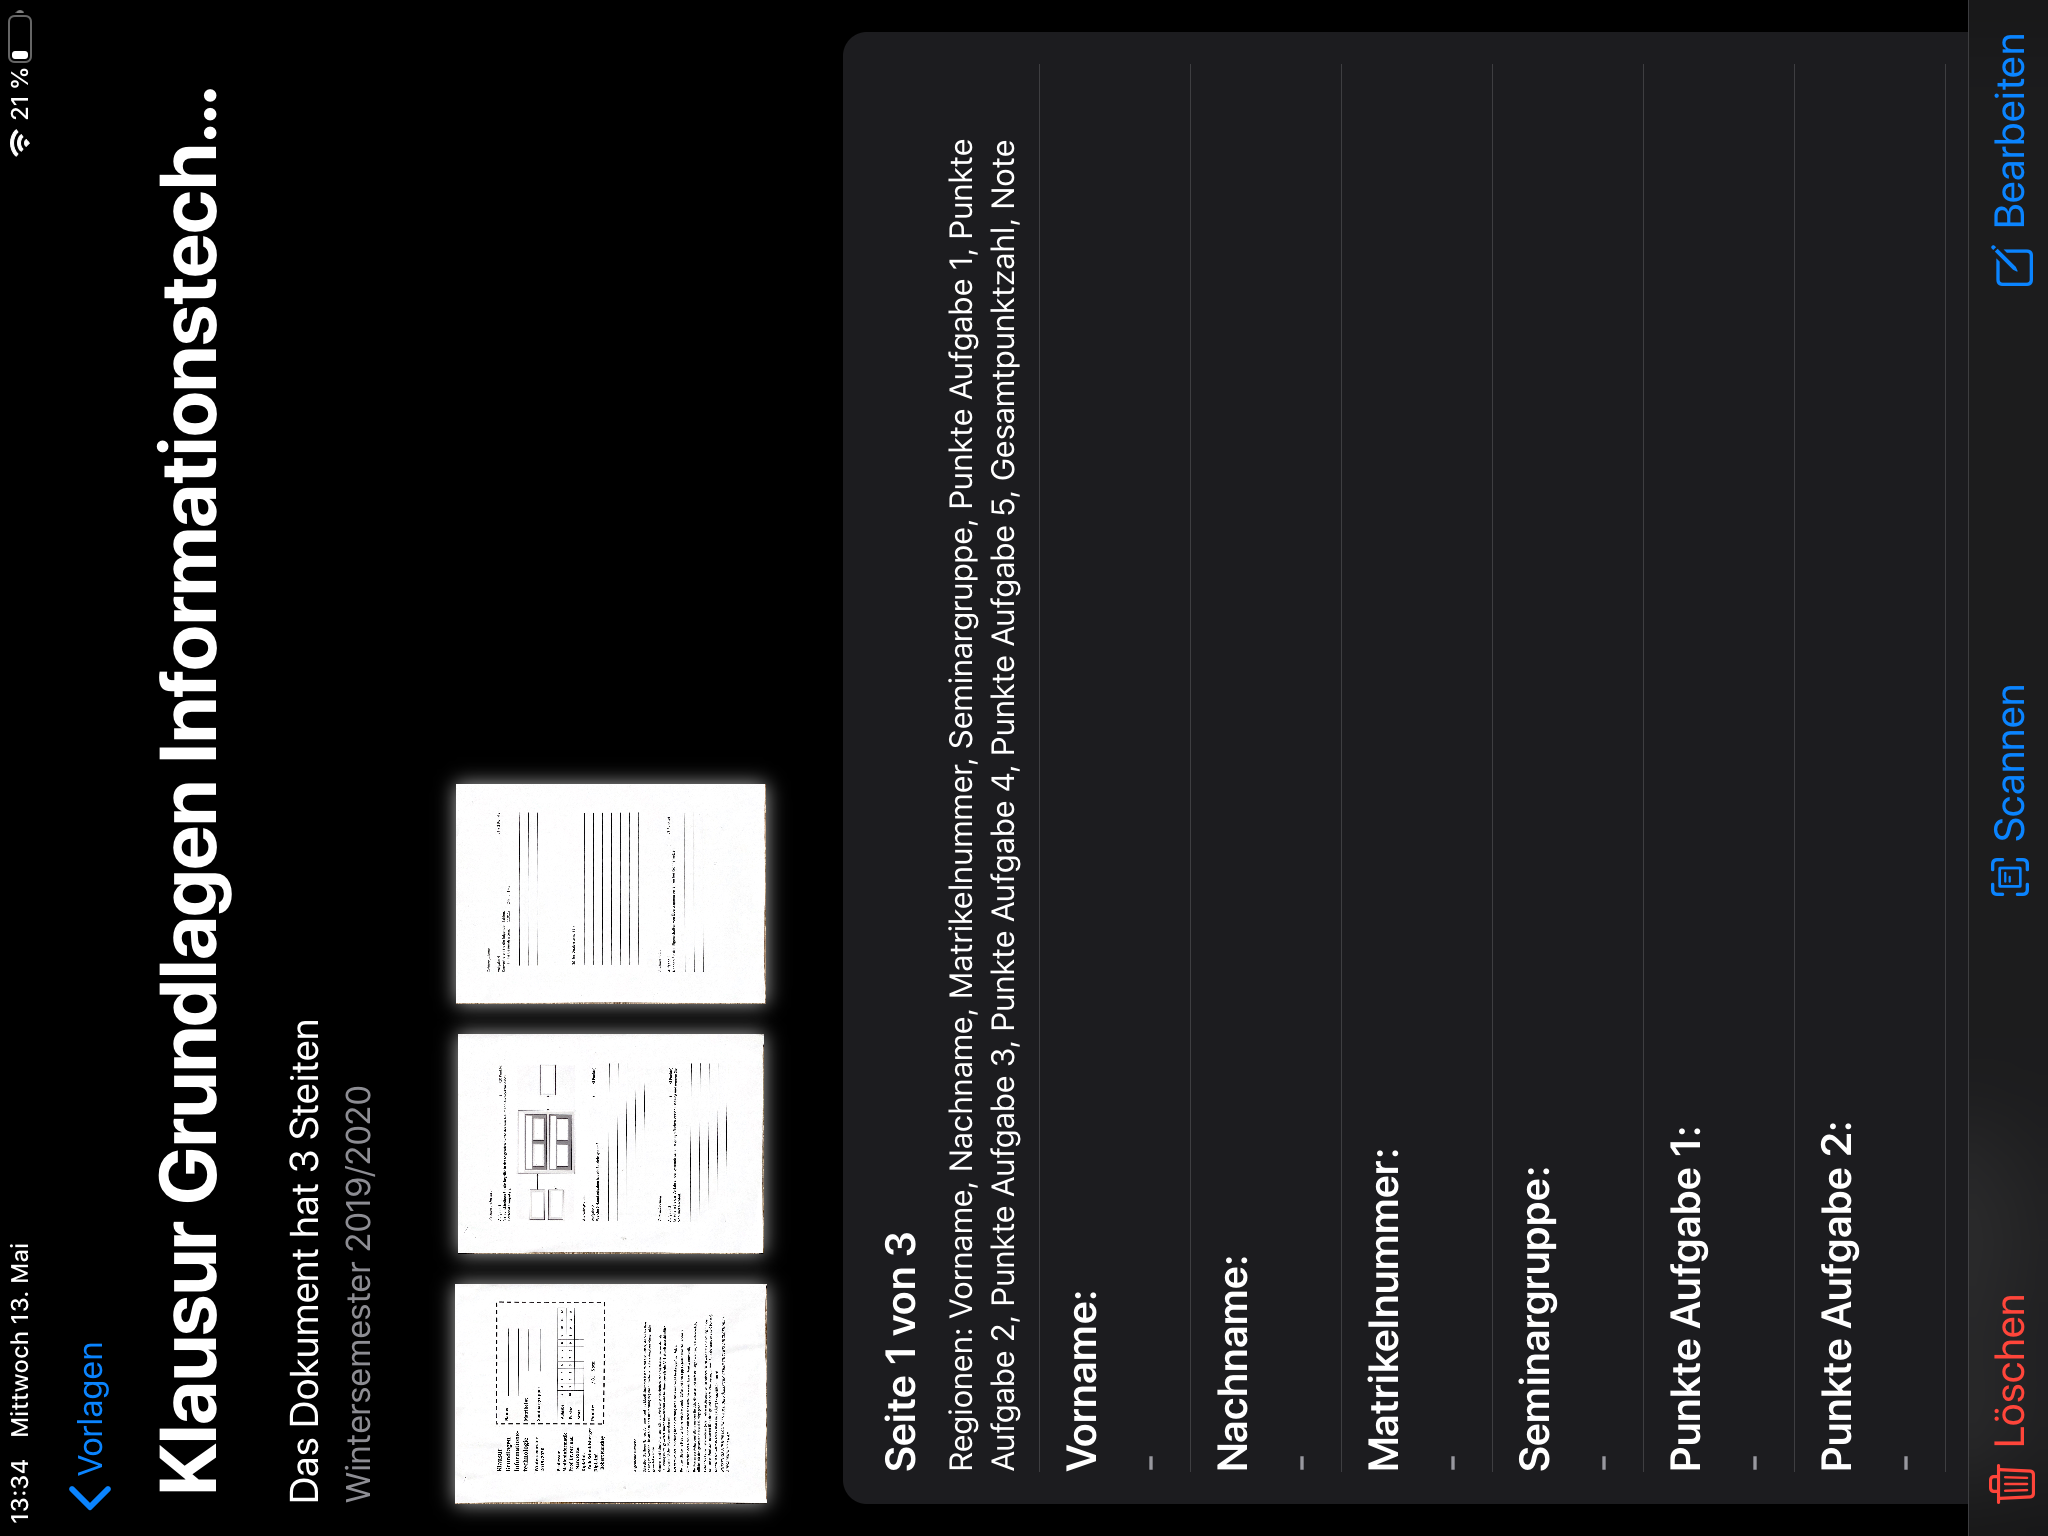
\includegraphics[height=0.3\textheight,keepaspectratio]{img/pad2}}
		    \caption{Vorlagen-Detailansicht mit Dark-Mode und der größten einstellbaren Textgröße}
		    \label{fig:pad2}
		\end{subfigure}
    	\caption{Vorlagen-Detailansicht auf einem iPad mit Barrierefreiheit Beispiel}
		\label{fig:zusatz5}
	\end{figure}
	
	\begin{figure}[h]
		\centering
		\begin{subfigure}[t]{0.3\textwidth}
       		\frame{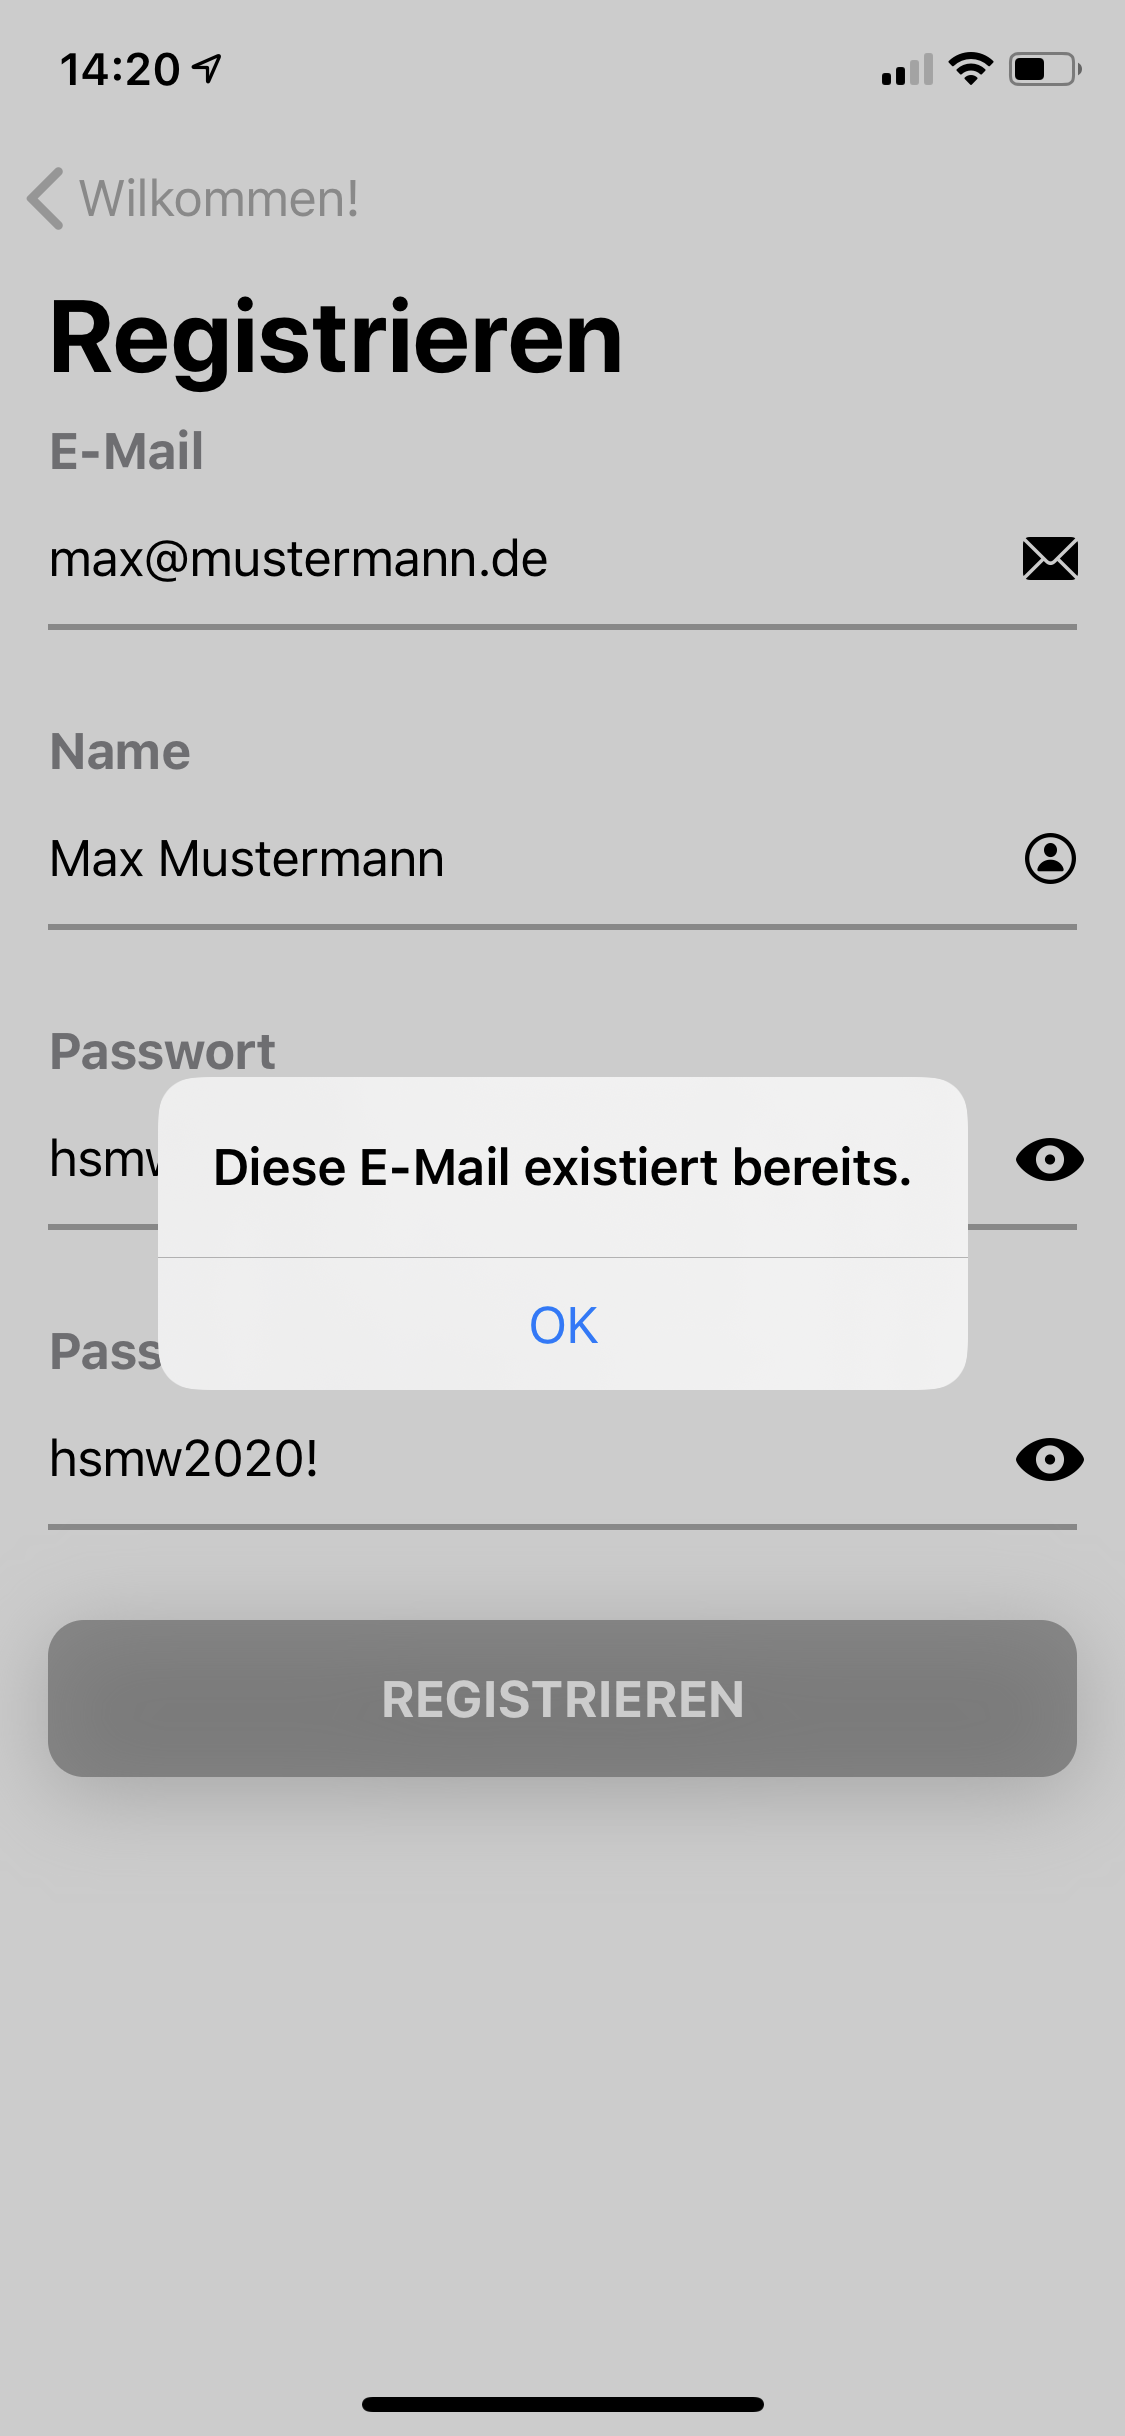
\includegraphics[width=0.96\textwidth]{img/9}}
        	\caption{Eine der integrierten Fehlermeldungen beim Registrieren}
        	\label{fig:9}
    	\end{subfigure}
    	\begin{subfigure}[t]{0.3\textwidth}
       		\frame{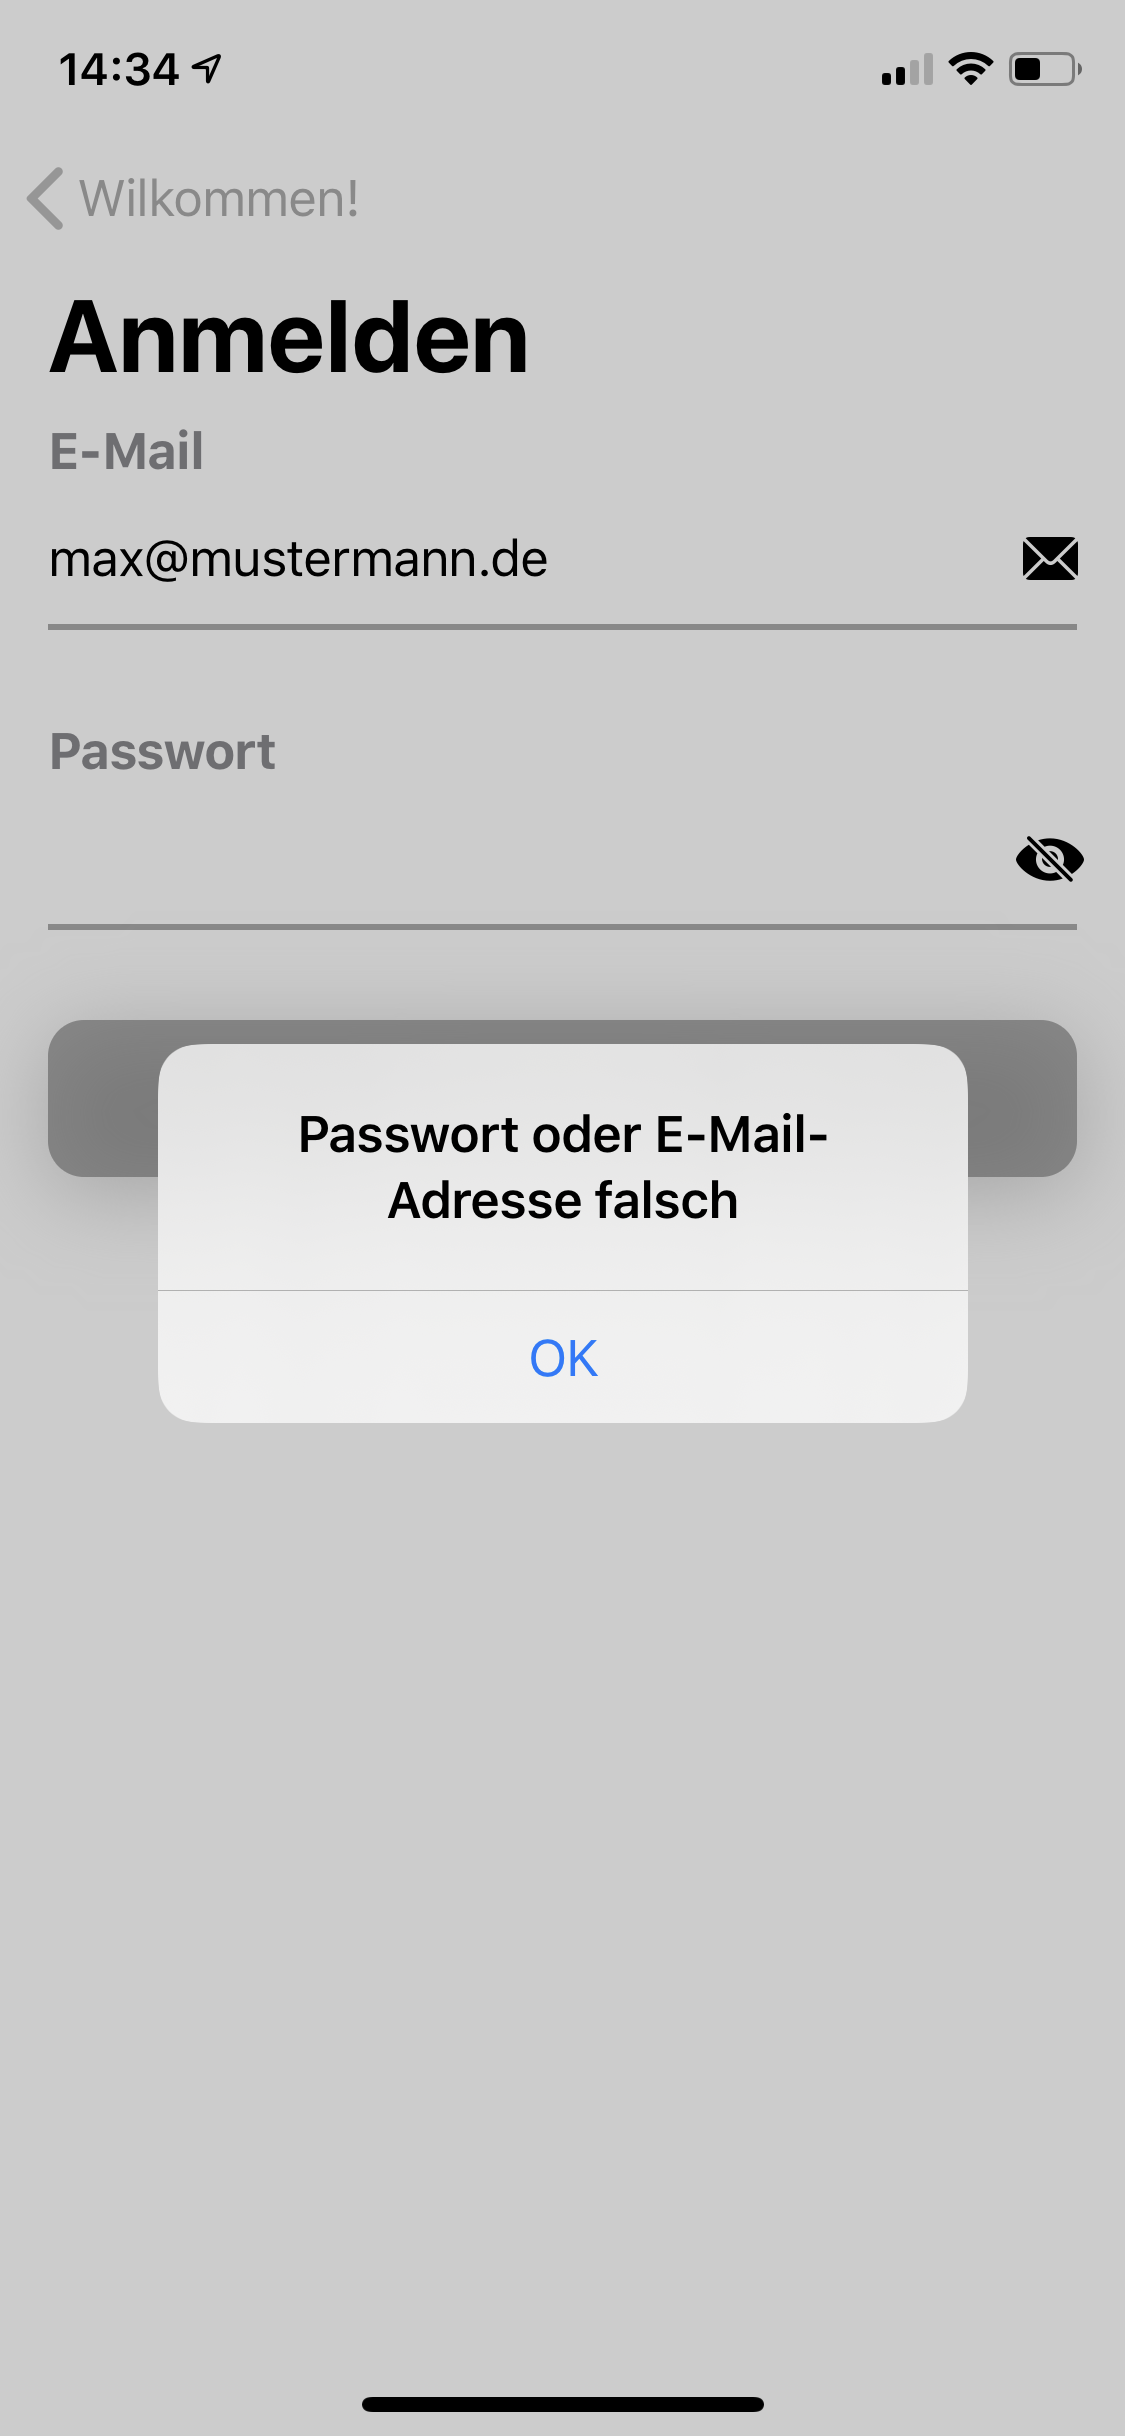
\includegraphics[width=0.96\textwidth]{img/13}}
        	\caption{Eine der integrierten Fehlermeldungen beim Anmelden}
        	\label{fig:13}
    	\end{subfigure}
    	\begin{subfigure}[t]{0.3\textwidth}
       		\frame{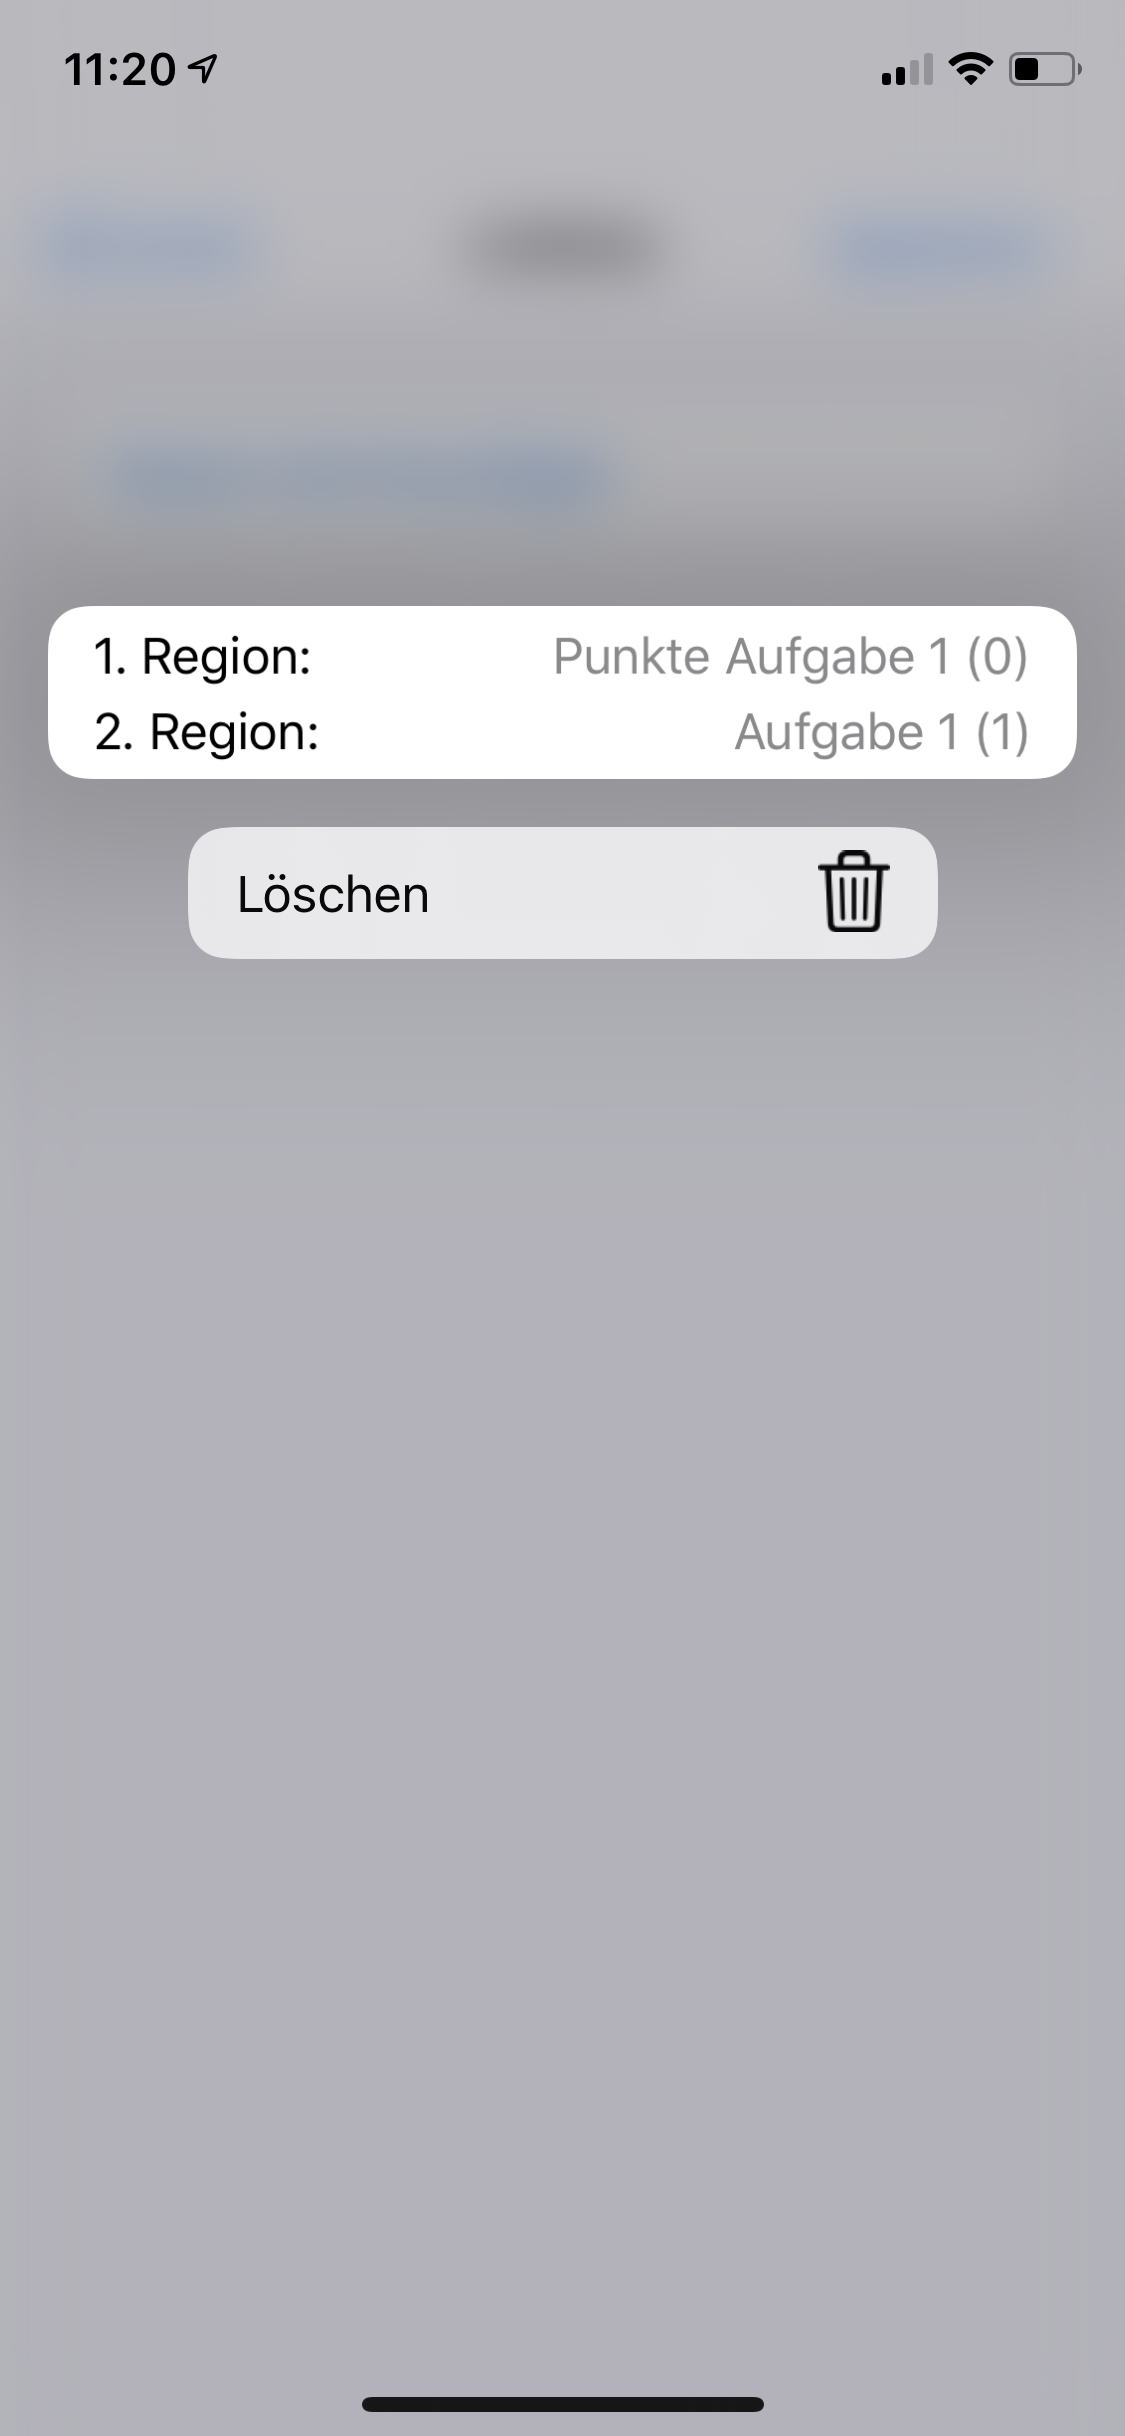
\includegraphics[width=0.96\textwidth]{img/L5}}
        	\caption{Löschen eines angelegten Kontrollmechanismuses}
        	\label{fig:l5}
    	\end{subfigure}
    	\caption{Beispiel-Fehlermeldungen und View beim Löschen eines angelegten Kontrollmechanismuses}
		\label{fig:zusatz2}
	\end{figure}
	
	\begin{figure}[h]
		\centering
		\begin{subfigure}[t]{0.3\textwidth}
       		\frame{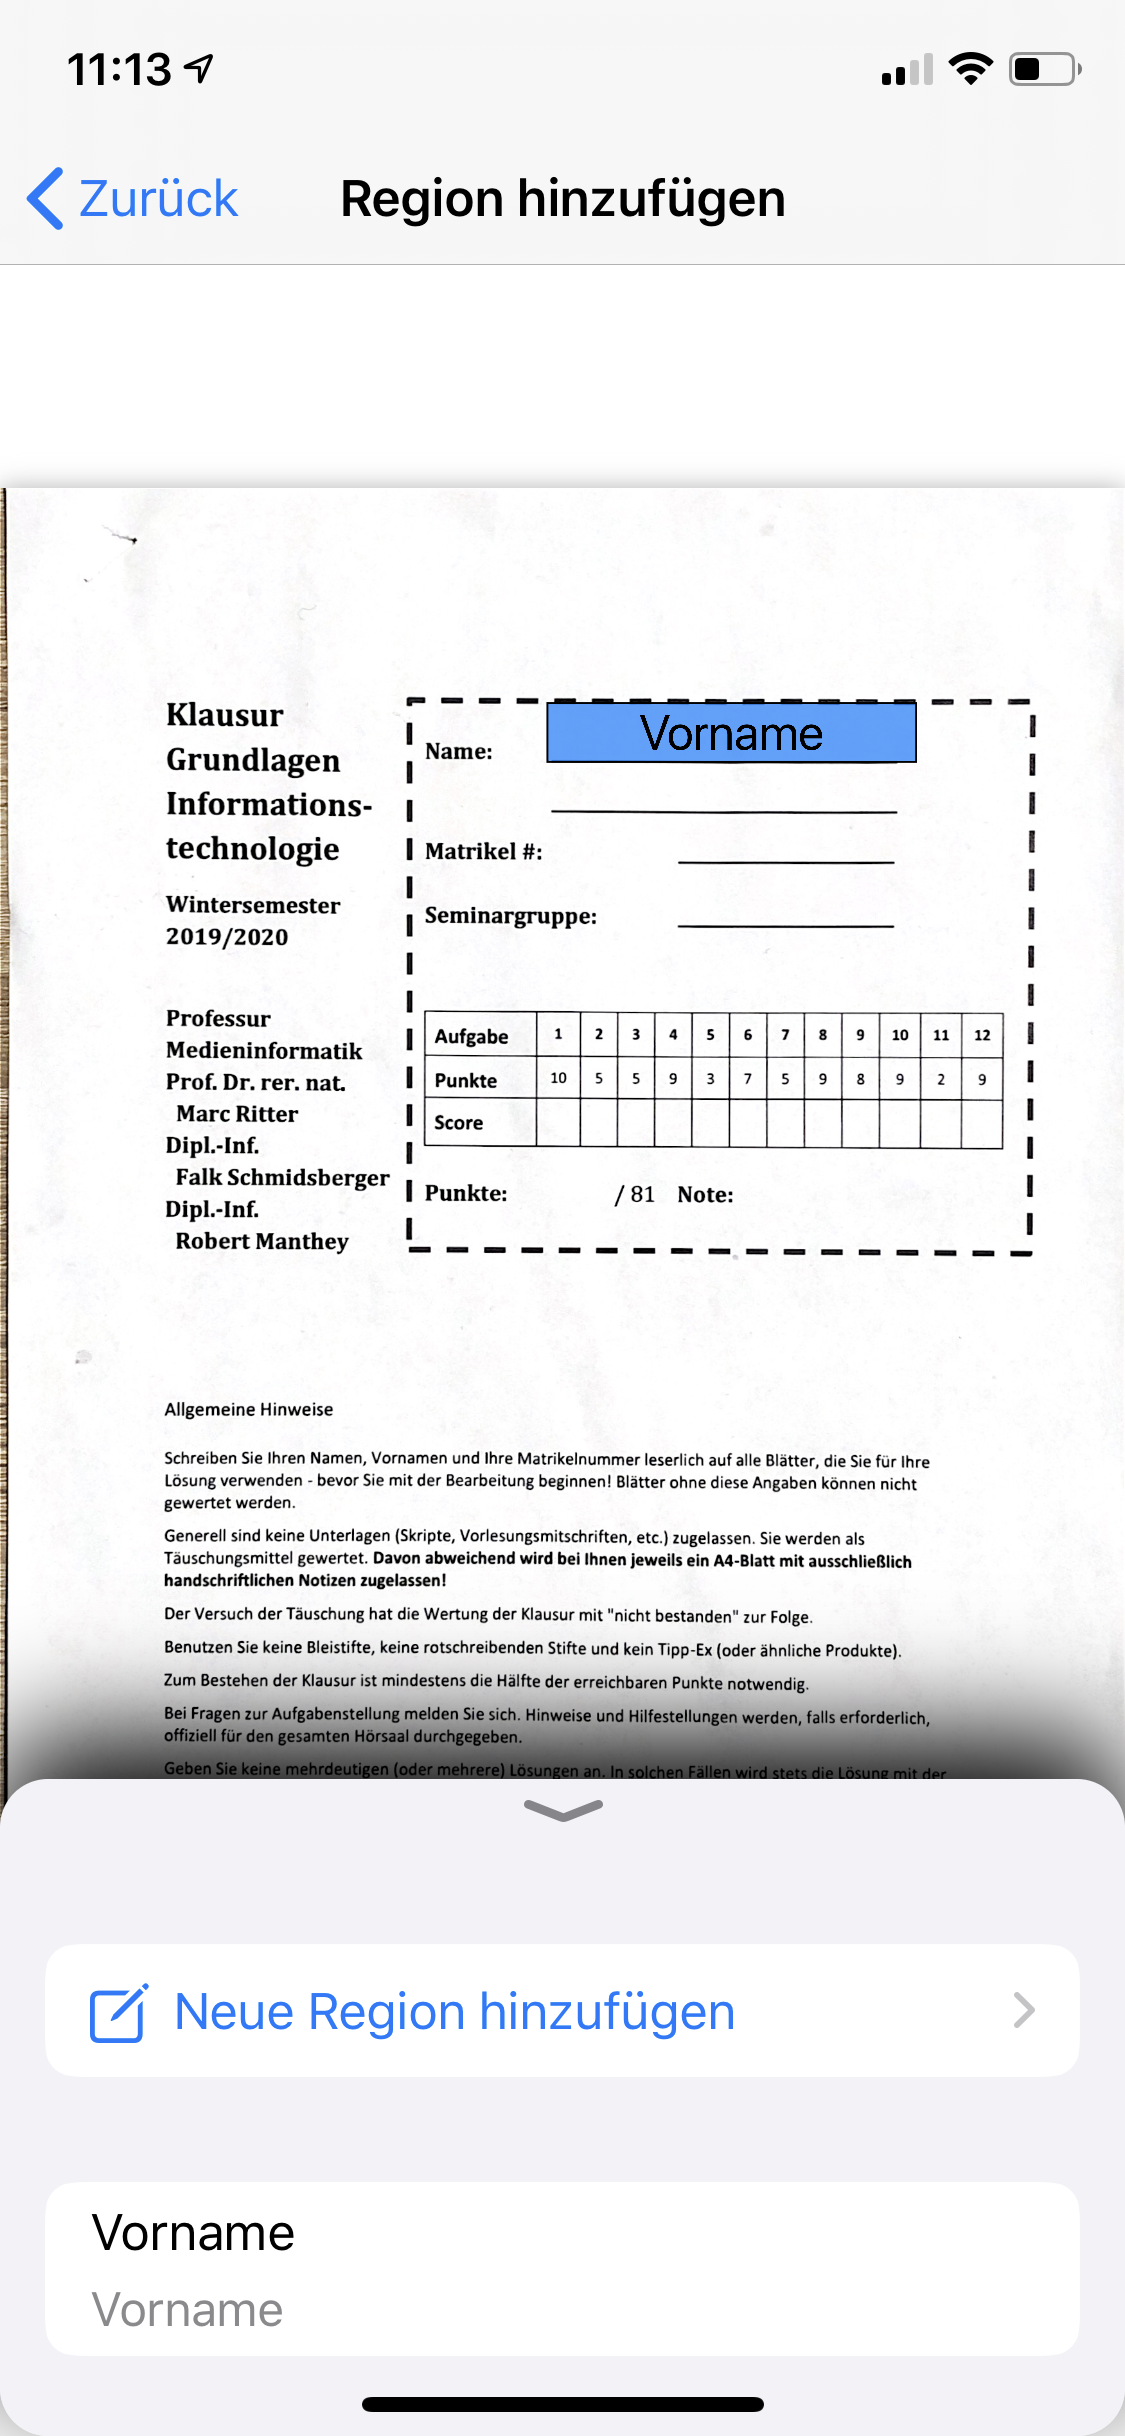
\includegraphics[width=0.96\textwidth]{img/V8}}
        	\caption{Seiten-Vorschau mit der ersten Region}
        	\label{fig:v8}
    	\end{subfigure}
    	\begin{subfigure}[t]{0.3\textwidth}
       		\frame{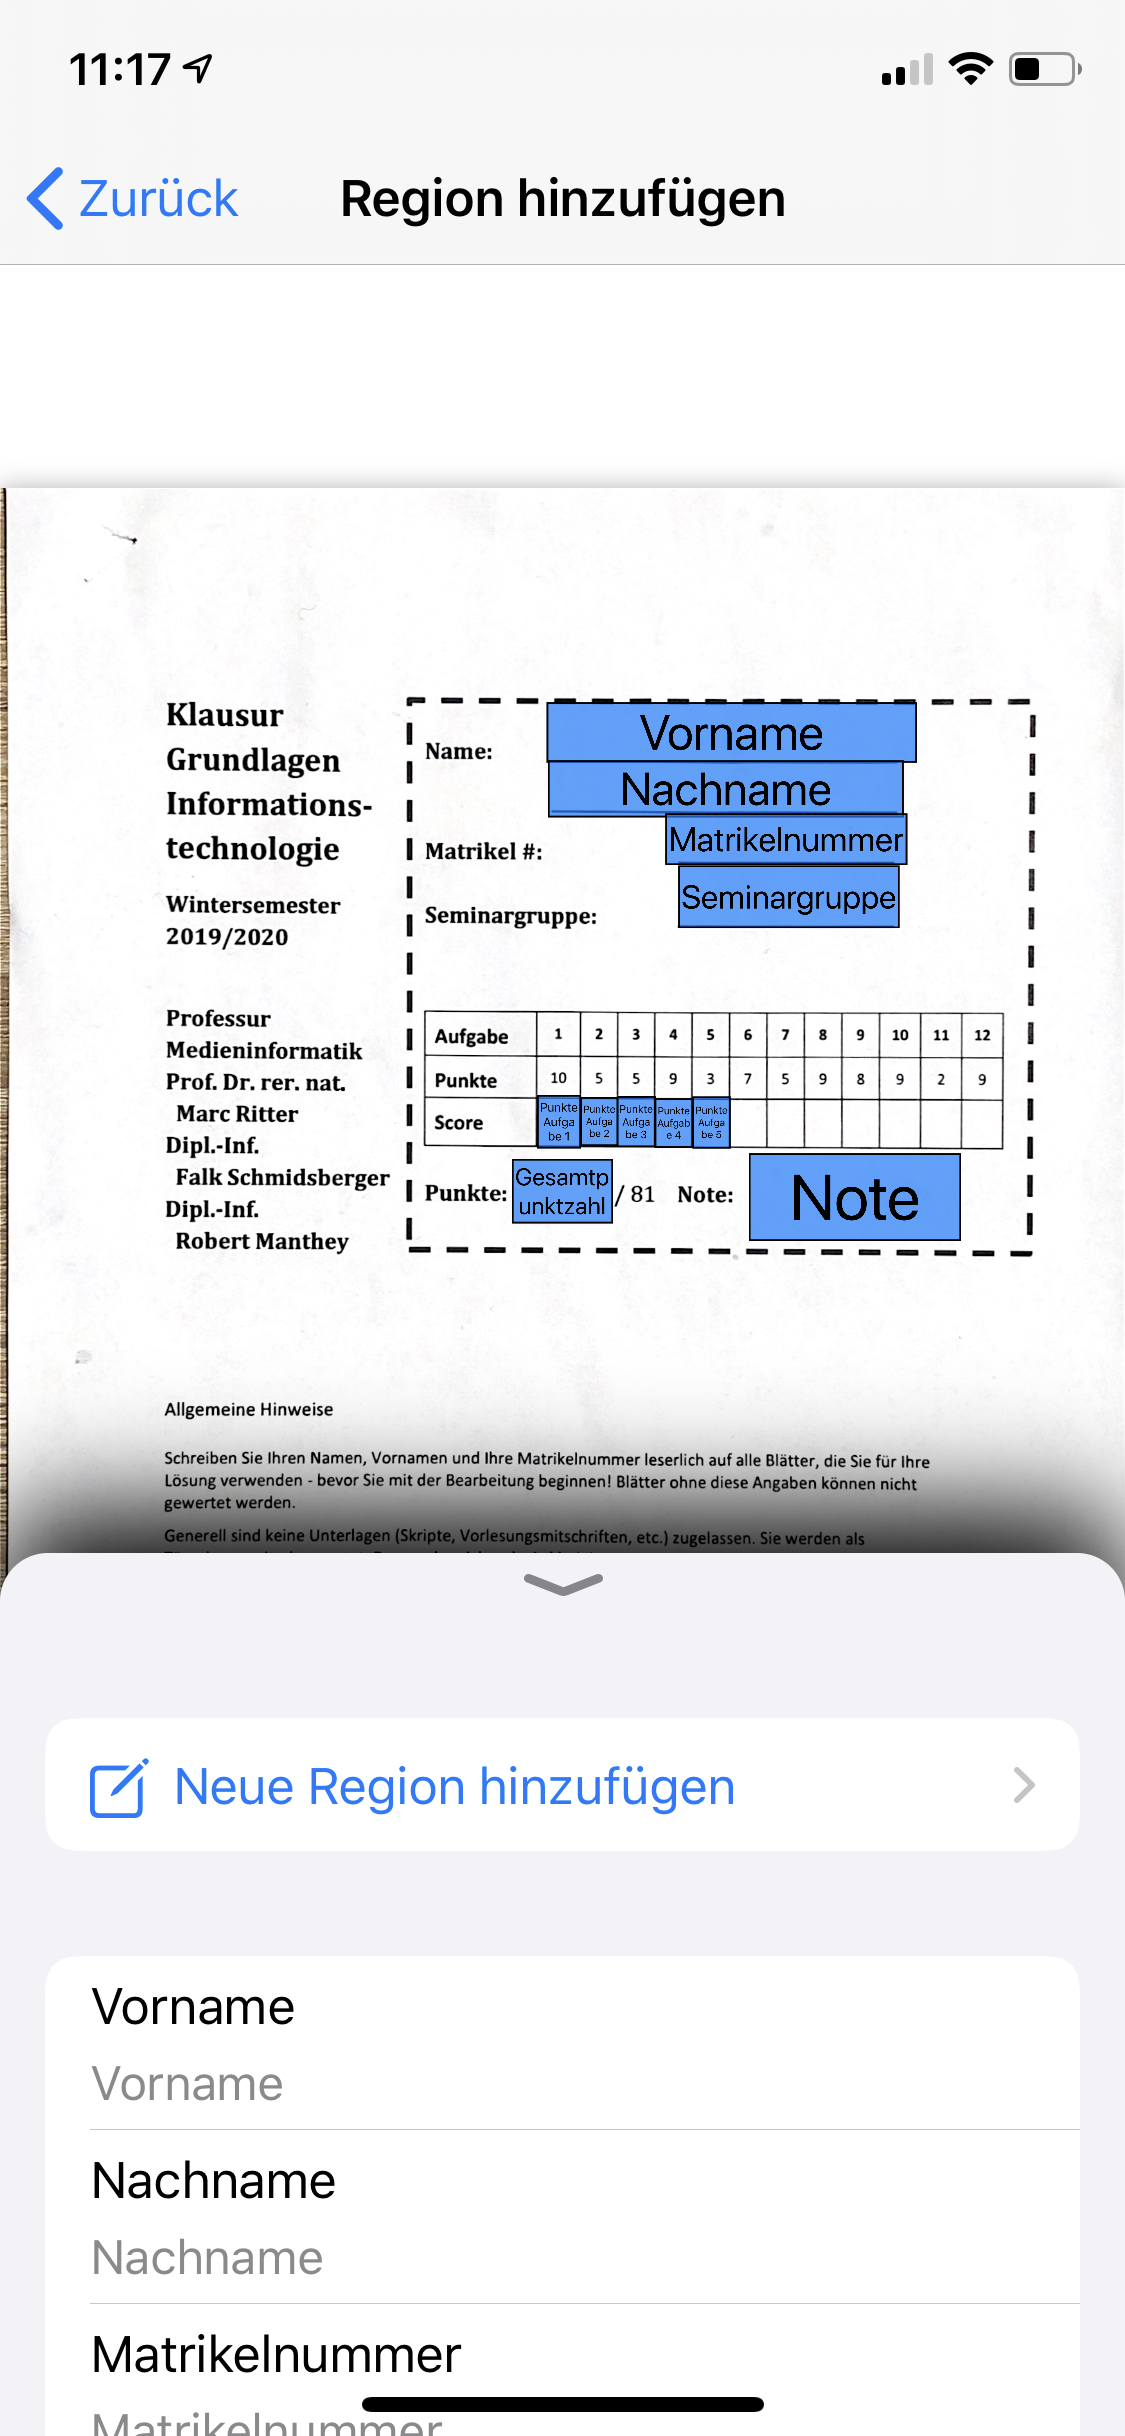
\includegraphics[width=0.96\textwidth]{img/V9}}
        	\caption{Seiten-Vorschau mit allen Regionen}
        	\label{fig:v9}
    	\end{subfigure}
    	\begin{subfigure}[t]{0.3\textwidth}
       		\frame{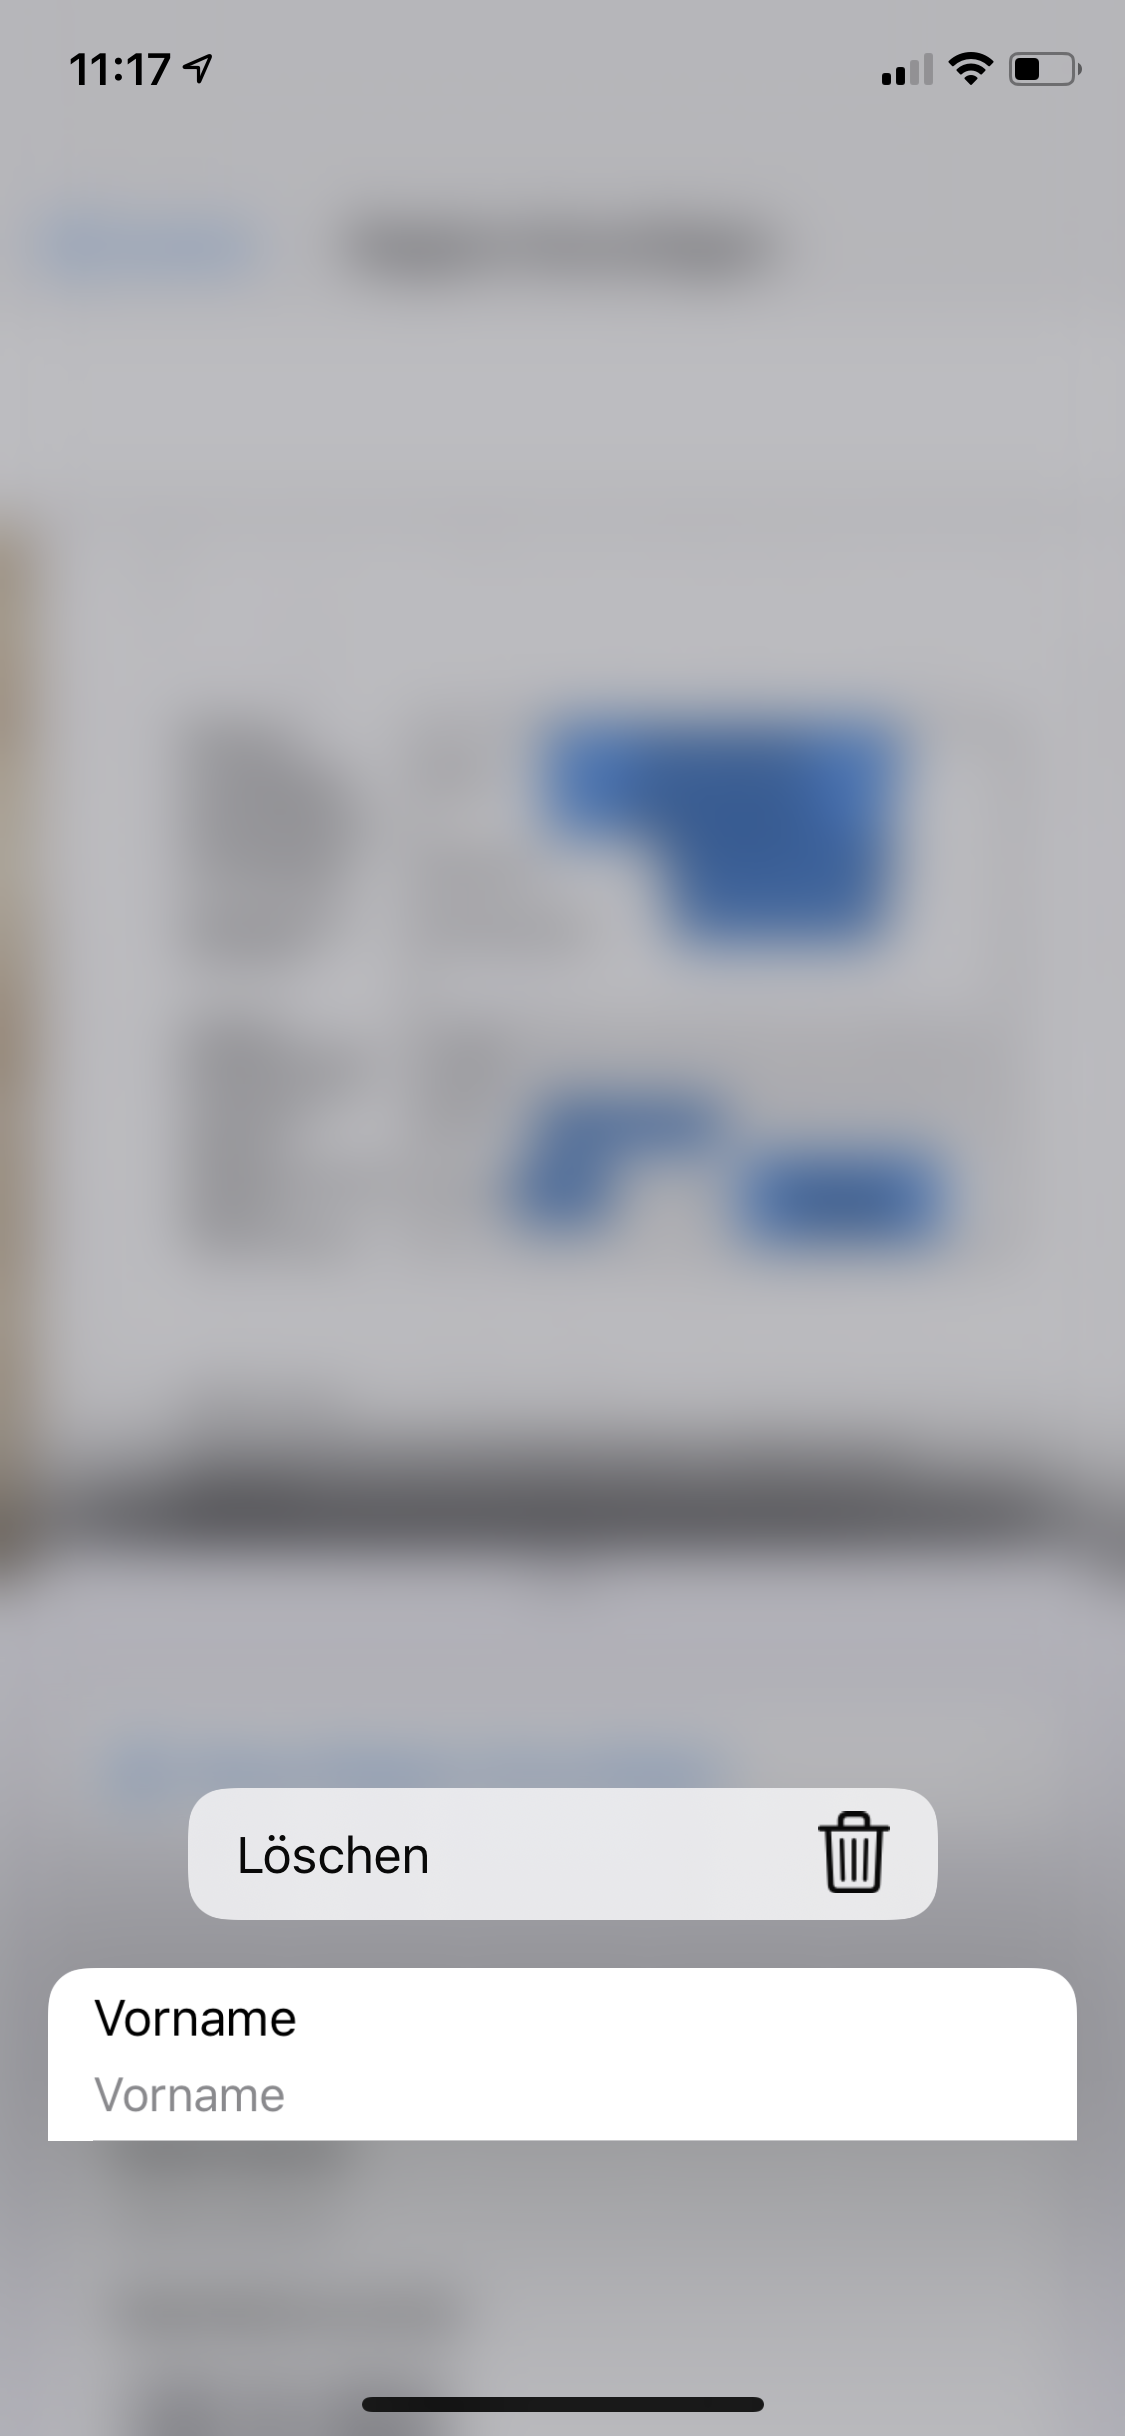
\includegraphics[width=0.96\textwidth]{img/V10}}
        	\caption{Löschen einer angelegten Region}
        	\label{fig:v10}
    	\end{subfigure}
    	\caption{Seiten-Vorschau-View}
		\label{fig:zusatz1}
	\end{figure}
	
	\begin{figure}[h]
		\centering
		\begin{subfigure}[t]{0.3\textwidth}
       		\frame{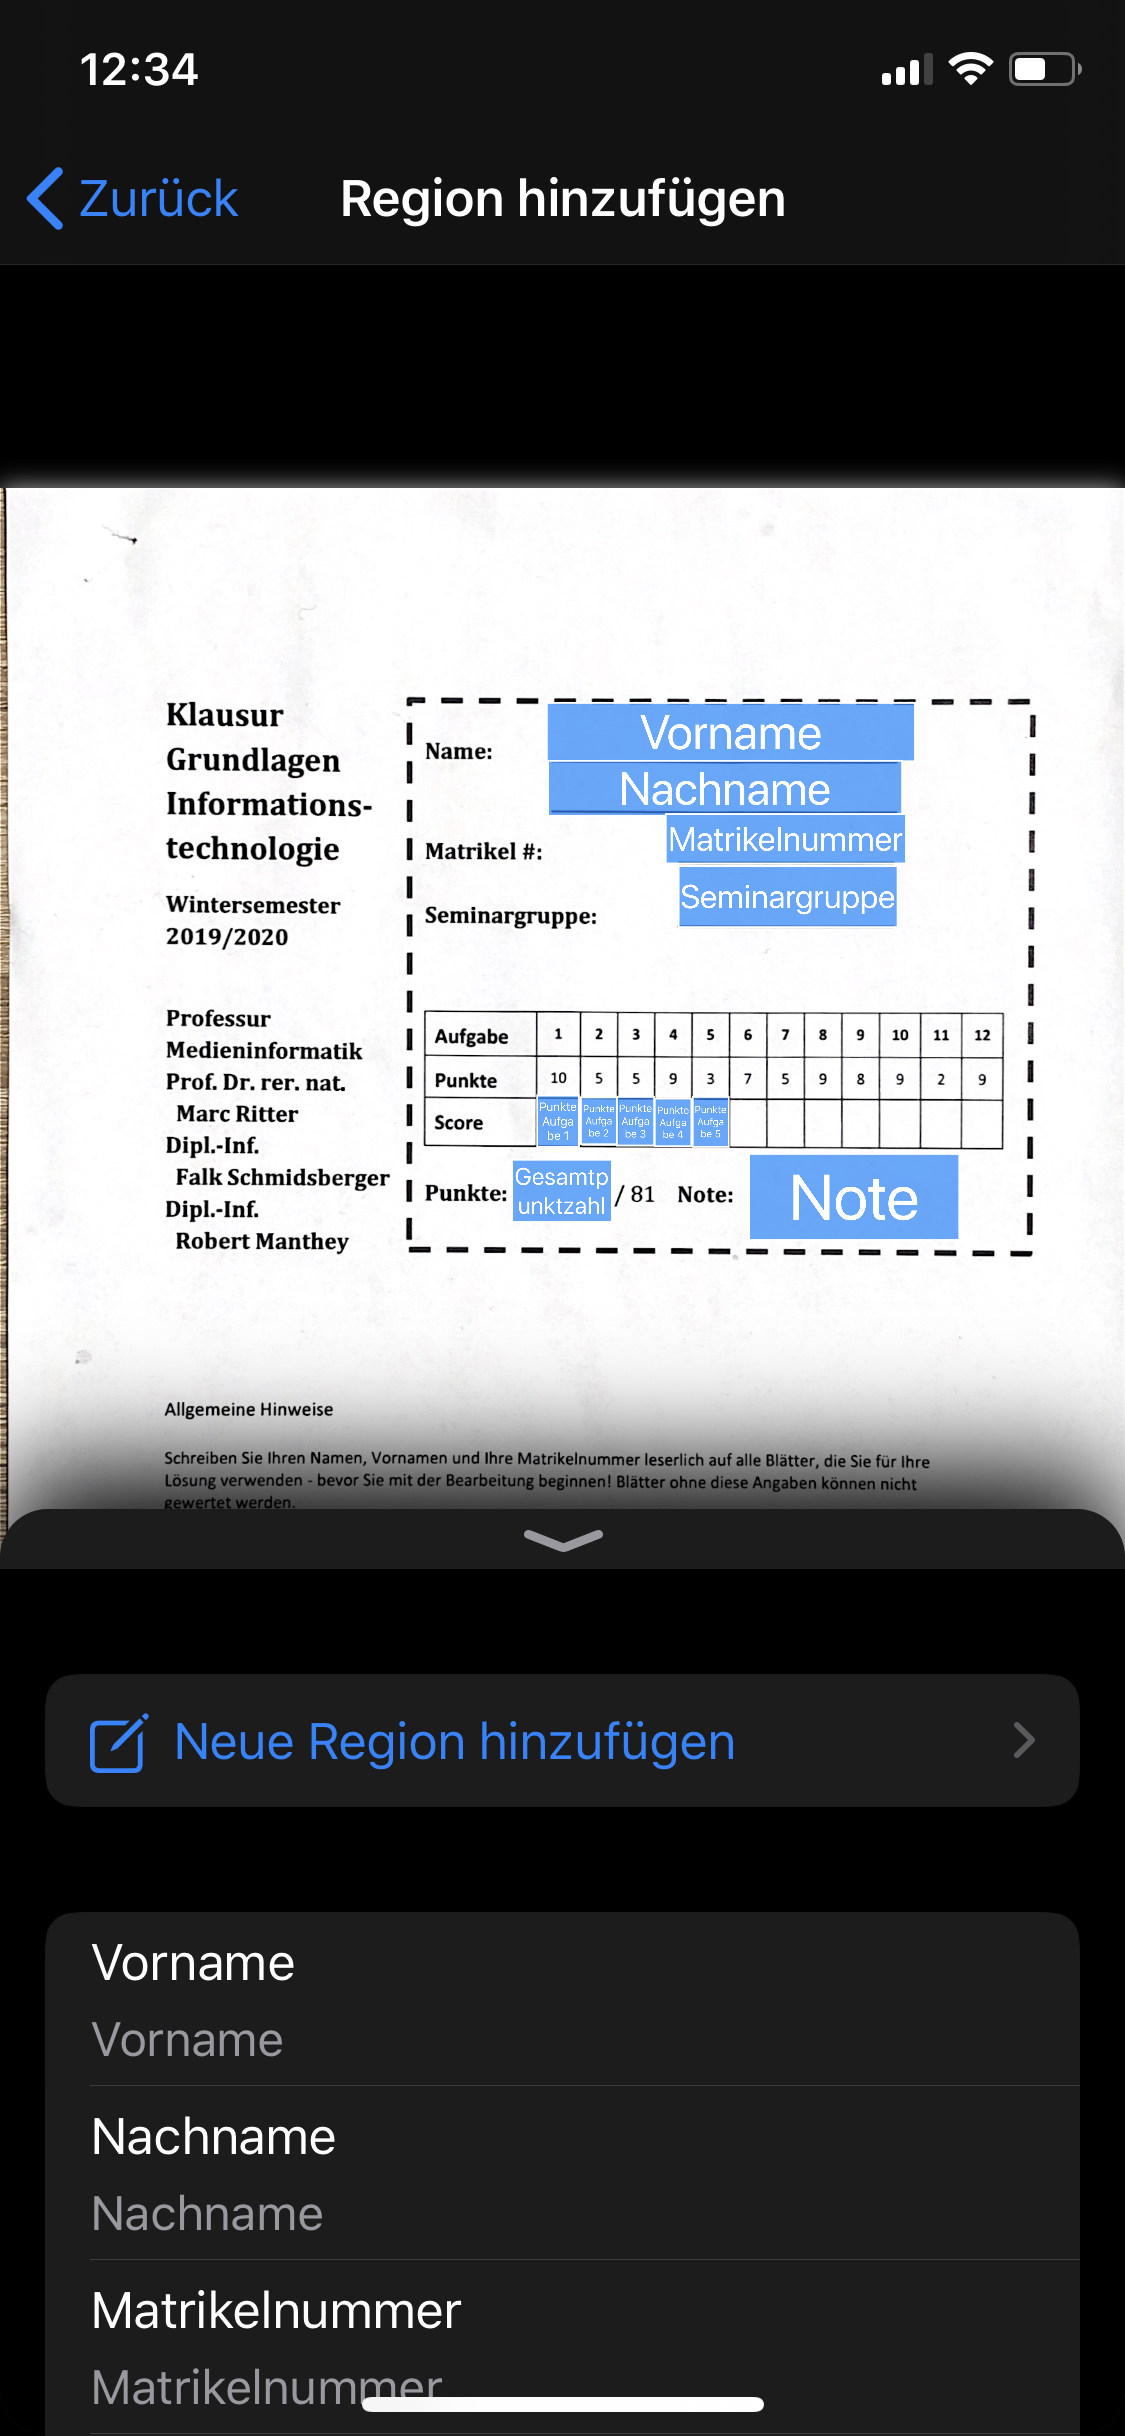
\includegraphics[width=0.96\textwidth]{img/z1}}
        	\caption{Seiten-Vorschau der 1. Seite mit allen Regionen im Dark-Mode}
        	\label{fig:l5}
    	\end{subfigure}
		\begin{subfigure}[t]{0.3\textwidth}
       		\frame{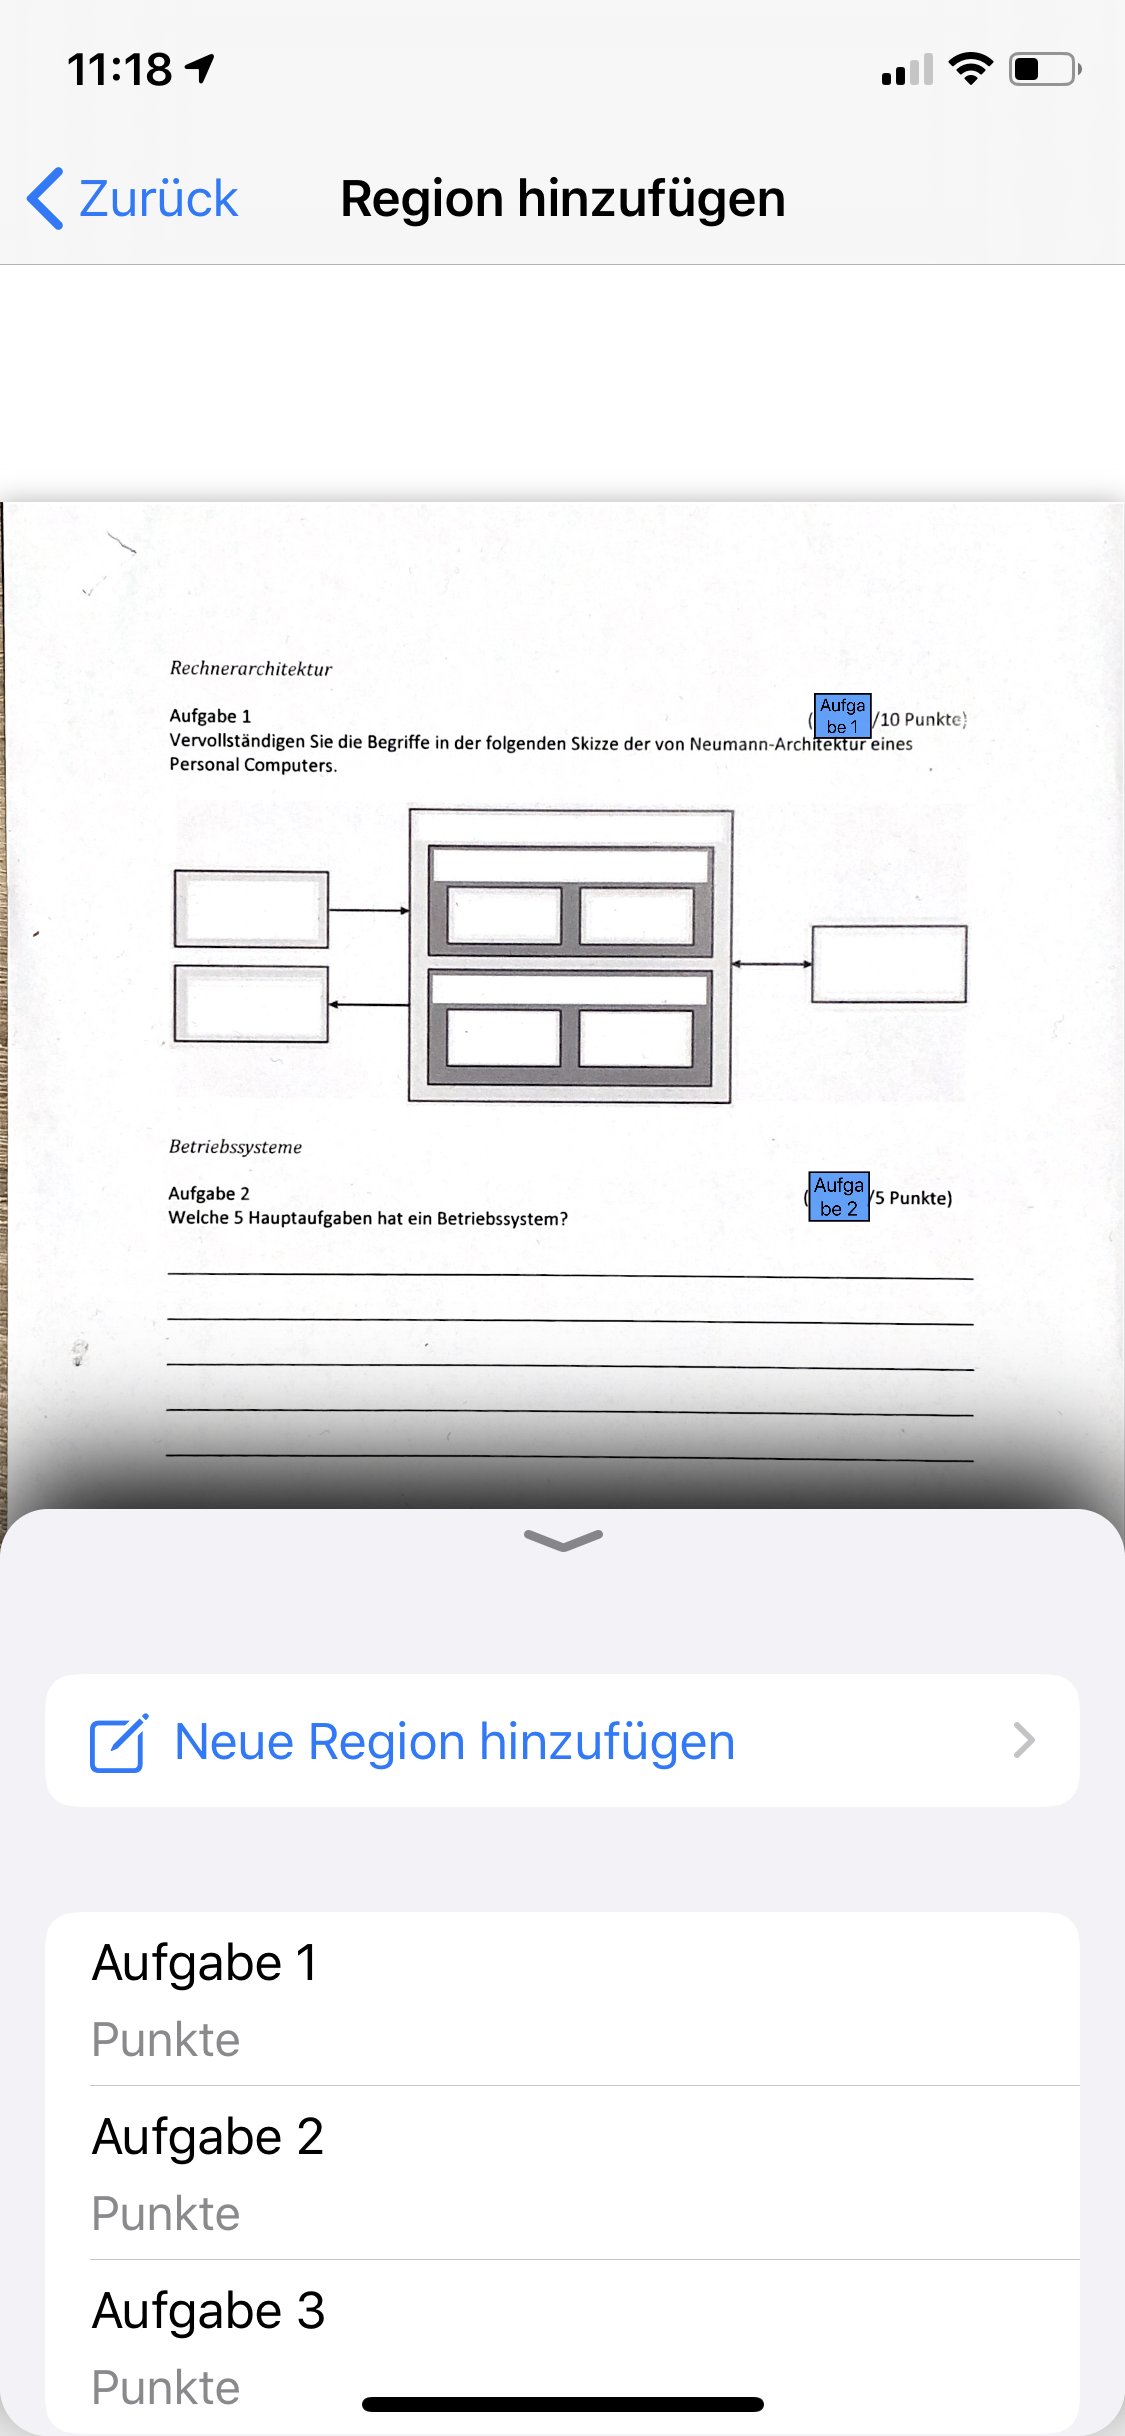
\includegraphics[width=0.96\textwidth]{img/V11}}
        	\caption{Seiten-Vorschau der 2. Seite mit allen Regionen}
        	\label{fig:v11}
    	\end{subfigure}
    	\begin{subfigure}[t]{0.3\textwidth}
       		\frame{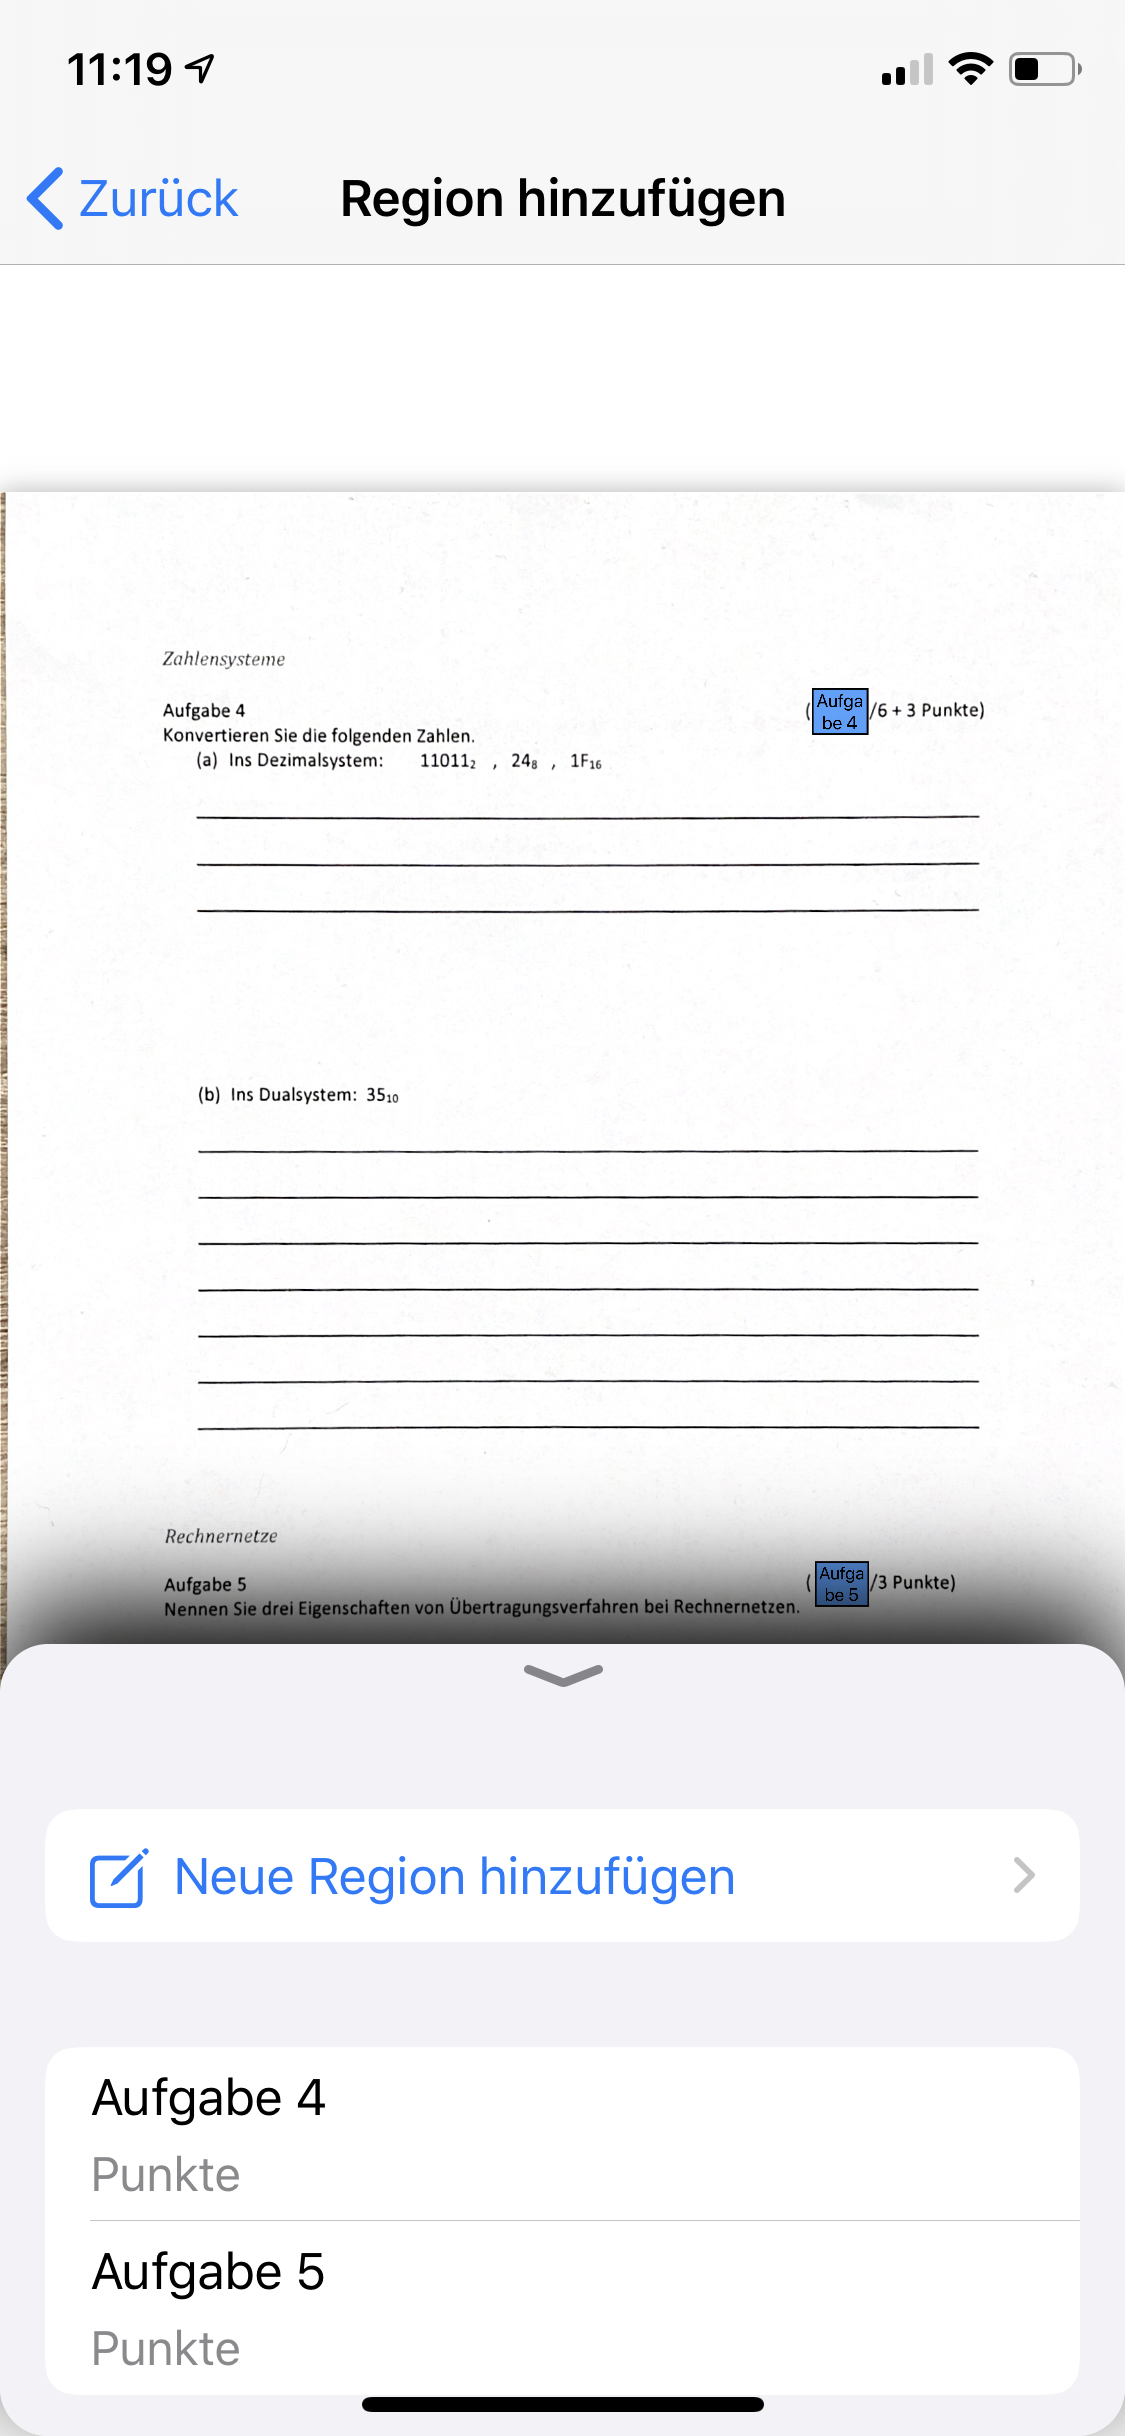
\includegraphics[width=0.96\textwidth]{img/V12}}
        	\caption{Seiten-Vorschau der 3. Seite mit allen Regionen}
        	\label{fig:v12}
    	\end{subfigure}
    	
    	\caption{Seiten-Vorschau im Light- und Dark-Mode}
		\label{fig:zusatz3}
	\end{figure}
	
	\begin{figure}[h]
		\centering
		\begin{subfigure}[t]{0.3\textwidth}
       		\frame{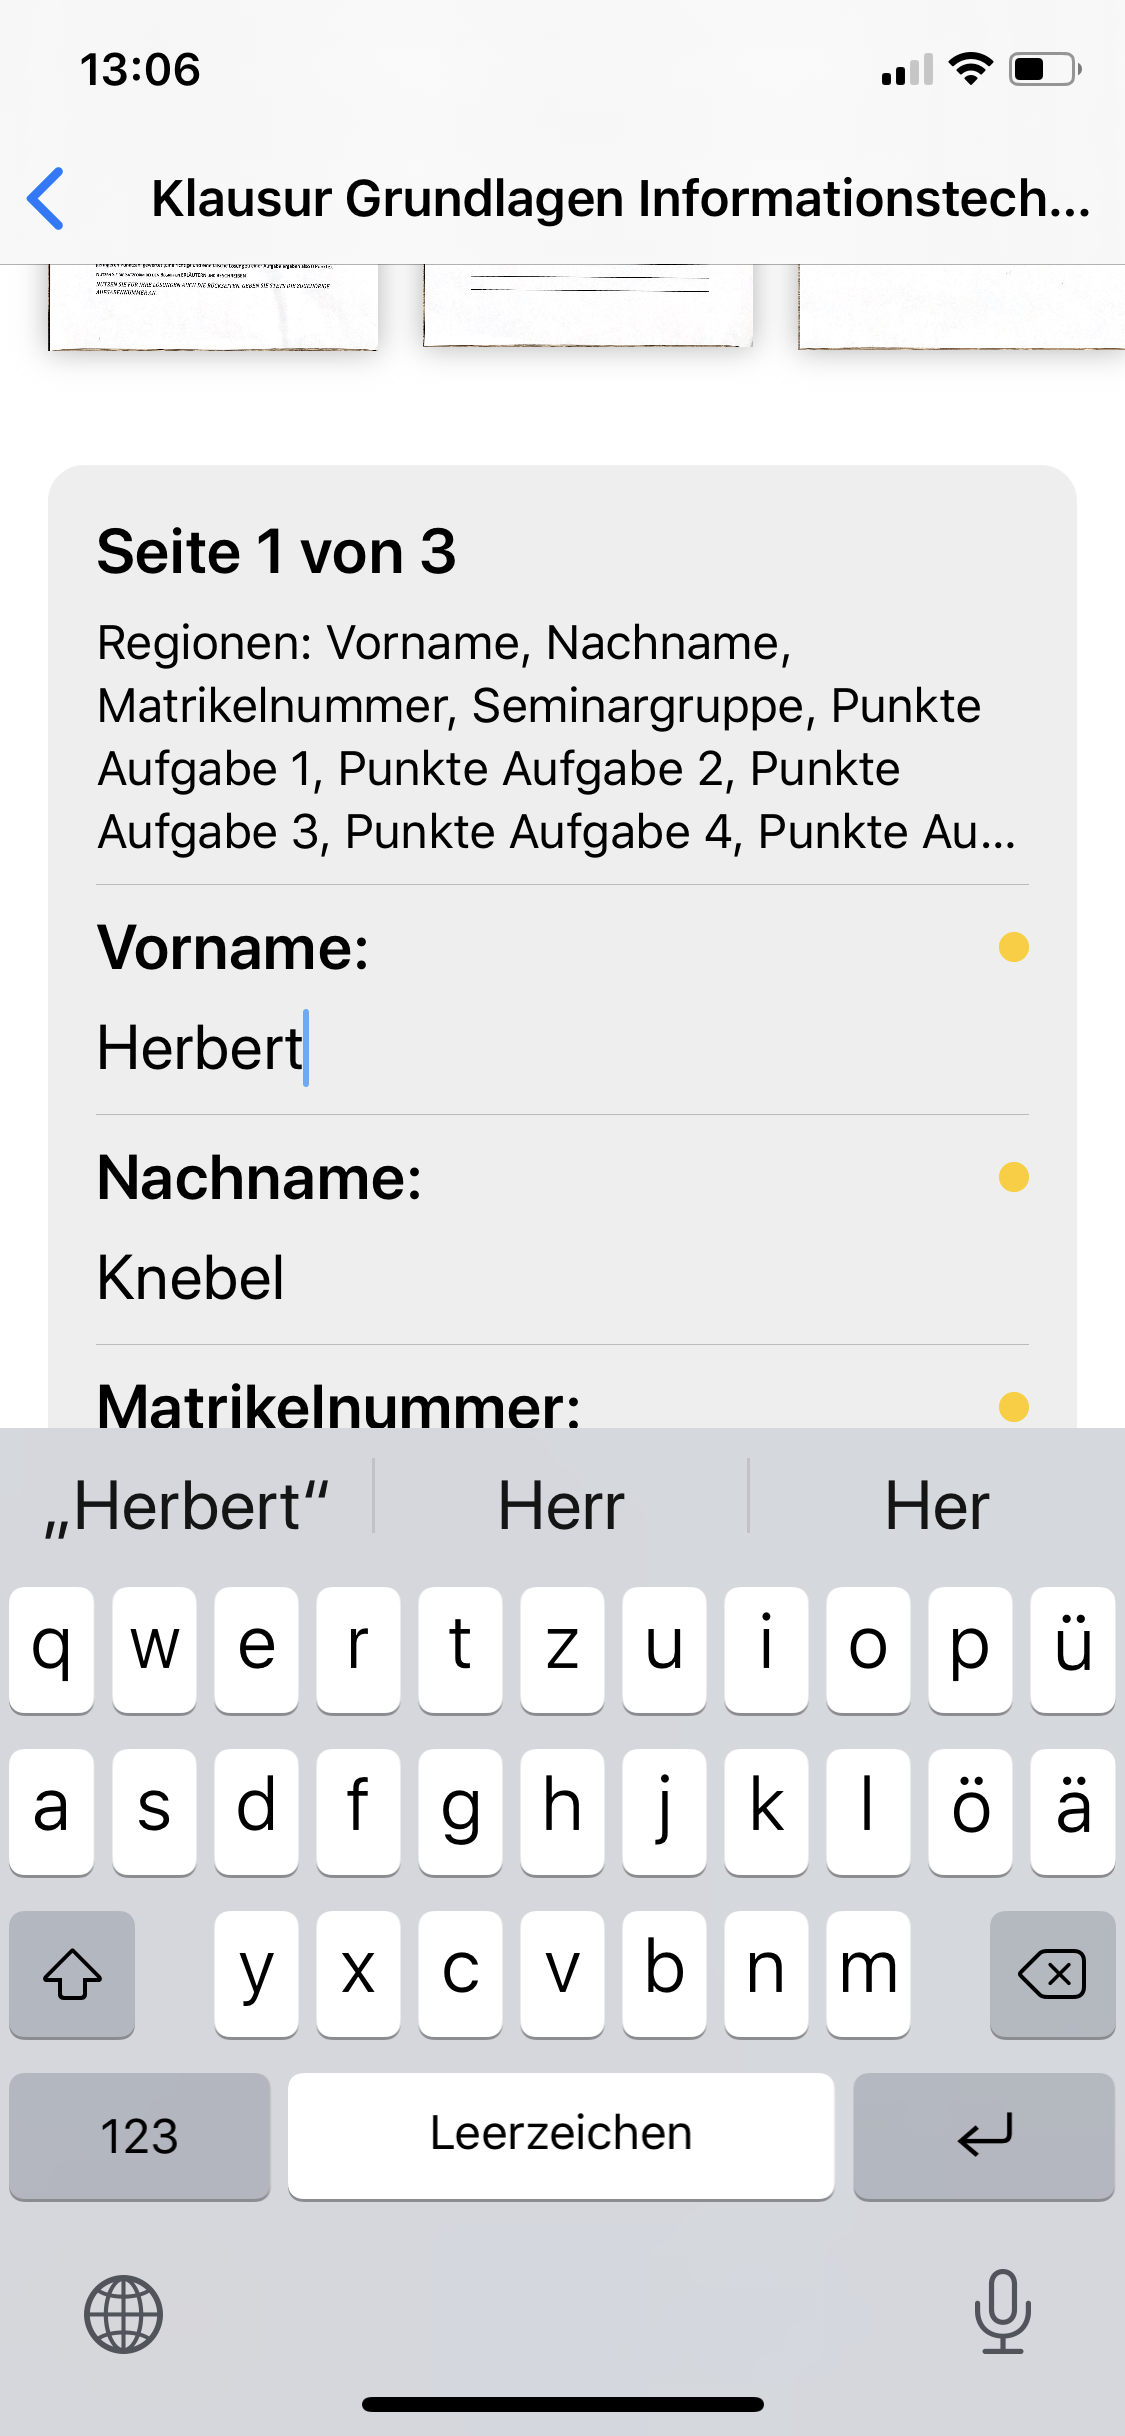
\includegraphics[width=0.96\textwidth]{img/z4}}
        	\caption{Ergebnis bearbeiten mit der größten einstellbaren Textgröße}
        	\label{fig:z4}
    	\end{subfigure}
		\begin{subfigure}[t]{0.3\textwidth}
       		\frame{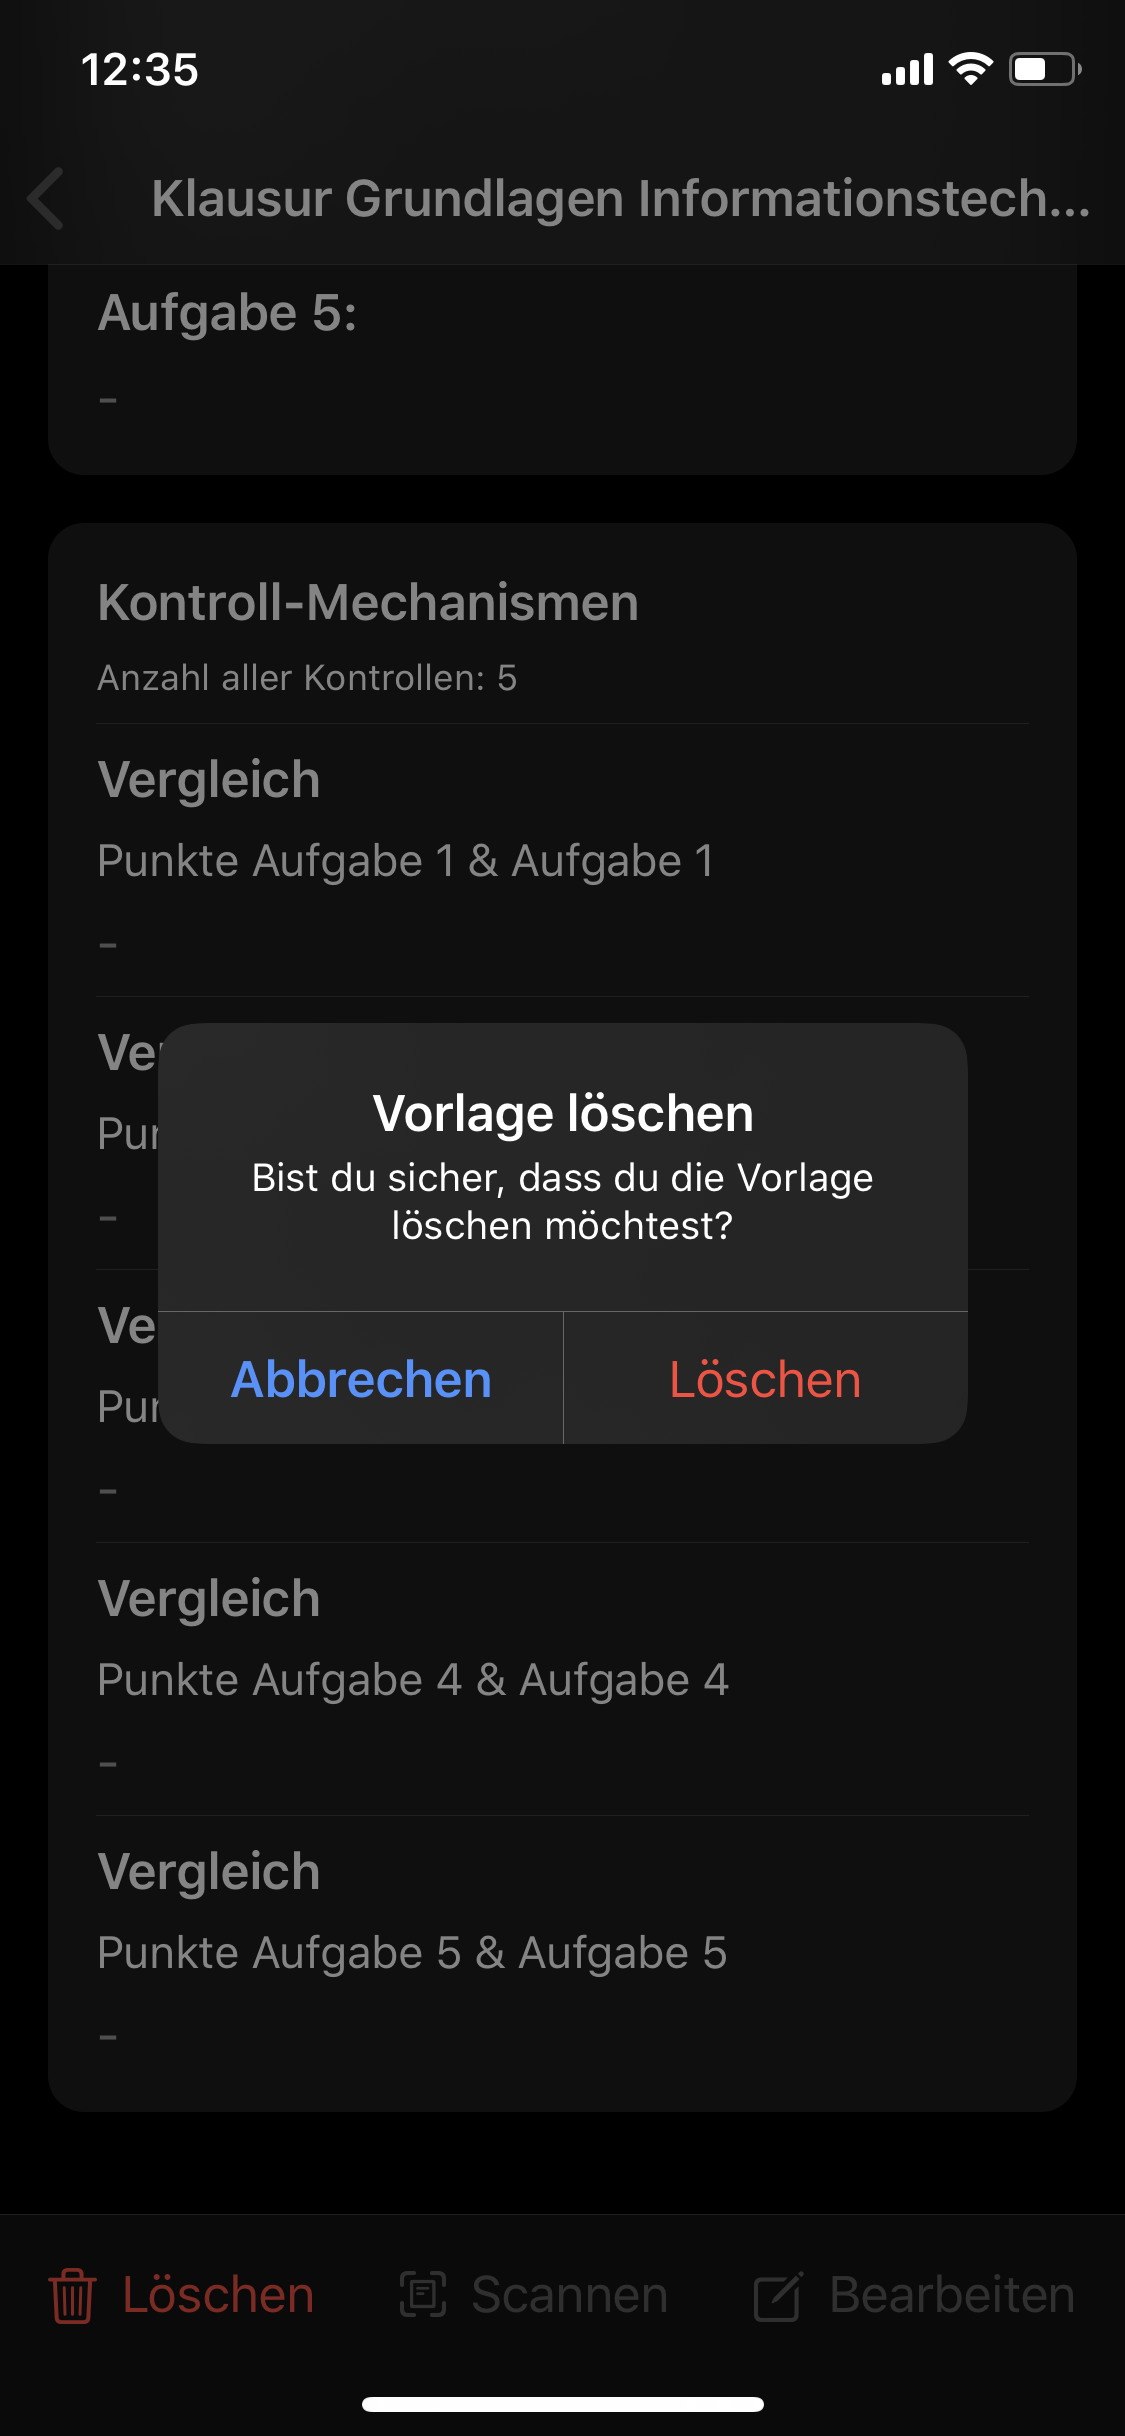
\includegraphics[width=0.96\textwidth]{img/z2}}
        	\caption{Löschen einer Vorlage im Dark-Mode}
        	\label{fig:z2}
    	\end{subfigure}
    	\begin{subfigure}[t]{0.3\textwidth}
       		\frame{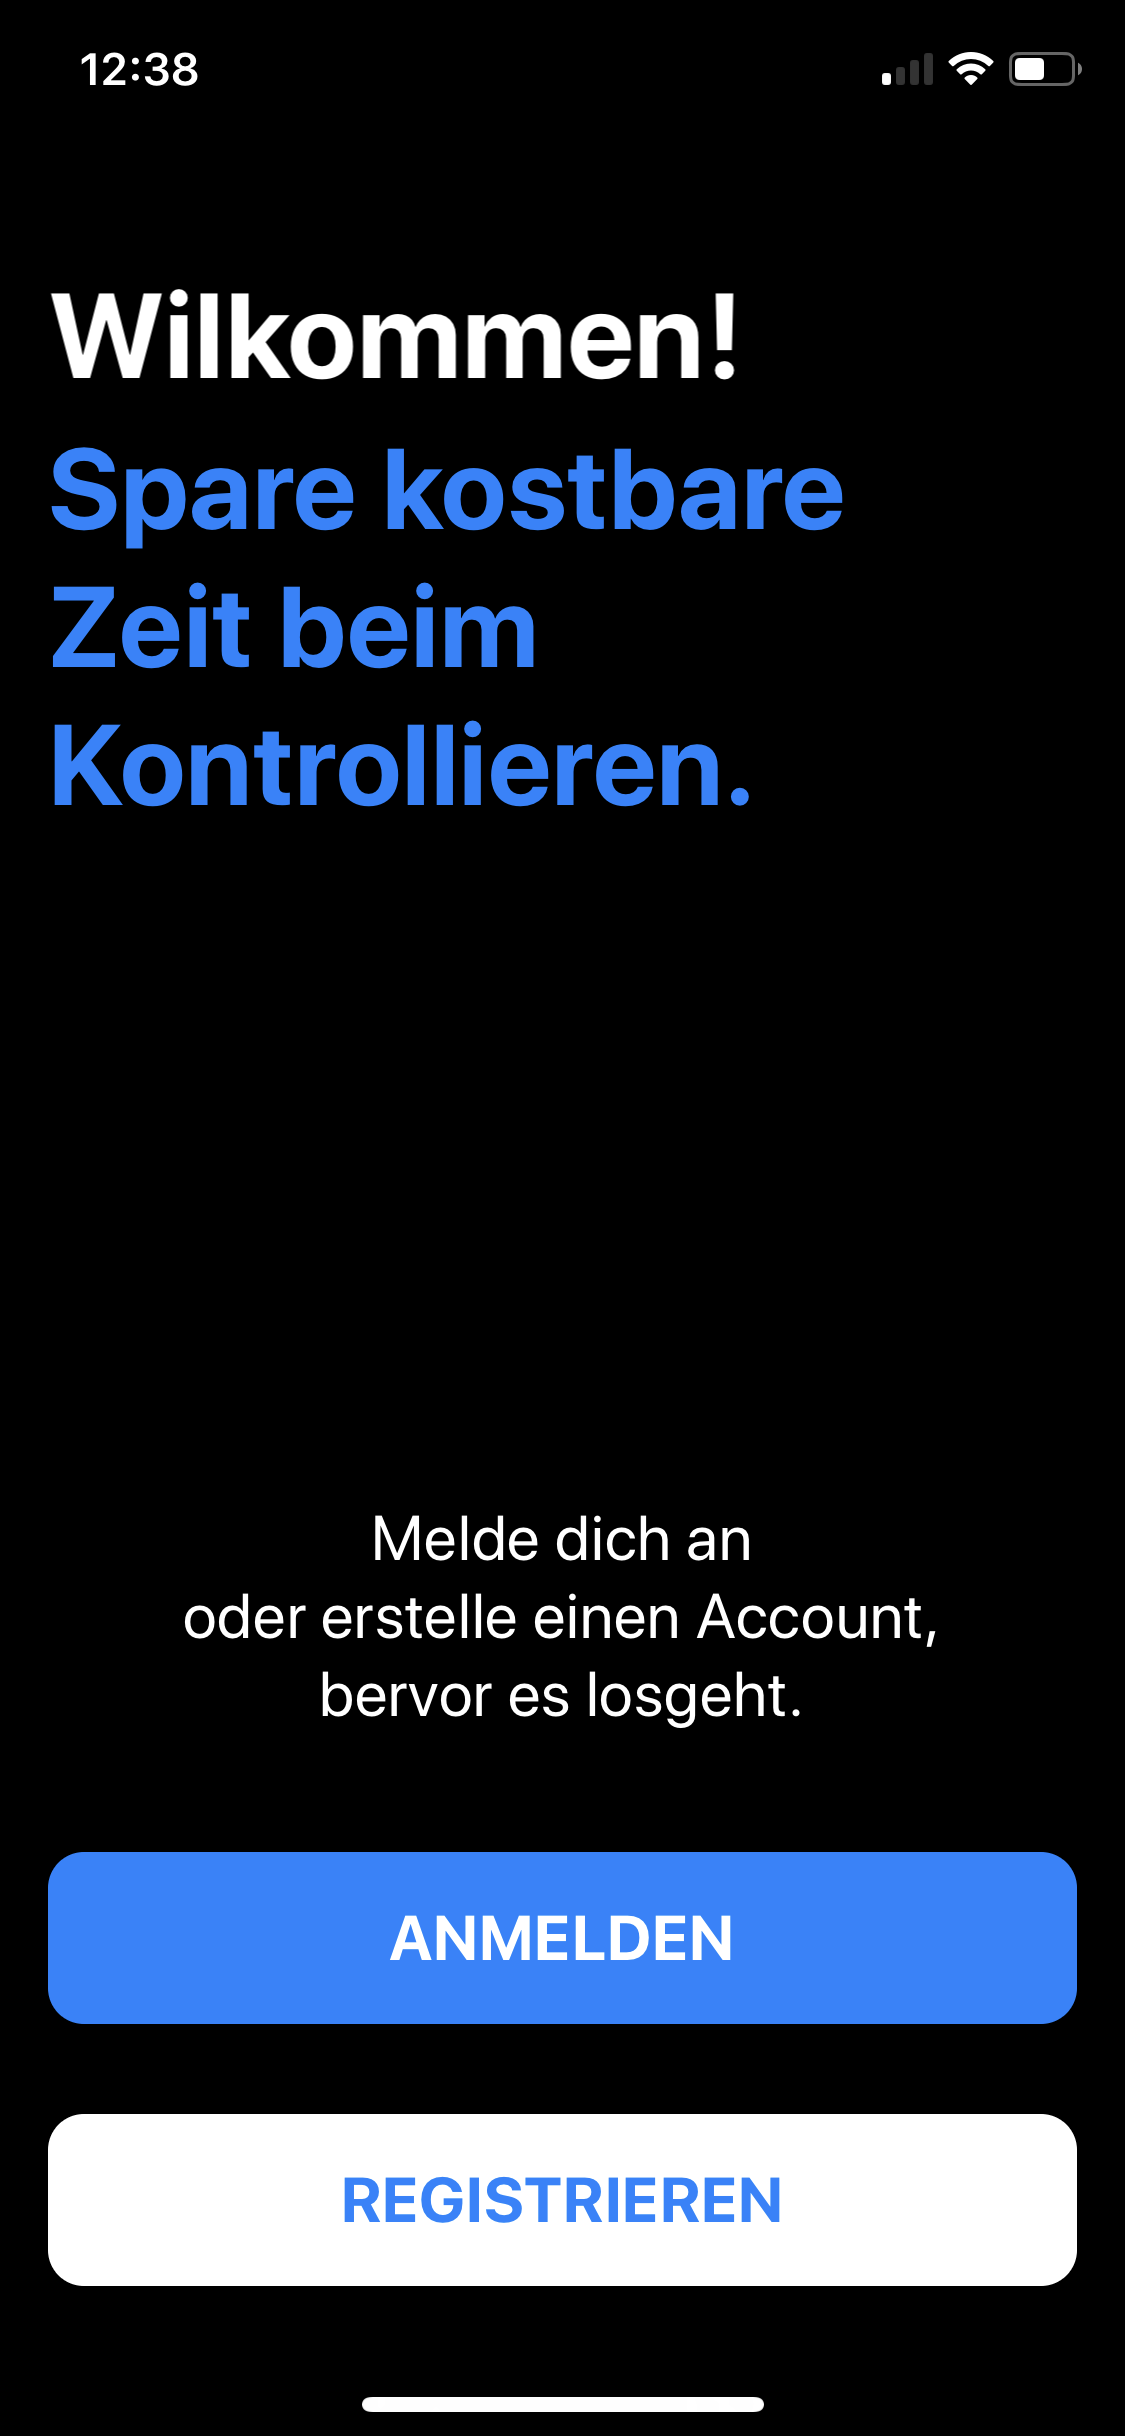
\includegraphics[width=0.96\textwidth]{img/z3}}
        	\caption{Willkommens-View mit der größten einstellbaren Textgröße}
        	\label{fig:z3}
    	\end{subfigure}
    	\caption{Barrierefreiheit und Dark-Mode Beispiele}
		\label{fig:zusatz4}
	\end{figure}
	
	
\chapter{Installation der iOS App}\label{ch:installation}
	Im folgenden Kapitel ist beschrieben, wie die App auf einem iPhone oder iPad zu installieren ist.
	
	\textbf{Vorraussetzungen:}
	\begin{itemize}
		\item macOS ab Version 10.15.4 
		\item Xcode ab Version 11.4.1 
		\item iPhone ab Version iOS 13.0 und/oder iPad ab Version iPadOS 13.4 
		\item Internetzugang
	\end{itemize}
	
	\textbf{Installation:}
	Stelle sicher, dass Xcode installiert und das iPhone/iPad mit dem Mac über ein USB-Kabel verbunden ist.
	\begin{enumerate}
		\item Lade das Projekt herunter. (.zip anschließend entpacken)
		\item Öffne die Datei \textit{DocumentenScanner.xcodeproj} mit Xcode.
		\item Klicke in der Ordnerübersicht bzw. im Navigator ganz oben auf das Xcode-Projekt \textit{DocumentenScanner}.
		\item Wähle im Editor-Fenster unter \textit{Targets} das Projekt \textit{DocumentenScanner} aus. (Entweder links oben als Dropdown-Menü oder im geöffneten Menü links innerhalb des Editor-Fensters.)
		\item Wähle den Reiter \textit{Signing \& Capabilities} aus. Es erscheint im Editor-Fenster ein Unterpunkt \textit{Signing}.
		\item Wähle ein passendes Team aus oder lege eins an.
		\item Ändere den Bundle Identifier passend zum ausgewählten Team. Z. B. \url{com.<Teamname>.DocumentenScanner}. Es taucht ein Button auf, mit dem die App signiert werden muss. Falls kein Button erscheint, gehe zum nächsten Schritt und komme bei einer auftretenden Fehlermeldung bezüglich der Signierung hierher zurück. (Die Internetverbindung wird benötigt.)
		\item Wähle nun einen Simulator oder das angeschlossene Gerät in der Toolbar aus den \textit{Active Devices} aus.
		\item Drücke anschließend den Start bzw. Run Button der \textit{Build Controls} oder die Tastenkombination \textbf{cmd + R}.
		\item Folge den Anweisungen von Xcode und auf dem iPhone oder iPad. Beim Verwenden eines Simulators tauchen keine weiteren Anweisungen auf. Die App startet automatisch. 
	\end{enumerate}
	

\chapter{Tätigkeitsbericht}
	\textbf{24.02. - 01.03.}
	Zunächst habe ich mich mit der Problemstellung auseinander gesetzt, Ideen gesammelt, Problemanalyse betrieben und einen kleinen Prototypen entwickelt. Dazu erstellte ich eine minimale Projektplanung, arbeitete mich in die Frameworks \textit{Vision} und \textit{VisionKit} ein und setzte eine Versionsverwaltung auf. Zusätzlich suchte ich nach einer passenden App-Architektur, die für das deklarative GUI-Framework SwiftUI sowie für asynchrone Aufgaben, wie z. B. API-Aufrufe geeignet ist. Dabei stieß ich auf \textit{Cleancode Architecture} und \textit{Redux}.
	
	\textbf{02.03. - 08.03.} 
	In dieser Woche habe ich die Texterkennung auf den berechneten Regionen eines neuen Fotos implementiert, den Workflow sowie viele andere Kleinigkeiten in der App verbessert und alle Fehler der letzten Woche behoben, sodass ich neue Dinge implementieren konnte. Zudem probierte ich CI sowie Lint für das Projekt aus. Da CI für eine iOS-App mit \textit{GitHub Actions} schwer aufzusetzen war und ab April kostenpflichtig wurde, verwarf ich meine Pläne. Des Weiteren pflegte ich das Projekt Management durch \textit{Issues} und \textit{Project Boards} in GitHub. Anschließend programmierte ich den App-Workflow so um, dass nun mehr als eine Seite aufgenommen und analysiert werden konnte. \\ 			
	Abgesehen von neuen Quellcode begann ich mit dem Schreiben des Praktikumsberichts und arbeitete mich dazu in \LaTeX \xspace und die Bachelorarbeit-Vorlage für \LaTeX \xspace der Hochschule Mittweida ein.
	
	\textbf{09.03. - 15.03.} 
	Zu Beginn der dritten Woche schaute ich mir Möglichkeiten für serverseitiges OCR an. Dabei sammelte ich Informationen zu dem Framework Vapor und Swift unter Linux. Da die Frameworks \textit{Vision} und \textit{CoreML} von \textit{Apple} unter Linux nicht funktionierten, stellte sich IronOCR als beste Option herausstellte. Mithilfe der in der App verwendeten Datentypen entwickelte ich ein Datenbankmodell und erstellte dazu noch eine JSON-Struktur, die später für die APIs verwendet werden könnte. Außerdem gab es ein Meeting, in dem Tobias Kallauke und ich unseren aktuellen Stand präsentierten, um weitere Schritte und Aufgaben zu planen. Bis zum Ende der Woche arbeitete ich fortlaufend an meinem Beleg und schrieb den Datenfluss in der App um. Nun ähnelte er sehr dem Redux-Model.
	
	\textbf{16.03. - 22.03.} 
	Anfangs schrieb ich meinen Praktikumsbericht weiter, bearbeitete alte Issues und fügte neue dem Project Board hinzu. Außerdem gepflegte ich die Dokumentation, um anschließend Kontrollmechanismen hinzuzufügen. Dabei entstanden neue Views. Der Redux-Store musste dadurch angepasst werden. Es kam eine Erweiterung für die Texterkennung hinzu, so dass man durch die Auswahl eines Datentyps, das Resultat der Erkennung verbessern konnte. Des Weiteren habe ich bis zum Ende der Woche den Kontroll-Typ \textit{Vergleich} vollständig implementiert und die App auf Fehler und Abstürze kontrolliert sowie den Beleg um einige Kapitel erweitert.
	
	\textbf{23.03. - 29.03.} 
	Ich begann den Workflow und die Navigation in der App zu verbessern und vereinfachen. Dabei beseitigte ich einigen Quellcode des Prototyps, erweiterte die Dokumentation und behob einige Fehler. Anschließend überarbeitete ich einige Views, sodass sie übersichtlicher und einfacher zu benutzen sind. Nach dem iOS 13.4 Update Mitte der Woche funktionierte ein Teil der App nicht, da sich das Verhalten von Views geändert hatte. Ich behob die Fehler, testete ausgiebig die App und fügte iPad Unterstützung hinzu. Des Weiteren entstand eine neue verbesserte permanente Scan-Vorlgae und ich schrieb einen großen Teil des Berichts.
	
	\textbf{30.03. - 05.04.} 
	Das Backend für die App war soweit, dass ich es aufsetzten und die API-Schnittstellen implementieren konnte. Dazu erstellte ich Views für Registrieren und Anmelden, die mithilfe von regulären Ausdrücken, die Eingaben überprüfen. Außerdem entwickelte ich für die anfallenden asynchronen Aufgaben einen Schicht im App-Store. Dabei las ich mich in das Framework Combine ein und überlegte mir einen geeigneten Aufbau. Da der Ansatz von Combine sehr neu für mich war, dauerte es zwei Tage, bis ein erster API-Service mit Fehler-Handling funktionierte. Zum Ende der Woche waren alle der Create-Schnittstellen implementiert, getestet und dokumentiert. Nebenbei erstellte ein paar Issues für das Backend und sprach mich mit Tobias über OCR auf dem Server ab.
	
	\textbf{06.04. - 12.04.}
	Diese Woche startete mit dem Umschreiben der Kontroll-Mechanismen und deren Analyse. Anschließend integrierte ich die Neuerungen vom Backend und erstellte die API für den Upload von Bildern. Danach fügte ich die APIs zusammen, um Vorlagen vollständig auf dem Server zu speichern und ab zu rufen. Dazu schrieb ich eine eigene JSON-Decoder-Funktion, um die App internen Datentypen zu unterstützen. Zusätzlich wurde die App etwas benutzerfreundlicher und ein Problem mit dem Start der iPad Version wurde behoben. Nach einem Meeting folgten noch weitere Absprachen mit Tobias und ich arbeitete weiter an dem Bericht.
	
	\textbf{14.04. - 19.04.}
	Ein kritisches Problem mit den Sessions der vorherigen Woche konnte in dieser endlich gelöst werden. Dazu konnte ich die Anwendung etwas optimieren und einen sehr großen Teil des Beleges fertig stellen. Dabei half auch die Beantwortung vieler Fragen während eines Meetings mit dem Betreuer. Allerdings entstanden Probleme mit der Datenbank, die die Funktionalität der App einschränkten.
	
	\textbf{20.04. - 26.04.}
	Ziel dieser Woche war es, so viel wie möglich des Belegs zu schreiben. Dafür fertigte ich einige Schemata und Bilder an. Zusätzlich konnte ich einige Fehler der App analysieren und beheben, sodass die Performance verbessert und Server-Aufrufe eingespart wurden. Außerdem kam die Online-Texterkennung über den Server hinzu sowie die zweite Korrektur in der Texterkennung mit Vision. Jedoch konnte die Online-Texterkennung auf Grund von Server-Problemen nicht getestet werden. Auch in dieser Woche konnten einige Fragen zum Aufbau des Berichts in einem Meeting geklärt werden. 
	
	\textbf{27.04. - 03.05.}
	Im Mittelpunkt der Woche stand der Bericht, an dem ich täglich arbeitete. Ich erstellte einige Bilder für ihn und den Vortrag. Auch gab es diese Woche wieder ein Meeting.
	
	\textbf{04.05. - 10.05.}
	Auch diese Woche arbeitete ich hauptsächlich am Beleg und stellte ihn so weit fertig, dass nur noch wenige Dinge zu erledigen sind. Zudem gelang es Tobias die Fehler der online OCR-Engine Tesseract zu beseitigen. Dadurch konnte ich die letzten fehlenden Schritte für den Umgang mit den OCR-Schnittstellen implementieren und testen.
	
	\textbf{11.05. - 15.05.}


\bibliography{Beleg}
\bibliographystyle{iso690.bst}
\end{document}